\documentclass[twoside]{book}

% Packages required by doxygen
\usepackage{fixltx2e}
\usepackage{calc}
\usepackage{doxygen}
\usepackage[export]{adjustbox} % also loads graphicx
\usepackage{graphicx}
\usepackage[utf8]{inputenc}
\usepackage{makeidx}
\usepackage{multicol}
\usepackage{multirow}
\PassOptionsToPackage{warn}{textcomp}
\usepackage{textcomp}
\usepackage[nointegrals]{wasysym}
\usepackage[table]{xcolor}

% Font selection
\usepackage[T1]{fontenc}
\usepackage[scaled=.90]{helvet}
\usepackage{courier}
\usepackage{amssymb}
\usepackage{sectsty}
\renewcommand{\familydefault}{\sfdefault}
\allsectionsfont{%
  \fontseries{bc}\selectfont%
  \color{darkgray}%
}
\renewcommand{\DoxyLabelFont}{%
  \fontseries{bc}\selectfont%
  \color{darkgray}%
}
\newcommand{\+}{\discretionary{\mbox{\scriptsize$\hookleftarrow$}}{}{}}

% Page & text layout
\usepackage{geometry}
\geometry{%
  a4paper,%
  top=2.5cm,%
  bottom=2.5cm,%
  left=2.5cm,%
  right=2.5cm%
}
\tolerance=750
\hfuzz=15pt
\hbadness=750
\setlength{\emergencystretch}{15pt}
\setlength{\parindent}{0cm}
\setlength{\parskip}{3ex plus 2ex minus 2ex}
\makeatletter
\renewcommand{\paragraph}{%
  \@startsection{paragraph}{4}{0ex}{-1.0ex}{1.0ex}{%
    \normalfont\normalsize\bfseries\SS@parafont%
  }%
}
\renewcommand{\subparagraph}{%
  \@startsection{subparagraph}{5}{0ex}{-1.0ex}{1.0ex}{%
    \normalfont\normalsize\bfseries\SS@subparafont%
  }%
}
\makeatother

% Headers & footers
\usepackage{fancyhdr}
\pagestyle{fancyplain}
\fancyhead[LE]{\fancyplain{}{\bfseries\thepage}}
\fancyhead[CE]{\fancyplain{}{}}
\fancyhead[RE]{\fancyplain{}{\bfseries\leftmark}}
\fancyhead[LO]{\fancyplain{}{\bfseries\rightmark}}
\fancyhead[CO]{\fancyplain{}{}}
\fancyhead[RO]{\fancyplain{}{\bfseries\thepage}}
\fancyfoot[LE]{\fancyplain{}{}}
\fancyfoot[CE]{\fancyplain{}{}}
\fancyfoot[RE]{\fancyplain{}{\bfseries\scriptsize Generated by Doxygen }}
\fancyfoot[LO]{\fancyplain{}{\bfseries\scriptsize Generated by Doxygen }}
\fancyfoot[CO]{\fancyplain{}{}}
\fancyfoot[RO]{\fancyplain{}{}}
\renewcommand{\footrulewidth}{0.4pt}
\renewcommand{\chaptermark}[1]{%
  \markboth{#1}{}%
}
\renewcommand{\sectionmark}[1]{%
  \markright{\thesection\ #1}%
}

% Indices & bibliography
\usepackage{natbib}
\usepackage[titles]{tocloft}
\setcounter{tocdepth}{3}
\setcounter{secnumdepth}{5}
\makeindex

% Hyperlinks (required, but should be loaded last)
\usepackage{ifpdf}
\ifpdf
  \usepackage[pdftex,pagebackref=true]{hyperref}
\else
  \usepackage[ps2pdf,pagebackref=true]{hyperref}
\fi
\hypersetup{%
  colorlinks=true,%
  linkcolor=blue,%
  citecolor=blue,%
  unicode%
}

% Custom commands
\newcommand{\clearemptydoublepage}{%
  \newpage{\pagestyle{empty}\cleardoublepage}%
}

\usepackage{caption}
\captionsetup{labelsep=space,justification=centering,font={bf},singlelinecheck=off,skip=4pt,position=top}

%===== C O N T E N T S =====

\begin{document}

% Titlepage & ToC
\hypersetup{pageanchor=false,
             bookmarksnumbered=true,
             pdfencoding=unicode
            }
\pagenumbering{alph}
\begin{titlepage}
\vspace*{7cm}
\begin{center}%
{\Large Test\+Caser }\\
\vspace*{1cm}
{\large Generated by Doxygen 1.8.13}\\
\end{center}
\end{titlepage}
\clearemptydoublepage
\pagenumbering{roman}
\tableofcontents
\clearemptydoublepage
\pagenumbering{arabic}
\hypersetup{pageanchor=true}

%--- Begin generated contents ---
\chapter{Getting started with Test\+Caser}
\label{index}\hypertarget{index}{}\begin{DoxyWarning}{Warning}
This is a preview version of testcaser.

This library is based on C++11. Make sure while compiling you use the flag {\bfseries{-\/std=c++11}}
\end{DoxyWarning}
\hypertarget{index_sec_intro}{}\section{Introduction}\label{index_sec_intro}
Test\+Caser is a header-\/only light-\/weight test case maker library written in C++. It is easy, flexible and powerful library that can generate testcases, run your program on those test cases and compare two program\textquotesingle{}s output for the given test case files and lists down the input that causes a different output to be produced. These features can come in handy when you are stuck on some corner cases for a problem or when you want to check your program on valid random inputs. Test\+Caser has three submodules namely maker, integrator and comparator (only maker is ready for use as of now). Maker module is used to generate test cases. Integrator integreates a program to accept the test cases made by maker. Comparator compares two program\textquotesingle{}s outputs for given inputs.

Enough Let\textquotesingle{}s get you started with Test\+Caser.\hypertarget{index_sec_install}{}\section{Installation}\label{index_sec_install}
\hypertarget{index_step1}{}\subsection{Step 1}\label{index_step1}
Test\+Caser is only available on github. You need to clone it to your local machine to use it.

Run this command from your preferred directory (say downloads) on command line 
\begin{DoxyCode}{0}
\DoxyCodeLine{git clone https://github.com/coder3101/testcaser.git \&\& cd testcaser}
\end{DoxyCode}
 Running the above command will download the testcaser respository and switch to that directory.\hypertarget{index_step2}{}\subsection{Step 2}\label{index_step2}
There is no need to Compile the Source code. It is Header only hence you only need to specify to the compiler the path of the testcaser. By default C++ compilers look at {\ttfamily /usr/include} for includes in a program. So we need to move testcaser to that directory.

We provide two bash scripts along with the source code namely 
%% AME https://github.com/coder3101/testcaser/blob/master/unix_install.sh
\href{https://github.com/coder3101/testcaser/blob/master/unix_install.sh}{\texttt{ {\bfseries{unix\+\_\+install.\+sh}}}} and 
%% AME https://github.com/coder3101/testcaser/blob/master/unix_uninstall.sh
\href{https://github.com/coder3101/testcaser/blob/master/unix_uninstall.sh}{\texttt{ {\bfseries{unix\+\_\+uninstall.\+sh}}}} To install the testcaser on a linux machine {\bfseries{run the install script as a superuser}}.

You are invited to check the scripts before you run them.


\begin{DoxyCode}{0}
\DoxyCodeLine{sudo ./unix\_install.sh}
\end{DoxyCode}


Type in your password and wait for the script to install the testcaser.

If you get any Error make sure that scripts are executable by running 
\begin{DoxyCode}{0}
\DoxyCodeLine{sudo chmod +x unix\_install.sh \&\& sudo chmod +x unix\_uninstall.sh}
\end{DoxyCode}


Now you can re-\/run the install script. If you are non-\/linux or you don\textquotesingle{}t want to install testcaser. You can specify the location using {\ttfamily -\/I} flag of {\ttfamily g++}.\hypertarget{index_started}{}\section{Writing your first Test Case}\label{index_started}
Now that you have testcaser Installed Let\textquotesingle{}s get you started with a simple program.

Here is a simple program that generates test cases for following problem \begin{quote}
{\bfseries{Input Format}}

The first contains T denoting the number of testcase Each test case contains two space separated Integer A and B

{\bfseries{Constraints}}

1 $<$= A $<$ 100000

1 $<$= B $<$ 100

1 $<$= T $<$ 10 \end{quote}



\begin{DoxyCode}{0}
\DoxyCodeLine{\textcolor{preprocessor}{\#include <testcaser/maker>}}
\DoxyCodeLine{}
\DoxyCodeLine{\textcolor{keyword}{using} \mbox{\hyperlink{classtestcaser_1_1maker_1_1TestCaseBuilder}{testcaser::maker::TestCaseBuilder}};}
\DoxyCodeLine{\textcolor{keyword}{using} \mbox{\hyperlink{classtestcaser_1_1maker_1_1types_1_1RandomUnsignedInteger}{testcaser::maker::types::RandomUnsignedInteger}};}
\DoxyCodeLine{}
\DoxyCodeLine{\textcolor{keywordtype}{int} main() \{}
\DoxyCodeLine{ TestCaseBuilder builder(\textcolor{stringliteral}{"./test.txt"});}
\DoxyCodeLine{ RandomUnsignedInteger<> a(\{1, 100000\});}
\DoxyCodeLine{ RandomUnsignedInteger<> b(\{1, 100\});}
\DoxyCodeLine{ RandomUnsignedInteger<> t(\{1, 10\});}
\DoxyCodeLine{}
\DoxyCodeLine{ \textcolor{keyword}{auto} tt = builder.add\_new(t, \textcolor{keyword}{true}, NEW\_LINE);}
\DoxyCodeLine{}
\DoxyCodeLine{ \textcolor{keywordflow}{for} (\textcolor{keywordtype}{int} p = 0; p < tt; p++) \{}
\DoxyCodeLine{     builder.add\_new(a, \textcolor{keyword}{true}, SPACE);}
\DoxyCodeLine{     builder.add\_new(b, \textcolor{keyword}{true}, NEW\_LINE);}
\DoxyCodeLine{ \}}
\DoxyCodeLine{ builder.finalize();}
\DoxyCodeLine{ \textcolor{keywordflow}{return} 0;}
\DoxyCodeLine{\}}
\end{DoxyCode}


Compile and Run it. You will have a {\bfseries{test.\+txt}} test case file with the test cases in the specifed format. Rerun it to generate different valued test case file.\hypertarget{index_under_standing}{}\section{Understanding Your first Program}\label{index_under_standing}
{\bfseries{Line 1}} \+: Includes the testcaser/maker module into your program

{\bfseries{Line 2}} \+: Brings in the Test\+Case\+Builder from its namespace to your program. Test\+Case\+Builder is the object responsible for creating and writing into the file.

{\bfseries{Line 3}} \+: Brings Random\+Unsigned\+Integer from its namespace. Our Values of A,B and T are all unsigned so we are bring the Random\+Unsigned\+Integer class. It is responsible for generating the random numbers.

{\bfseries{Line 4 }} \+: Starting the main

{\bfseries{Line 5 }} \+: Creating the object of the Test\+Case\+Builder. It takes a string path \& name of the file to write. In our case {\bfseries{test.\+txt}} in current working directory.

{\bfseries{Line 6-\/8 }} \+: Creates Random\+Unsigned\+Integer Objects corresponding to A,B,T in Question. We specifed the limits of those random integers For testcase value t, the limit is set to \mbox{[}0,10) and so on.

{\bfseries{Line 9 }} \+: We follow the sequence as mentioned in the problem statement. First line contains t denoting the number of test case. We write a variable by calling {\ttfamily builder.\+add\+\_\+new(...)} and it returns the value that was written in the file. In this case it will return a number in \mbox{[}0,10) denoting testcase of the problem.

{\bfseries{Line 10-\/13 }} \+: We now repeat for each testcase in a for loop. Remember {\ttfamily tt} is the number of testcase written to file. For Each test case we write \textquotesingle{}a\textquotesingle{} and then put space and write \textquotesingle{}b\textquotesingle{} then give a new line. You can check from the problem statement it was the input format.

{\bfseries{Line 14-\/16 }} \+: Finally after we have written everything it is important to finalize the builder by calling {\ttfamily builder.\+finalize()} and return from main.

\begin{quote}
{\bfseries{It is important to finalize the builder before the builder goes out of scope. if you forget the file will not be written. }} \end{quote}
\begin{quote}
{\bfseries{builder.\+add\+\_\+new() expects 3 arguments.}}

First a Random\+Type(\+Random\+Integers or Random\+Alphabets or others).

Second a boolean value where false means the next add\+\_\+new() will write the value just after the last one ends.

Third the value to end the write with. Usually a macro or you can give your own character.

You should use {\ttfamily builder.\+add\+\_\+new(.. ,false)} when generating random strings because that requires concatenation of large non space separated characters. If you pass true, you specify how to end this write. For the above example {\ttfamily builder.\+add\+\_\+new(t, true, N\+E\+W\+\_\+\+L\+I\+N\+E)} means that after writing t move to new line. \end{quote}
\hypertarget{index_more_example}{}\section{More Examples.}\label{index_more_example}
You can head over 
%% AME https://github.com/coder3101/testcaser/tree/master/examples
\href{https://github.com/coder3101/testcaser/tree/master/examples}{\texttt{ {\bfseries{here}}}} for more examples of building the test case. 
\chapter{Namespace Index}
\section{Namespace List}
Here is a list of all documented namespaces with brief descriptions\+:\begin{DoxyCompactList}
\item\contentsline{section}{\hyperlink{namespacetestcaser}{testcaser} \\*The main namespace of the project. It is the main namespace of the project }{\pageref{namespacetestcaser}}{}
\item\contentsline{section}{\hyperlink{namespacetestcaser_1_1exceptions}{testcaser\+::exceptions} \\*The Main Exception namespace that holds the exceptions that are generated by the testcaser }{\pageref{namespacetestcaser_1_1exceptions}}{}
\item\contentsline{section}{\hyperlink{namespacetestcaser_1_1maker}{testcaser\+::maker} \\*The maker namespace of the testcaser namespace. This namespace has all the testcase file generaing classes and functions }{\pageref{namespacetestcaser_1_1maker}}{}
\item\contentsline{section}{\hyperlink{namespacetestcaser_1_1maker_1_1limits}{testcaser\+::maker\+::limits} \\*Internal namespace that encapsulates the \hyperlink{structtestcaser_1_1maker_1_1limits_1_1Intervals}{Intervals} Class used by Limit }{\pageref{namespacetestcaser_1_1maker_1_1limits}}{}
\item\contentsline{section}{\hyperlink{namespacetestcaser_1_1maker_1_1types}{testcaser\+::maker\+::types} \\*The internal template that holds all the types that generate a random result }{\pageref{namespacetestcaser_1_1maker_1_1types}}{}
\end{DoxyCompactList}

\chapter{Hierarchical Index}
\section{Class Hierarchy}
This inheritance list is sorted roughly, but not completely, alphabetically\+:\begin{DoxyCompactList}
\item std\+:\+:exception\begin{DoxyCompactList}
\item \contentsline{section}{testcaser\+:\+:exceptions\+:\+:Base\+Exception}{\pageref{classtestcaser_1_1exceptions_1_1BaseException}}{}
\begin{DoxyCompactList}
\item \contentsline{section}{testcaser\+:\+:exceptions\+:\+:maker\+:\+:Finalization\+Error}{\pageref{classtestcaser_1_1exceptions_1_1maker_1_1FinalizationError}}{}
\item \contentsline{section}{testcaser\+:\+:exceptions\+:\+:maker\+:\+:Limit\+Error}{\pageref{classtestcaser_1_1exceptions_1_1maker_1_1LimitError}}{}
\item \contentsline{section}{testcaser\+:\+:exceptions\+:\+:maker\+:\+:Limit\+Exhausted\+Error}{\pageref{classtestcaser_1_1exceptions_1_1maker_1_1LimitExhaustedError}}{}
\item \contentsline{section}{testcaser\+:\+:exceptions\+:\+:maker\+:\+:Limit\+Interval\+Error}{\pageref{classtestcaser_1_1exceptions_1_1maker_1_1LimitIntervalError}}{}
\item \contentsline{section}{testcaser\+:\+:exceptions\+:\+:maker\+:\+:Test\+File\+I\+O\+Error}{\pageref{classtestcaser_1_1exceptions_1_1maker_1_1TestFileIOError}}{}
\end{DoxyCompactList}
\end{DoxyCompactList}
\item \contentsline{section}{testcaser\+:\+:maker\+:\+:limits\+:\+:Intervals$<$ T $>$}{\pageref{structtestcaser_1_1maker_1_1limits_1_1Intervals}}{}
\item \contentsline{section}{testcaser\+:\+:maker\+:\+:limits\+:\+:Intervals$<$ int $>$}{\pageref{structtestcaser_1_1maker_1_1limits_1_1Intervals}}{}
\item \contentsline{section}{testcaser\+:\+:maker\+:\+:limits\+:\+:Intervals$<$ long long $>$}{\pageref{structtestcaser_1_1maker_1_1limits_1_1Intervals}}{}
\item \contentsline{section}{testcaser\+:\+:maker\+:\+:limits\+:\+:Intervals$<$ unsigned long long $>$}{\pageref{structtestcaser_1_1maker_1_1limits_1_1Intervals}}{}
\item \contentsline{section}{testcaser\+:\+:maker\+:\+:types\+:\+:Random\+Alphabet$<$ Generator, Distribution $>$}{\pageref{classtestcaser_1_1maker_1_1types_1_1RandomAlphabet}}{}
\item \contentsline{section}{testcaser\+:\+:maker\+:\+:types\+:\+:Random\+Binary$<$ Generator, Distribution $>$}{\pageref{structtestcaser_1_1maker_1_1types_1_1RandomBinary}}{}
\item \contentsline{section}{testcaser\+:\+:maker\+:\+:Random\+Character\+Limit}{\pageref{classtestcaser_1_1maker_1_1RandomCharacterLimit}}{}
\item \contentsline{section}{testcaser\+:\+:maker\+:\+:types\+:\+:Random\+From$<$ T, Generator, Distribution $>$}{\pageref{structtestcaser_1_1maker_1_1types_1_1RandomFrom}}{}
\item \contentsline{section}{testcaser\+:\+:maker\+:\+:types\+:\+:Random\+Integer$<$ Generator, Distribution $>$}{\pageref{classtestcaser_1_1maker_1_1types_1_1RandomInteger}}{}
\item \contentsline{section}{testcaser\+:\+:maker\+:\+:Random\+Integer\+Limit}{\pageref{classtestcaser_1_1maker_1_1RandomIntegerLimit}}{}
\item \contentsline{section}{testcaser\+:\+:maker\+:\+:types\+:\+:Random\+Lower\+Alphabet$<$ Generator, Distribution $>$}{\pageref{classtestcaser_1_1maker_1_1types_1_1RandomLowerAlphabet}}{}
\item \contentsline{section}{testcaser\+:\+:maker\+:\+:types\+:\+:Random\+Quaternary$<$ Generator, Distribution $>$}{\pageref{structtestcaser_1_1maker_1_1types_1_1RandomQuaternary}}{}
\item \contentsline{section}{testcaser\+:\+:maker\+:\+:types\+:\+:Random\+Quinary$<$ Generator, Distribution $>$}{\pageref{structtestcaser_1_1maker_1_1types_1_1RandomQuinary}}{}
\item \contentsline{section}{testcaser\+:\+:maker\+:\+:types\+:\+:Random\+Senary$<$ Generator, Distribution $>$}{\pageref{structtestcaser_1_1maker_1_1types_1_1RandomSenary}}{}
\item \contentsline{section}{testcaser\+:\+:maker\+:\+:types\+:\+:Random\+Ternary$<$ Generator, Distribution $>$}{\pageref{structtestcaser_1_1maker_1_1types_1_1RandomTernary}}{}
\item \contentsline{section}{testcaser\+:\+:maker\+:\+:types\+:\+:Random\+Type$<$ R\+NG, Distribution\+Type $>$}{\pageref{classtestcaser_1_1maker_1_1types_1_1RandomType}}{}
\item \contentsline{section}{testcaser\+:\+:maker\+:\+:types\+:\+:Random\+Type$<$ Generator, Distribution $>$}{\pageref{classtestcaser_1_1maker_1_1types_1_1RandomType}}{}
\item \contentsline{section}{testcaser\+:\+:maker\+:\+:types\+:\+:Random\+Unsigned\+Integer$<$ Generator, Distribution $>$}{\pageref{classtestcaser_1_1maker_1_1types_1_1RandomUnsignedInteger}}{}
\item \contentsline{section}{testcaser\+:\+:maker\+:\+:Random\+Unsigned\+Integer\+Limit}{\pageref{classtestcaser_1_1maker_1_1RandomUnsignedIntegerLimit}}{}
\item \contentsline{section}{testcaser\+:\+:maker\+:\+:types\+:\+:Random\+Upper\+Alphabet$<$ Generator, Distribution $>$}{\pageref{classtestcaser_1_1maker_1_1types_1_1RandomUpperAlphabet}}{}
\item \contentsline{section}{testcaser\+:\+:maker\+:\+:Test\+Case\+Builder}{\pageref{classtestcaser_1_1maker_1_1TestCaseBuilder}}{}
\end{DoxyCompactList}

\chapter{Class Index}
\section{Class List}
Here are the classes, structs, unions and interfaces with brief descriptions\+:\begin{DoxyCompactList}
\item\contentsline{section}{\mbox{\hyperlink{classtestcaser_1_1exceptions_1_1BaseException}{testcaser\+::exceptions\+::\+Base\+Exception}} \\*The Base Abstract exception class. All the Exceptions that will be thrown by the library will be inherited from this class }{\pageref{classtestcaser_1_1exceptions_1_1BaseException}}{}
\item\contentsline{section}{\mbox{\hyperlink{classtestcaser_1_1exceptions_1_1maker_1_1FinalizationError}{testcaser\+::exceptions\+::maker\+::\+Finalization\+Error}} \\*Exception that is thrown when a finalized builder is modified with add\+\_\+line(..) }{\pageref{classtestcaser_1_1exceptions_1_1maker_1_1FinalizationError}}{}
\item\contentsline{section}{\mbox{\hyperlink{structtestcaser_1_1maker_1_1limits_1_1Intervals}{testcaser\+::maker\+::limits\+::\+Intervals$<$ T $>$}} \\*Interval holding class. Interval is \mbox{[}lower, upper) type }{\pageref{structtestcaser_1_1maker_1_1limits_1_1Intervals}}{}
\item\contentsline{section}{\mbox{\hyperlink{classtestcaser_1_1exceptions_1_1maker_1_1LimitError}{testcaser\+::exceptions\+::maker\+::\+Limit\+Error}} \\*Exception that is raised when an invalid limit is given to any Random class }{\pageref{classtestcaser_1_1exceptions_1_1maker_1_1LimitError}}{}
\item\contentsline{section}{\mbox{\hyperlink{classtestcaser_1_1exceptions_1_1maker_1_1LimitExhaustedError}{testcaser\+::exceptions\+::maker\+::\+Limit\+Exhausted\+Error}} \\*Exception that is thrown when all interval exceptions have exhaused the limit size }{\pageref{classtestcaser_1_1exceptions_1_1maker_1_1LimitExhaustedError}}{}
\item\contentsline{section}{\mbox{\hyperlink{classtestcaser_1_1exceptions_1_1maker_1_1LimitIntervalError}{testcaser\+::exceptions\+::maker\+::\+Limit\+Interval\+Error}} \\*Exception that is raised when an Interval setting to limits are ambigious }{\pageref{classtestcaser_1_1exceptions_1_1maker_1_1LimitIntervalError}}{}
\item\contentsline{section}{\mbox{\hyperlink{classtestcaser_1_1maker_1_1types_1_1RandomAlphabet}{testcaser\+::maker\+::types\+::\+Random\+Alphabet$<$ Generator, Distribution $>$}} \\*\mbox{\hyperlink{classtestcaser_1_1maker_1_1types_1_1RandomAlphabet}{Random\+Alphabet}} object generates a random alphabet every time .\mbox{\hyperlink{classtestcaser_1_1maker_1_1types_1_1RandomAlphabet_a6498f1e44b84cb66c1c1dc6de642b218}{get()}} is called it follows the generator and the distribution type that you provide }{\pageref{classtestcaser_1_1maker_1_1types_1_1RandomAlphabet}}{}
\item\contentsline{section}{\mbox{\hyperlink{structtestcaser_1_1maker_1_1types_1_1RandomBinary}{testcaser\+::maker\+::types\+::\+Random\+Binary$<$ Generator, Distribution $>$}} \\*\mbox{\hyperlink{structtestcaser_1_1maker_1_1types_1_1RandomBinary}{Random\+Binary}} object generates a random binary every time .get() is called it follows the generator and the distribution type that you provide }{\pageref{structtestcaser_1_1maker_1_1types_1_1RandomBinary}}{}
\item\contentsline{section}{\mbox{\hyperlink{classtestcaser_1_1maker_1_1RandomCharacterLimit}{testcaser\+::maker\+::\+Random\+Character\+Limit}} \\*Generates an A\+S\+C\+II Character Limit to be used by the Random\+Alphabet to generate Random Values in the limit specified by this object }{\pageref{classtestcaser_1_1maker_1_1RandomCharacterLimit}}{}
\item\contentsline{section}{\mbox{\hyperlink{structtestcaser_1_1maker_1_1types_1_1RandomFrom}{testcaser\+::maker\+::types\+::\+Random\+From$<$ T, Generator, Distribution $>$}} \\*\mbox{\hyperlink{structtestcaser_1_1maker_1_1types_1_1RandomFrom}{Random\+From}} object picks a random object from given collection every time .\mbox{\hyperlink{structtestcaser_1_1maker_1_1types_1_1RandomFrom_a6f72354c54f49a18de70b057a3b0f04b}{get()}} is called it follows the generator and the distribution type that you provide }{\pageref{structtestcaser_1_1maker_1_1types_1_1RandomFrom}}{}
\item\contentsline{section}{\mbox{\hyperlink{classtestcaser_1_1maker_1_1types_1_1RandomInteger}{testcaser\+::maker\+::types\+::\+Random\+Integer$<$ Generator, Distribution $>$}} \\*\mbox{\hyperlink{classtestcaser_1_1maker_1_1types_1_1RandomInteger}{Random\+Integer}} object generates a random integer every time .\mbox{\hyperlink{classtestcaser_1_1maker_1_1types_1_1RandomInteger_a3b7754ca1c579f58b959ca6adb483a51}{get()}} is called it follows the generator and the distribution type that you provide }{\pageref{classtestcaser_1_1maker_1_1types_1_1RandomInteger}}{}
\item\contentsline{section}{\mbox{\hyperlink{classtestcaser_1_1maker_1_1RandomIntegerLimit}{testcaser\+::maker\+::\+Random\+Integer\+Limit}} \\*A object that holds the properties of a limit that will be imposed on the Random Integer generator }{\pageref{classtestcaser_1_1maker_1_1RandomIntegerLimit}}{}
\item\contentsline{section}{\mbox{\hyperlink{classtestcaser_1_1maker_1_1types_1_1RandomLowerAlphabet}{testcaser\+::maker\+::types\+::\+Random\+Lower\+Alphabet$<$ Generator, Distribution $>$}} \\*A Simple Lower\+Case \mbox{\hyperlink{classtestcaser_1_1maker_1_1types_1_1RandomAlphabet}{Random\+Alphabet}} Wrapper }{\pageref{classtestcaser_1_1maker_1_1types_1_1RandomLowerAlphabet}}{}
\item\contentsline{section}{\mbox{\hyperlink{structtestcaser_1_1maker_1_1types_1_1RandomQuaternary}{testcaser\+::maker\+::types\+::\+Random\+Quaternary$<$ Generator, Distribution $>$}} \\*\mbox{\hyperlink{structtestcaser_1_1maker_1_1types_1_1RandomQuaternary}{Random\+Quaternary}} object generates a random quaternary every time .get() is called it follows the generator and the distribution type that you provide }{\pageref{structtestcaser_1_1maker_1_1types_1_1RandomQuaternary}}{}
\item\contentsline{section}{\mbox{\hyperlink{structtestcaser_1_1maker_1_1types_1_1RandomQuinary}{testcaser\+::maker\+::types\+::\+Random\+Quinary$<$ Generator, Distribution $>$}} \\*\mbox{\hyperlink{structtestcaser_1_1maker_1_1types_1_1RandomQuinary}{Random\+Quinary}} object generates a random quinary every time .get() is called it follows the generator and the distribution type that you provide }{\pageref{structtestcaser_1_1maker_1_1types_1_1RandomQuinary}}{}
\item\contentsline{section}{\mbox{\hyperlink{structtestcaser_1_1maker_1_1types_1_1RandomSenary}{testcaser\+::maker\+::types\+::\+Random\+Senary$<$ Generator, Distribution $>$}} \\*\mbox{\hyperlink{structtestcaser_1_1maker_1_1types_1_1RandomSenary}{Random\+Senary}} object generates a random senary every time .get() is called it follows the generator and the distribution type that you provide }{\pageref{structtestcaser_1_1maker_1_1types_1_1RandomSenary}}{}
\item\contentsline{section}{\mbox{\hyperlink{structtestcaser_1_1maker_1_1types_1_1RandomTernary}{testcaser\+::maker\+::types\+::\+Random\+Ternary$<$ Generator, Distribution $>$}} \\*\mbox{\hyperlink{structtestcaser_1_1maker_1_1types_1_1RandomTernary}{Random\+Ternary}} object generates a random ternary every time .get() is called it follows the generator and the distribution type that you provide }{\pageref{structtestcaser_1_1maker_1_1types_1_1RandomTernary}}{}
\item\contentsline{section}{\mbox{\hyperlink{classtestcaser_1_1maker_1_1types_1_1RandomType}{testcaser\+::maker\+::types\+::\+Random\+Type$<$ R\+N\+G, Distribution\+Type $>$}} \\*\mbox{\hyperlink{classtestcaser_1_1maker_1_1types_1_1RandomType}{Random\+Type}} The core random type that holds the random generation logic inside of itself. Do not instantiate this object it is for internal purpose only }{\pageref{classtestcaser_1_1maker_1_1types_1_1RandomType}}{}
\item\contentsline{section}{\mbox{\hyperlink{classtestcaser_1_1maker_1_1types_1_1RandomUnsignedInteger}{testcaser\+::maker\+::types\+::\+Random\+Unsigned\+Integer$<$ Generator, Distribution $>$}} \\*\mbox{\hyperlink{classtestcaser_1_1maker_1_1types_1_1RandomUnsignedInteger}{Random\+Unsigned\+Integer}} object generates a random integer every time .\mbox{\hyperlink{classtestcaser_1_1maker_1_1types_1_1RandomUnsignedInteger_a73504939f740445d56b0bd00257f5480}{get()}} is called it follows the generator and the distribution type that you provide }{\pageref{classtestcaser_1_1maker_1_1types_1_1RandomUnsignedInteger}}{}
\item\contentsline{section}{\mbox{\hyperlink{classtestcaser_1_1maker_1_1RandomUnsignedIntegerLimit}{testcaser\+::maker\+::\+Random\+Unsigned\+Integer\+Limit}} \\*Generates an Random\+Unsigned Integer Limit to be used by the Random\+Unsigned\+Integer to generate Random Values in the limit specified by this object }{\pageref{classtestcaser_1_1maker_1_1RandomUnsignedIntegerLimit}}{}
\item\contentsline{section}{\mbox{\hyperlink{classtestcaser_1_1maker_1_1types_1_1RandomUpperAlphabet}{testcaser\+::maker\+::types\+::\+Random\+Upper\+Alphabet$<$ Generator, Distribution $>$}} \\*A Simple Upper\+Case \mbox{\hyperlink{classtestcaser_1_1maker_1_1types_1_1RandomAlphabet}{Random\+Alphabet}} Wrapper }{\pageref{classtestcaser_1_1maker_1_1types_1_1RandomUpperAlphabet}}{}
\item\contentsline{section}{\mbox{\hyperlink{classtestcaser_1_1maker_1_1TestCaseBuilder}{testcaser\+::maker\+::\+Test\+Case\+Builder}} \\*A Test Case builder Class that can be used to create a single test case file }{\pageref{classtestcaser_1_1maker_1_1TestCaseBuilder}}{}
\item\contentsline{section}{\mbox{\hyperlink{classtestcaser_1_1exceptions_1_1maker_1_1TestFileIOError}{testcaser\+::exceptions\+::maker\+::\+Test\+File\+I\+O\+Error}} \\*\mbox{\hyperlink{classtestcaser_1_1exceptions_1_1maker_1_1TestFileIOError}{Test\+File\+I\+O\+Error}} exception is thrown as soon as new test-\/case file failed to open or was opened in s state that does not offers write the file }{\pageref{classtestcaser_1_1exceptions_1_1maker_1_1TestFileIOError}}{}
\end{DoxyCompactList}

\chapter{Namespace Documentation}
\hypertarget{namespacetestcaser}{}\section{testcaser Namespace Reference}
\label{namespacetestcaser}\index{testcaser@{testcaser}}


The main namespace of the project. It is the main namespace of the project.  


\subsection*{Namespaces}
\begin{DoxyCompactItemize}
\item 
 \mbox{\hyperlink{namespacetestcaser_1_1exceptions}{exceptions}}
\begin{DoxyCompactList}\small\item\em The Main Exception namespace that holds the exceptions that are generated by the testcaser. \end{DoxyCompactList}\item 
 \mbox{\hyperlink{namespacetestcaser_1_1integrator}{integrator}}
\begin{DoxyCompactList}\small\item\em The namespace that encapsulates all the integrator components. \end{DoxyCompactList}\item 
 \mbox{\hyperlink{namespacetestcaser_1_1internal}{internal}}
\begin{DoxyCompactList}\small\item\em This namespace is only meant for internal use. You will not have any use of this scope. \end{DoxyCompactList}\item 
 \mbox{\hyperlink{namespacetestcaser_1_1maker}{maker}}
\begin{DoxyCompactList}\small\item\em The maker namespace of the testcaser namespace. This namespace has all the testcase file generaing classes and functions. \end{DoxyCompactList}\end{DoxyCompactItemize}


\subsection{Detailed Description}
The main namespace of the project. It is the main namespace of the project. 

Copyright 2018 Ashar 
%% AME ashar786khan@gmail.com
\href{mailto:ashar786khan@gmail.com}{\texttt{ ashar786khan@gmail.\+com}}

Licensed under the Apache License, Version 2.\+0 (the \char`\"{}\+License\char`\"{}); you may not use this file except in compliance with the License. You may obtain a copy of the License at \begin{DoxyVerb}http://www.apache.org/licenses/LICENSE-2.0
\end{DoxyVerb}


Unless required by applicable law or agreed to in writing, software distributed under the License is distributed on an \char`\"{}\+A\+S I\+S\char`\"{} B\+A\+S\+IS, W\+I\+T\+H\+O\+UT W\+A\+R\+R\+A\+N\+T\+I\+ES OR C\+O\+N\+D\+I\+T\+I\+O\+NS OF A\+NY K\+I\+ND, either express or implied. See the License for the specific language governing permissions and limitations under the License.
\hypertarget{namespacetestcaser_1_1exceptions}{}\section{testcaser\+:\+:exceptions Namespace Reference}
\label{namespacetestcaser_1_1exceptions}\index{testcaser::exceptions@{testcaser::exceptions}}


The Main Exception namespace that holds the exceptions that are generated by the testcaser.  


\subsection*{Classes}
\begin{DoxyCompactItemize}
\item 
class \mbox{\hyperlink{classtestcaser_1_1exceptions_1_1BaseException}{Base\+Exception}}
\begin{DoxyCompactList}\small\item\em The Base Abstract exception class. All the Exceptions that will be thrown by the library will be inherited from this class. \end{DoxyCompactList}\end{DoxyCompactItemize}


\subsection{Detailed Description}
The Main Exception namespace that holds the exceptions that are generated by the testcaser. 


\hypertarget{namespacetestcaser_1_1integrator}{}\section{testcaser\+:\+:integrator Namespace Reference}
\label{namespacetestcaser_1_1integrator}\index{testcaser::integrator@{testcaser::integrator}}


The namespace that encapsulates all the integrator components.  


\subsection*{Classes}
\begin{DoxyCompactItemize}
\item 
class \mbox{\hyperlink{classtestcaser_1_1integrator_1_1Result}{Result}}
\begin{DoxyCompactList}\small\item\em The Wrapper that holds the complete result about the running of the program as child process. \end{DoxyCompactList}\item 
class \mbox{\hyperlink{classtestcaser_1_1integrator_1_1VirtualJudge}{Virtual\+Judge}}
\begin{DoxyCompactList}\small\item\em The \mbox{\hyperlink{classtestcaser_1_1integrator_1_1VirtualJudge}{Virtual\+Judge}} Class use to create a new virtual judge session to run a program. \end{DoxyCompactList}\end{DoxyCompactItemize}
\subsection*{Enumerations}
\begin{DoxyCompactItemize}
\item 
enum \mbox{\hyperlink{namespacetestcaser_1_1integrator_a68fcfdfd3f063954e9fd1a94f4b4f755}{Exit\+Status}} \{ \newline
\mbox{\hyperlink{namespacetestcaser_1_1integrator_a68fcfdfd3f063954e9fd1a94f4b4f755aabd86206819bb8e25fbb0961a8e38b20}{S\+U\+C\+C\+E\+SS}}, 
\mbox{\hyperlink{namespacetestcaser_1_1integrator_a68fcfdfd3f063954e9fd1a94f4b4f755a214e8c3d49482c1eaa0a66bab902d23f}{T\+I\+M\+E\+\_\+\+L\+I\+M\+I\+T\+\_\+\+E\+X\+C\+E\+E\+D\+ED}}, 
\mbox{\hyperlink{namespacetestcaser_1_1integrator_a68fcfdfd3f063954e9fd1a94f4b4f755a6269ea8263c3a49febe9c8a99e7b23fa}{M\+E\+M\+O\+R\+Y\+\_\+\+L\+I\+M\+I\+T\+\_\+\+E\+X\+C\+E\+E\+D\+ED}}, 
\mbox{\hyperlink{namespacetestcaser_1_1integrator_a68fcfdfd3f063954e9fd1a94f4b4f755a1d7d345211dfb2ecd7dee320e2e1ef26}{N\+O\+N\+\_\+\+Z\+E\+R\+O\+\_\+\+E\+X\+I\+T\+\_\+\+C\+O\+DE}}, 
\newline
\mbox{\hyperlink{namespacetestcaser_1_1integrator_a68fcfdfd3f063954e9fd1a94f4b4f755a2ce390b274b1bcf051de718e8fd8c9da}{A\+B\+N\+O\+R\+M\+A\+L\+\_\+\+E\+X\+IT}}, 
\mbox{\hyperlink{namespacetestcaser_1_1integrator_a68fcfdfd3f063954e9fd1a94f4b4f755a403ea6d636dc0acbe94a0cc506a0c852}{N\+O\+NE}}
 \}
\begin{DoxyCompactList}\small\item\em Enum about the exit status of the program. \end{DoxyCompactList}\end{DoxyCompactItemize}


\subsection{Detailed Description}
The namespace that encapsulates all the integrator components. 



\subsection{Enumeration Type Documentation}
\mbox{\Hypertarget{namespacetestcaser_1_1integrator_a68fcfdfd3f063954e9fd1a94f4b4f755}\label{namespacetestcaser_1_1integrator_a68fcfdfd3f063954e9fd1a94f4b4f755}} 
\index{testcaser::integrator@{testcaser::integrator}!ExitStatus@{ExitStatus}}
\index{ExitStatus@{ExitStatus}!testcaser::integrator@{testcaser::integrator}}
\subsubsection{\texorpdfstring{ExitStatus}{ExitStatus}}
{\footnotesize\ttfamily enum \mbox{\hyperlink{namespacetestcaser_1_1integrator_a68fcfdfd3f063954e9fd1a94f4b4f755}{testcaser\+::integrator\+::\+Exit\+Status}}}



Enum about the exit status of the program. 

\begin{DoxyEnumFields}{Enumerator}
\raisebox{\heightof{T}}[0pt][0pt]{\index{SUCCESS@{SUCCESS}!testcaser::integrator@{testcaser::integrator}}\index{testcaser::integrator@{testcaser::integrator}!SUCCESS@{SUCCESS}}}\mbox{\Hypertarget{namespacetestcaser_1_1integrator_a68fcfdfd3f063954e9fd1a94f4b4f755aabd86206819bb8e25fbb0961a8e38b20}\label{namespacetestcaser_1_1integrator_a68fcfdfd3f063954e9fd1a94f4b4f755aabd86206819bb8e25fbb0961a8e38b20}} 
S\+U\+C\+C\+E\+SS&The process compleed under time and memory limit and reurned 0. \\
\hline

\raisebox{\heightof{T}}[0pt][0pt]{\index{TIME\_LIMIT\_EXCEEDED@{TIME\_LIMIT\_EXCEEDED}!testcaser::integrator@{testcaser::integrator}}\index{testcaser::integrator@{testcaser::integrator}!TIME\_LIMIT\_EXCEEDED@{TIME\_LIMIT\_EXCEEDED}}}\mbox{\Hypertarget{namespacetestcaser_1_1integrator_a68fcfdfd3f063954e9fd1a94f4b4f755a214e8c3d49482c1eaa0a66bab902d23f}\label{namespacetestcaser_1_1integrator_a68fcfdfd3f063954e9fd1a94f4b4f755a214e8c3d49482c1eaa0a66bab902d23f}} 
T\+I\+M\+E\+\_\+\+L\+I\+M\+I\+T\+\_\+\+E\+X\+C\+E\+E\+D\+ED&Time limit was exceeded by running program. \\
\hline

\raisebox{\heightof{T}}[0pt][0pt]{\index{MEMORY\_LIMIT\_EXCEEDED@{MEMORY\_LIMIT\_EXCEEDED}!testcaser::integrator@{testcaser::integrator}}\index{testcaser::integrator@{testcaser::integrator}!MEMORY\_LIMIT\_EXCEEDED@{MEMORY\_LIMIT\_EXCEEDED}}}\mbox{\Hypertarget{namespacetestcaser_1_1integrator_a68fcfdfd3f063954e9fd1a94f4b4f755a6269ea8263c3a49febe9c8a99e7b23fa}\label{namespacetestcaser_1_1integrator_a68fcfdfd3f063954e9fd1a94f4b4f755a6269ea8263c3a49febe9c8a99e7b23fa}} 
M\+E\+M\+O\+R\+Y\+\_\+\+L\+I\+M\+I\+T\+\_\+\+E\+X\+C\+E\+E\+D\+ED&Memory limit was exceeded by running program. \\
\hline

\raisebox{\heightof{T}}[0pt][0pt]{\index{NON\_ZERO\_EXIT\_CODE@{NON\_ZERO\_EXIT\_CODE}!testcaser::integrator@{testcaser::integrator}}\index{testcaser::integrator@{testcaser::integrator}!NON\_ZERO\_EXIT\_CODE@{NON\_ZERO\_EXIT\_CODE}}}\mbox{\Hypertarget{namespacetestcaser_1_1integrator_a68fcfdfd3f063954e9fd1a94f4b4f755a1d7d345211dfb2ecd7dee320e2e1ef26}\label{namespacetestcaser_1_1integrator_a68fcfdfd3f063954e9fd1a94f4b4f755a1d7d345211dfb2ecd7dee320e2e1ef26}} 
N\+O\+N\+\_\+\+Z\+E\+R\+O\+\_\+\+E\+X\+I\+T\+\_\+\+C\+O\+DE&Non Zero exit code returned by the process. \\
\hline

\raisebox{\heightof{T}}[0pt][0pt]{\index{ABNORMAL\_EXIT@{ABNORMAL\_EXIT}!testcaser::integrator@{testcaser::integrator}}\index{testcaser::integrator@{testcaser::integrator}!ABNORMAL\_EXIT@{ABNORMAL\_EXIT}}}\mbox{\Hypertarget{namespacetestcaser_1_1integrator_a68fcfdfd3f063954e9fd1a94f4b4f755a2ce390b274b1bcf051de718e8fd8c9da}\label{namespacetestcaser_1_1integrator_a68fcfdfd3f063954e9fd1a94f4b4f755a2ce390b274b1bcf051de718e8fd8c9da}} 
A\+B\+N\+O\+R\+M\+A\+L\+\_\+\+E\+X\+IT&Program did not exited normally usually because of some runtime errors. \\
\hline

\raisebox{\heightof{T}}[0pt][0pt]{\index{NONE@{NONE}!testcaser::integrator@{testcaser::integrator}}\index{testcaser::integrator@{testcaser::integrator}!NONE@{NONE}}}\mbox{\Hypertarget{namespacetestcaser_1_1integrator_a68fcfdfd3f063954e9fd1a94f4b4f755a403ea6d636dc0acbe94a0cc506a0c852}\label{namespacetestcaser_1_1integrator_a68fcfdfd3f063954e9fd1a94f4b4f755a403ea6d636dc0acbe94a0cc506a0c852}} 
N\+O\+NE&No information available about exit status. Maybe because child hasn\textquotesingle{}t executed at all. \\
\hline

\end{DoxyEnumFields}

\hypertarget{namespacetestcaser_1_1internal}{}\section{testcaser\+:\+:internal Namespace Reference}
\label{namespacetestcaser_1_1internal}\index{testcaser::internal@{testcaser::internal}}


This namespace is only meant for internal use. You will not have any use of this scope.  


\subsection*{Classes}
\begin{DoxyCompactItemize}
\item 
struct \mbox{\hyperlink{structtestcaser_1_1internal_1_1executor__engine}{executor\+\_\+engine}}
\begin{DoxyCompactList}\small\item\em Engine that is responsible for running and benchmarking the binary on the given input and constraint. \end{DoxyCompactList}\end{DoxyCompactItemize}


\subsection{Detailed Description}
This namespace is only meant for internal use. You will not have any use of this scope. 


\hypertarget{namespacetestcaser_1_1maker}{}\section{testcaser\+:\+:maker Namespace Reference}
\label{namespacetestcaser_1_1maker}\index{testcaser::maker@{testcaser::maker}}


The maker namespace of the testcaser namespace. This namespace has all the testcase file generaing classes and functions.  


\subsection*{Namespaces}
\begin{DoxyCompactItemize}
\item 
 \mbox{\hyperlink{namespacetestcaser_1_1maker_1_1limits}{limits}}
\begin{DoxyCompactList}\small\item\em Internal namespace that encapsulates the \mbox{\hyperlink{structtestcaser_1_1maker_1_1limits_1_1Intervals}{Intervals}} Class used by Limit. \end{DoxyCompactList}\item 
 \mbox{\hyperlink{namespacetestcaser_1_1maker_1_1types}{types}}
\begin{DoxyCompactList}\small\item\em The internal template that holds all the types that generate a random result. \end{DoxyCompactList}\end{DoxyCompactItemize}
\subsection*{Classes}
\begin{DoxyCompactItemize}
\item 
class \mbox{\hyperlink{classtestcaser_1_1maker_1_1RandomCharacterLimit}{Random\+Character\+Limit}}
\begin{DoxyCompactList}\small\item\em Generates an A\+S\+C\+II Character Limit to be used by the Random\+Alphabet to generate Random Values in the limit specified by this object. \end{DoxyCompactList}\item 
class \mbox{\hyperlink{classtestcaser_1_1maker_1_1RandomIntegerLimit}{Random\+Integer\+Limit}}
\begin{DoxyCompactList}\small\item\em A object that holds the properties of a limit that will be imposed on the Random Integer generator. \end{DoxyCompactList}\item 
class \mbox{\hyperlink{classtestcaser_1_1maker_1_1RandomUnsignedIntegerLimit}{Random\+Unsigned\+Integer\+Limit}}
\begin{DoxyCompactList}\small\item\em Generates an Random\+Unsigned Integer Limit to be used by the Random\+Unsigned\+Integer to generate Random Values in the limit specified by this object. \end{DoxyCompactList}\item 
class \mbox{\hyperlink{classtestcaser_1_1maker_1_1TestCaseBuilder}{Test\+Case\+Builder}}
\begin{DoxyCompactList}\small\item\em A Test Case builder Class that can be used to create a single test case file. \end{DoxyCompactList}\end{DoxyCompactItemize}


\subsection{Detailed Description}
The maker namespace of the testcaser namespace. This namespace has all the testcase file generaing classes and functions. 


\hypertarget{namespacetestcaser_1_1maker_1_1limits}{}\section{testcaser\+:\+:maker\+:\+:limits Namespace Reference}
\label{namespacetestcaser_1_1maker_1_1limits}\index{testcaser\+::maker\+::limits@{testcaser\+::maker\+::limits}}


Internal namespace that encapsulates the \hyperlink{structtestcaser_1_1maker_1_1limits_1_1Intervals}{Intervals} Class used by Limit.  


\subsection*{Classes}
\begin{DoxyCompactItemize}
\item 
struct \hyperlink{structtestcaser_1_1maker_1_1limits_1_1Intervals}{Intervals}
\begin{DoxyCompactList}\small\item\em Interval holding class. Interval is \mbox{[}lower, upper) type. \end{DoxyCompactList}\end{DoxyCompactItemize}


\subsection{Detailed Description}
Internal namespace that encapsulates the \hyperlink{structtestcaser_1_1maker_1_1limits_1_1Intervals}{Intervals} Class used by Limit. 
\hypertarget{namespacetestcaser_1_1maker_1_1types}{}\section{testcaser\+:\+:maker\+:\+:types Namespace Reference}
\label{namespacetestcaser_1_1maker_1_1types}\index{testcaser::maker::types@{testcaser::maker::types}}


The internal template that holds all the types that generate a random result.  


\subsection*{Classes}
\begin{DoxyCompactItemize}
\item 
class \mbox{\hyperlink{classtestcaser_1_1maker_1_1types_1_1RandomAlphabet}{Random\+Alphabet}}
\begin{DoxyCompactList}\small\item\em \mbox{\hyperlink{classtestcaser_1_1maker_1_1types_1_1RandomAlphabet}{Random\+Alphabet}} object generates a random alphabet every time .\mbox{\hyperlink{classtestcaser_1_1maker_1_1types_1_1RandomAlphabet_a6498f1e44b84cb66c1c1dc6de642b218}{get()}} is called it follows the generator and the distribution type that you provide. \end{DoxyCompactList}\item 
struct \mbox{\hyperlink{structtestcaser_1_1maker_1_1types_1_1RandomBinary}{Random\+Binary}}
\begin{DoxyCompactList}\small\item\em \mbox{\hyperlink{structtestcaser_1_1maker_1_1types_1_1RandomBinary}{Random\+Binary}} object generates a random binary every time .get() is called it follows the generator and the distribution type that you provide. \end{DoxyCompactList}\item 
struct \mbox{\hyperlink{structtestcaser_1_1maker_1_1types_1_1RandomFrom}{Random\+From}}
\begin{DoxyCompactList}\small\item\em \mbox{\hyperlink{structtestcaser_1_1maker_1_1types_1_1RandomFrom}{Random\+From}} object picks a random object from given collection every time .\mbox{\hyperlink{structtestcaser_1_1maker_1_1types_1_1RandomFrom_a6f72354c54f49a18de70b057a3b0f04b}{get()}} is called it follows the generator and the distribution type that you provide. \end{DoxyCompactList}\item 
class \mbox{\hyperlink{classtestcaser_1_1maker_1_1types_1_1RandomInteger}{Random\+Integer}}
\begin{DoxyCompactList}\small\item\em \mbox{\hyperlink{classtestcaser_1_1maker_1_1types_1_1RandomInteger}{Random\+Integer}} object generates a random integer every time .\mbox{\hyperlink{classtestcaser_1_1maker_1_1types_1_1RandomInteger_a3b7754ca1c579f58b959ca6adb483a51}{get()}} is called it follows the generator and the distribution type that you provide. \end{DoxyCompactList}\item 
class \mbox{\hyperlink{classtestcaser_1_1maker_1_1types_1_1RandomLowerAlphabet}{Random\+Lower\+Alphabet}}
\begin{DoxyCompactList}\small\item\em A Simple Lower\+Case \mbox{\hyperlink{classtestcaser_1_1maker_1_1types_1_1RandomAlphabet}{Random\+Alphabet}} Wrapper. \end{DoxyCompactList}\item 
struct \mbox{\hyperlink{structtestcaser_1_1maker_1_1types_1_1RandomQuaternary}{Random\+Quaternary}}
\begin{DoxyCompactList}\small\item\em \mbox{\hyperlink{structtestcaser_1_1maker_1_1types_1_1RandomQuaternary}{Random\+Quaternary}} object generates a random quaternary every time .get() is called it follows the generator and the distribution type that you provide. \end{DoxyCompactList}\item 
struct \mbox{\hyperlink{structtestcaser_1_1maker_1_1types_1_1RandomQuinary}{Random\+Quinary}}
\begin{DoxyCompactList}\small\item\em \mbox{\hyperlink{structtestcaser_1_1maker_1_1types_1_1RandomQuinary}{Random\+Quinary}} object generates a random quinary every time .get() is called it follows the generator and the distribution type that you provide. \end{DoxyCompactList}\item 
struct \mbox{\hyperlink{structtestcaser_1_1maker_1_1types_1_1RandomSenary}{Random\+Senary}}
\begin{DoxyCompactList}\small\item\em \mbox{\hyperlink{structtestcaser_1_1maker_1_1types_1_1RandomSenary}{Random\+Senary}} object generates a random senary every time .get() is called it follows the generator and the distribution type that you provide. \end{DoxyCompactList}\item 
struct \mbox{\hyperlink{structtestcaser_1_1maker_1_1types_1_1RandomTernary}{Random\+Ternary}}
\begin{DoxyCompactList}\small\item\em \mbox{\hyperlink{structtestcaser_1_1maker_1_1types_1_1RandomTernary}{Random\+Ternary}} object generates a random ternary every time .get() is called it follows the generator and the distribution type that you provide. \end{DoxyCompactList}\item 
class \mbox{\hyperlink{classtestcaser_1_1maker_1_1types_1_1RandomType}{Random\+Type}}
\begin{DoxyCompactList}\small\item\em \mbox{\hyperlink{classtestcaser_1_1maker_1_1types_1_1RandomType}{Random\+Type}} The core random type that holds the random generation logic inside of itself. Do not instantiate this object it is for internal purpose only. \end{DoxyCompactList}\item 
class \mbox{\hyperlink{classtestcaser_1_1maker_1_1types_1_1RandomUnsignedInteger}{Random\+Unsigned\+Integer}}
\begin{DoxyCompactList}\small\item\em \mbox{\hyperlink{classtestcaser_1_1maker_1_1types_1_1RandomUnsignedInteger}{Random\+Unsigned\+Integer}} object generates a random integer every time .\mbox{\hyperlink{classtestcaser_1_1maker_1_1types_1_1RandomUnsignedInteger_a73504939f740445d56b0bd00257f5480}{get()}} is called it follows the generator and the distribution type that you provide. \end{DoxyCompactList}\item 
class \mbox{\hyperlink{classtestcaser_1_1maker_1_1types_1_1RandomUpperAlphabet}{Random\+Upper\+Alphabet}}
\begin{DoxyCompactList}\small\item\em A Simple Upper\+Case \mbox{\hyperlink{classtestcaser_1_1maker_1_1types_1_1RandomAlphabet}{Random\+Alphabet}} Wrapper. \end{DoxyCompactList}\end{DoxyCompactItemize}


\subsection{Detailed Description}
The internal template that holds all the types that generate a random result. 


\chapter{Class Documentation}
\hypertarget{classtestcaser_1_1exceptions_1_1BaseException}{}\section{testcaser\+:\+:exceptions\+:\+:Base\+Exception Class Reference}
\label{classtestcaser_1_1exceptions_1_1BaseException}\index{testcaser::exceptions::BaseException@{testcaser::exceptions::BaseException}}


The Base Abstract exception class. All the Exceptions that will be thrown by the library will be inherited from this class.  




{\ttfamily \#include $<$Base\+Exceptions.\+hpp$>$}

Inheritance diagram for testcaser\+:\+:exceptions\+:\+:Base\+Exception\+:\begin{figure}[H]
\begin{center}
\leavevmode
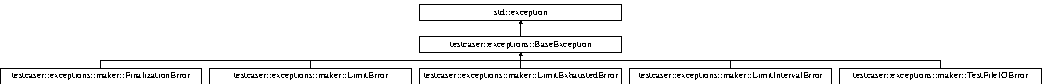
\includegraphics[height=1.135135cm]{classtestcaser_1_1exceptions_1_1BaseException}
\end{center}
\end{figure}
\subsection*{Public Member Functions}
\begin{DoxyCompactItemize}
\item 
\mbox{\hyperlink{classtestcaser_1_1exceptions_1_1BaseException_a70b5f42e6197e2600f7163f843060af2}{Base\+Exception}} (std\+::string reason)
\begin{DoxyCompactList}\small\item\em Construct a new Base Exception object. \end{DoxyCompactList}\item 
void \mbox{\hyperlink{classtestcaser_1_1exceptions_1_1BaseException_a92c371d40b0f3dbaa7de968ea67e5211}{set\+\_\+resolution}} (std\+::string resolution)
\begin{DoxyCompactList}\small\item\em Set the resolution string. \end{DoxyCompactList}\item 
virtual void \mbox{\hyperlink{classtestcaser_1_1exceptions_1_1BaseException_ad607ea04e2cb4ad9b8d0e2e6b6734f2f}{add\+\_\+more\+\_\+info}} ()=0
\begin{DoxyCompactList}\small\item\em A pure virtual function that must be overridden by decendants. \end{DoxyCompactList}\item 
virtual char const  $\ast$ \mbox{\hyperlink{classtestcaser_1_1exceptions_1_1BaseException_a28590a861913f870d9761990853e74b7}{what}} () const noexcept final override
\begin{DoxyCompactList}\small\item\em The final reason for the exception. \end{DoxyCompactList}\end{DoxyCompactItemize}
\subsection*{Protected Attributes}
\begin{DoxyCompactItemize}
\item 
std\+::string \mbox{\hyperlink{classtestcaser_1_1exceptions_1_1BaseException_abfc26d4451ae832886c32ad2e283104e}{more\+\_\+info}}
\begin{DoxyCompactList}\small\item\em more\+\_\+info contains more information about the Exception that shook the framework \end{DoxyCompactList}\end{DoxyCompactItemize}


\subsection{Detailed Description}
The Base Abstract exception class. All the Exceptions that will be thrown by the library will be inherited from this class. 



\subsection{Constructor \& Destructor Documentation}
\mbox{\Hypertarget{classtestcaser_1_1exceptions_1_1BaseException_a70b5f42e6197e2600f7163f843060af2}\label{classtestcaser_1_1exceptions_1_1BaseException_a70b5f42e6197e2600f7163f843060af2}} 
\index{testcaser::exceptions::BaseException@{testcaser::exceptions::BaseException}!BaseException@{BaseException}}
\index{BaseException@{BaseException}!testcaser::exceptions::BaseException@{testcaser::exceptions::BaseException}}
\subsubsection{\texorpdfstring{BaseException()}{BaseException()}}
{\footnotesize\ttfamily testcaser\+::exceptions\+::\+Base\+Exception\+::\+Base\+Exception (\begin{DoxyParamCaption}\item[{std\+::string}]{reason }\end{DoxyParamCaption})\hspace{0.3cm}{\ttfamily [inline]}}



Construct a new Base Exception object. 


\begin{DoxyParams}{Parameters}
{\em reason} & The message that will be carry forwarded to the \mbox{\hyperlink{classtestcaser_1_1exceptions_1_1BaseException_a28590a861913f870d9761990853e74b7}{what()}}. It usually specifies the reason of the exception \\
\hline
\end{DoxyParams}


\subsection{Member Function Documentation}
\mbox{\Hypertarget{classtestcaser_1_1exceptions_1_1BaseException_ad607ea04e2cb4ad9b8d0e2e6b6734f2f}\label{classtestcaser_1_1exceptions_1_1BaseException_ad607ea04e2cb4ad9b8d0e2e6b6734f2f}} 
\index{testcaser::exceptions::BaseException@{testcaser::exceptions::BaseException}!add\_more\_info@{add\_more\_info}}
\index{add\_more\_info@{add\_more\_info}!testcaser::exceptions::BaseException@{testcaser::exceptions::BaseException}}
\subsubsection{\texorpdfstring{add\_more\_info()}{add\_more\_info()}}
{\footnotesize\ttfamily virtual void testcaser\+::exceptions\+::\+Base\+Exception\+::add\+\_\+more\+\_\+info (\begin{DoxyParamCaption}{ }\end{DoxyParamCaption})\hspace{0.3cm}{\ttfamily [pure virtual]}}



A pure virtual function that must be overridden by decendants. 



Implemented in \mbox{\hyperlink{classtestcaser_1_1exceptions_1_1maker_1_1LimitExhaustedError_a40beeee091c1d5a35a12d6ab974c0895}{testcaser\+::exceptions\+::maker\+::\+Limit\+Exhausted\+Error}}, \mbox{\hyperlink{classtestcaser_1_1exceptions_1_1maker_1_1FinalizationError_a2e0aee4c53427abcbbcf3d5704687d76}{testcaser\+::exceptions\+::maker\+::\+Finalization\+Error}}, \mbox{\hyperlink{classtestcaser_1_1exceptions_1_1maker_1_1LimitIntervalError_a6a050ee23517e8dcb6477011b4a5e406}{testcaser\+::exceptions\+::maker\+::\+Limit\+Interval\+Error}}, \mbox{\hyperlink{classtestcaser_1_1exceptions_1_1maker_1_1TestFileIOError_ab83e748d26f860c9b045535447a383c5}{testcaser\+::exceptions\+::maker\+::\+Test\+File\+I\+O\+Error}}, and \mbox{\hyperlink{classtestcaser_1_1exceptions_1_1maker_1_1LimitError_adb0f0c92f0d78b26f4310301f97bff3a}{testcaser\+::exceptions\+::maker\+::\+Limit\+Error}}.

\mbox{\Hypertarget{classtestcaser_1_1exceptions_1_1BaseException_a92c371d40b0f3dbaa7de968ea67e5211}\label{classtestcaser_1_1exceptions_1_1BaseException_a92c371d40b0f3dbaa7de968ea67e5211}} 
\index{testcaser::exceptions::BaseException@{testcaser::exceptions::BaseException}!set\_resolution@{set\_resolution}}
\index{set\_resolution@{set\_resolution}!testcaser::exceptions::BaseException@{testcaser::exceptions::BaseException}}
\subsubsection{\texorpdfstring{set\_resolution()}{set\_resolution()}}
{\footnotesize\ttfamily void testcaser\+::exceptions\+::\+Base\+Exception\+::set\+\_\+resolution (\begin{DoxyParamCaption}\item[{std\+::string}]{resolution }\end{DoxyParamCaption})\hspace{0.3cm}{\ttfamily [inline]}}



Set the resolution string. 


\begin{DoxyParams}{Parameters}
{\em resolution} & If this error is generic and can be resolved. Help user with tips to fix this fatal exception \\
\hline
\end{DoxyParams}
\mbox{\Hypertarget{classtestcaser_1_1exceptions_1_1BaseException_a28590a861913f870d9761990853e74b7}\label{classtestcaser_1_1exceptions_1_1BaseException_a28590a861913f870d9761990853e74b7}} 
\index{testcaser::exceptions::BaseException@{testcaser::exceptions::BaseException}!what@{what}}
\index{what@{what}!testcaser::exceptions::BaseException@{testcaser::exceptions::BaseException}}
\subsubsection{\texorpdfstring{what()}{what()}}
{\footnotesize\ttfamily virtual char const$\ast$ testcaser\+::exceptions\+::\+Base\+Exception\+::what (\begin{DoxyParamCaption}{ }\end{DoxyParamCaption}) const\hspace{0.3cm}{\ttfamily [inline]}, {\ttfamily [final]}, {\ttfamily [override]}, {\ttfamily [virtual]}, {\ttfamily [noexcept]}}



The final reason for the exception. 

\begin{DoxyReturn}{Returns}
const char$\ast$ The message of the exception 
\end{DoxyReturn}


\subsection{Member Data Documentation}
\mbox{\Hypertarget{classtestcaser_1_1exceptions_1_1BaseException_abfc26d4451ae832886c32ad2e283104e}\label{classtestcaser_1_1exceptions_1_1BaseException_abfc26d4451ae832886c32ad2e283104e}} 
\index{testcaser::exceptions::BaseException@{testcaser::exceptions::BaseException}!more\_info@{more\_info}}
\index{more\_info@{more\_info}!testcaser::exceptions::BaseException@{testcaser::exceptions::BaseException}}
\subsubsection{\texorpdfstring{more\_info}{more\_info}}
{\footnotesize\ttfamily std\+::string testcaser\+::exceptions\+::\+Base\+Exception\+::more\+\_\+info\hspace{0.3cm}{\ttfamily [protected]}}



more\+\_\+info contains more information about the Exception that shook the framework 



The documentation for this class was generated from the following file\+:\begin{DoxyCompactItemize}
\item 
testcaser/core/exceptions/Base\+Exceptions.\+hpp\end{DoxyCompactItemize}

\hypertarget{structtestcaser_1_1internal_1_1executor__engine}{}\section{testcaser\+:\+:internal\+:\+:executor\+\_\+engine Struct Reference}
\label{structtestcaser_1_1internal_1_1executor__engine}\index{testcaser::internal::executor\_engine@{testcaser::internal::executor\_engine}}


Engine that is responsible for running and benchmarking the binary on the given input and constraint.  




{\ttfamily \#include $<$executor.\+hpp$>$}

\subsection*{Static Public Member Functions}
\begin{DoxyCompactItemize}
\item 
static \mbox{\hyperlink{classtestcaser_1_1integrator_1_1Result}{testcaser\+::integrator\+::\+Result}} \mbox{\hyperlink{structtestcaser_1_1internal_1_1executor__engine_a51f467bc2013c188b5e4454fa919ea70}{for\+\_\+execution\+\_\+of}} (std\+::string bin, std\+::string in, std\+::string out, size\+\_\+t mem, size\+\_\+t tim, size\+\_\+t auto\+\_\+exit\+\_\+wait, bool auto\+\_\+exit)
\begin{DoxyCompactList}\small\item\em starts the execution of the new child process with all the arguments \end{DoxyCompactList}\item 
static double \mbox{\hyperlink{structtestcaser_1_1internal_1_1executor__engine_af3546e4b21e46fc05bb38f014a88ed6f}{current\+\_\+high\+\_\+precision\+\_\+time}} ()
\begin{DoxyCompactList}\small\item\em Returns the current wall time with microsecond precision. \end{DoxyCompactList}\item 
static int \mbox{\hyperlink{structtestcaser_1_1internal_1_1executor__engine_ab70c6b9356bc0dbaf138aa017b048e8a}{get\+\_\+virtual\+\_\+memory\+\_\+use}} (pid\+\_\+t pid)
\begin{DoxyCompactList}\small\item\em Get the virtual memory used by the pid specified. \end{DoxyCompactList}\item 
static int \mbox{\hyperlink{structtestcaser_1_1internal_1_1executor__engine_a7162cc64fce4440e029086bf4f1efc7f}{get\+\_\+physical\+\_\+memory\+\_\+use}} (pid\+\_\+t pid)
\begin{DoxyCompactList}\small\item\em Get the physical memory used by the pid specified. \end{DoxyCompactList}\item 
static int \mbox{\hyperlink{structtestcaser_1_1internal_1_1executor__engine_a80ed3584cab00a573de09502df329919}{parse}} (char $\ast$line)
\begin{DoxyCompactList}\small\item\em Parses the line to extract virtual memory use. \end{DoxyCompactList}\item 
static bool \mbox{\hyperlink{structtestcaser_1_1internal_1_1executor__engine_a3649324b1da2b5fc41627ca7a73135f4}{is\+\_\+readable\+\_\+file}} (std\+::string file)
\begin{DoxyCompactList}\small\item\em shows if file is readable in text mode. \end{DoxyCompactList}\item 
static bool \mbox{\hyperlink{structtestcaser_1_1internal_1_1executor__engine_ac4add5efeeecea04a65f06c5f32f62fe}{is\+\_\+readable\+\_\+binary}} (std\+::string file)
\begin{DoxyCompactList}\small\item\em shows if file is readable in binary mode. \end{DoxyCompactList}\end{DoxyCompactItemize}


\subsection{Detailed Description}
Engine that is responsible for running and benchmarking the binary on the given input and constraint. 

\subsection{Member Function Documentation}
\mbox{\Hypertarget{structtestcaser_1_1internal_1_1executor__engine_af3546e4b21e46fc05bb38f014a88ed6f}\label{structtestcaser_1_1internal_1_1executor__engine_af3546e4b21e46fc05bb38f014a88ed6f}} 
\index{testcaser::internal::executor\_engine@{testcaser::internal::executor\_engine}!current\_high\_precision\_time@{current\_high\_precision\_time}}
\index{current\_high\_precision\_time@{current\_high\_precision\_time}!testcaser::internal::executor\_engine@{testcaser::internal::executor\_engine}}
\subsubsection{\texorpdfstring{current\_high\_precision\_time()}{current\_high\_precision\_time()}}
{\footnotesize\ttfamily static double testcaser\+::internal\+::executor\+\_\+engine\+::current\+\_\+high\+\_\+precision\+\_\+time (\begin{DoxyParamCaption}{ }\end{DoxyParamCaption})\hspace{0.3cm}{\ttfamily [inline]}, {\ttfamily [static]}}



Returns the current wall time with microsecond precision. 

\begin{DoxyReturn}{Returns}
double the current time. 
\end{DoxyReturn}
\mbox{\Hypertarget{structtestcaser_1_1internal_1_1executor__engine_a51f467bc2013c188b5e4454fa919ea70}\label{structtestcaser_1_1internal_1_1executor__engine_a51f467bc2013c188b5e4454fa919ea70}} 
\index{testcaser::internal::executor\_engine@{testcaser::internal::executor\_engine}!for\_execution\_of@{for\_execution\_of}}
\index{for\_execution\_of@{for\_execution\_of}!testcaser::internal::executor\_engine@{testcaser::internal::executor\_engine}}
\subsubsection{\texorpdfstring{for\_execution\_of()}{for\_execution\_of()}}
{\footnotesize\ttfamily static \mbox{\hyperlink{classtestcaser_1_1integrator_1_1Result}{testcaser\+::integrator\+::\+Result}} testcaser\+::internal\+::executor\+\_\+engine\+::for\+\_\+execution\+\_\+of (\begin{DoxyParamCaption}\item[{std\+::string}]{bin,  }\item[{std\+::string}]{in,  }\item[{std\+::string}]{out,  }\item[{size\+\_\+t}]{mem,  }\item[{size\+\_\+t}]{tim,  }\item[{size\+\_\+t}]{auto\+\_\+exit\+\_\+wait,  }\item[{bool}]{auto\+\_\+exit }\end{DoxyParamCaption})\hspace{0.3cm}{\ttfamily [inline]}, {\ttfamily [static]}}



starts the execution of the new child process with all the arguments 


\begin{DoxyParams}{Parameters}
{\em bin} & path of the executable to run in the child process. \\
\hline
{\em in} & path of the input file to provide to the binary \\
\hline
{\em out} & path of the output file to write binary\textquotesingle{}s output \\
\hline
{\em mem} & the memory limit of the binary \\
\hline
{\em tim} & the time limit of the binary in seconds \\
\hline
{\em auto\+\_\+exit\+\_\+wait} & if auto exit is false. How long should we wait before a S\+I\+G\+K\+I\+LL to kill the binary. \\
\hline
{\em auto\+\_\+exit} & should we exit the binary as soon as time or memory limit is passed? \\
\hline
\end{DoxyParams}
\begin{DoxyReturn}{Returns}
testcaser\+::integrator\+::\+Integration\+Result 
\end{DoxyReturn}
\mbox{\Hypertarget{structtestcaser_1_1internal_1_1executor__engine_a7162cc64fce4440e029086bf4f1efc7f}\label{structtestcaser_1_1internal_1_1executor__engine_a7162cc64fce4440e029086bf4f1efc7f}} 
\index{testcaser::internal::executor\_engine@{testcaser::internal::executor\_engine}!get\_physical\_memory\_use@{get\_physical\_memory\_use}}
\index{get\_physical\_memory\_use@{get\_physical\_memory\_use}!testcaser::internal::executor\_engine@{testcaser::internal::executor\_engine}}
\subsubsection{\texorpdfstring{get\_physical\_memory\_use()}{get\_physical\_memory\_use()}}
{\footnotesize\ttfamily static int testcaser\+::internal\+::executor\+\_\+engine\+::get\+\_\+physical\+\_\+memory\+\_\+use (\begin{DoxyParamCaption}\item[{pid\+\_\+t}]{pid }\end{DoxyParamCaption})\hspace{0.3cm}{\ttfamily [inline]}, {\ttfamily [static]}}



Get the physical memory used by the pid specified. 


\begin{DoxyParams}{Parameters}
{\em pid} & the pid of process to monitor \\
\hline
\end{DoxyParams}
\begin{DoxyReturn}{Returns}
int the memory used in KB 
\end{DoxyReturn}
\mbox{\Hypertarget{structtestcaser_1_1internal_1_1executor__engine_ab70c6b9356bc0dbaf138aa017b048e8a}\label{structtestcaser_1_1internal_1_1executor__engine_ab70c6b9356bc0dbaf138aa017b048e8a}} 
\index{testcaser::internal::executor\_engine@{testcaser::internal::executor\_engine}!get\_virtual\_memory\_use@{get\_virtual\_memory\_use}}
\index{get\_virtual\_memory\_use@{get\_virtual\_memory\_use}!testcaser::internal::executor\_engine@{testcaser::internal::executor\_engine}}
\subsubsection{\texorpdfstring{get\_virtual\_memory\_use()}{get\_virtual\_memory\_use()}}
{\footnotesize\ttfamily static int testcaser\+::internal\+::executor\+\_\+engine\+::get\+\_\+virtual\+\_\+memory\+\_\+use (\begin{DoxyParamCaption}\item[{pid\+\_\+t}]{pid }\end{DoxyParamCaption})\hspace{0.3cm}{\ttfamily [inline]}, {\ttfamily [static]}}



Get the virtual memory used by the pid specified. 


\begin{DoxyParams}{Parameters}
{\em pid} & the pid of process to monitor \\
\hline
\end{DoxyParams}
\begin{DoxyReturn}{Returns}
int the memory used in KB 
\end{DoxyReturn}
\mbox{\Hypertarget{structtestcaser_1_1internal_1_1executor__engine_ac4add5efeeecea04a65f06c5f32f62fe}\label{structtestcaser_1_1internal_1_1executor__engine_ac4add5efeeecea04a65f06c5f32f62fe}} 
\index{testcaser::internal::executor\_engine@{testcaser::internal::executor\_engine}!is\_readable\_binary@{is\_readable\_binary}}
\index{is\_readable\_binary@{is\_readable\_binary}!testcaser::internal::executor\_engine@{testcaser::internal::executor\_engine}}
\subsubsection{\texorpdfstring{is\_readable\_binary()}{is\_readable\_binary()}}
{\footnotesize\ttfamily static bool testcaser\+::internal\+::executor\+\_\+engine\+::is\+\_\+readable\+\_\+binary (\begin{DoxyParamCaption}\item[{std\+::string}]{file }\end{DoxyParamCaption})\hspace{0.3cm}{\ttfamily [inline]}, {\ttfamily [static]}}



shows if file is readable in binary mode. 


\begin{DoxyParams}{Parameters}
{\em file} & the file to check for \\
\hline
\end{DoxyParams}
\begin{DoxyReturn}{Returns}
true if file is readable in binary 

false if file is not readable in binary 
\end{DoxyReturn}
\mbox{\Hypertarget{structtestcaser_1_1internal_1_1executor__engine_a3649324b1da2b5fc41627ca7a73135f4}\label{structtestcaser_1_1internal_1_1executor__engine_a3649324b1da2b5fc41627ca7a73135f4}} 
\index{testcaser::internal::executor\_engine@{testcaser::internal::executor\_engine}!is\_readable\_file@{is\_readable\_file}}
\index{is\_readable\_file@{is\_readable\_file}!testcaser::internal::executor\_engine@{testcaser::internal::executor\_engine}}
\subsubsection{\texorpdfstring{is\_readable\_file()}{is\_readable\_file()}}
{\footnotesize\ttfamily static bool testcaser\+::internal\+::executor\+\_\+engine\+::is\+\_\+readable\+\_\+file (\begin{DoxyParamCaption}\item[{std\+::string}]{file }\end{DoxyParamCaption})\hspace{0.3cm}{\ttfamily [inline]}, {\ttfamily [static]}}



shows if file is readable in text mode. 


\begin{DoxyParams}{Parameters}
{\em file} & the file to check for \\
\hline
\end{DoxyParams}
\begin{DoxyReturn}{Returns}
true if file is readable in text 

false if file is not readable in text 
\end{DoxyReturn}
\mbox{\Hypertarget{structtestcaser_1_1internal_1_1executor__engine_a80ed3584cab00a573de09502df329919}\label{structtestcaser_1_1internal_1_1executor__engine_a80ed3584cab00a573de09502df329919}} 
\index{testcaser::internal::executor\_engine@{testcaser::internal::executor\_engine}!parse@{parse}}
\index{parse@{parse}!testcaser::internal::executor\_engine@{testcaser::internal::executor\_engine}}
\subsubsection{\texorpdfstring{parse()}{parse()}}
{\footnotesize\ttfamily static int testcaser\+::internal\+::executor\+\_\+engine\+::parse (\begin{DoxyParamCaption}\item[{char $\ast$}]{line }\end{DoxyParamCaption})\hspace{0.3cm}{\ttfamily [inline]}, {\ttfamily [static]}}



Parses the line to extract virtual memory use. 


\begin{DoxyParams}{Parameters}
{\em line} & the line to extract info from \\
\hline
\end{DoxyParams}
\begin{DoxyReturn}{Returns}
int the vm use in KB 
\end{DoxyReturn}


The documentation for this struct was generated from the following file\+:\begin{DoxyCompactItemize}
\item 
testcaser/core/integrator/engine/executor.\+hpp\end{DoxyCompactItemize}

\hypertarget{classtestcaser_1_1exceptions_1_1maker_1_1FinalizationError}{}\section{testcaser\+:\+:exceptions\+:\+:maker\+:\+:Finalization\+Error Class Reference}
\label{classtestcaser_1_1exceptions_1_1maker_1_1FinalizationError}\index{testcaser::exceptions::maker::FinalizationError@{testcaser::exceptions::maker::FinalizationError}}


Exception that is thrown when a finalized builder is modified with add\+\_\+line(..)  




{\ttfamily \#include $<$Build\+Exception.\+hpp$>$}

Inheritance diagram for testcaser\+:\+:exceptions\+:\+:maker\+:\+:Finalization\+Error\+:\begin{figure}[H]
\begin{center}
\leavevmode
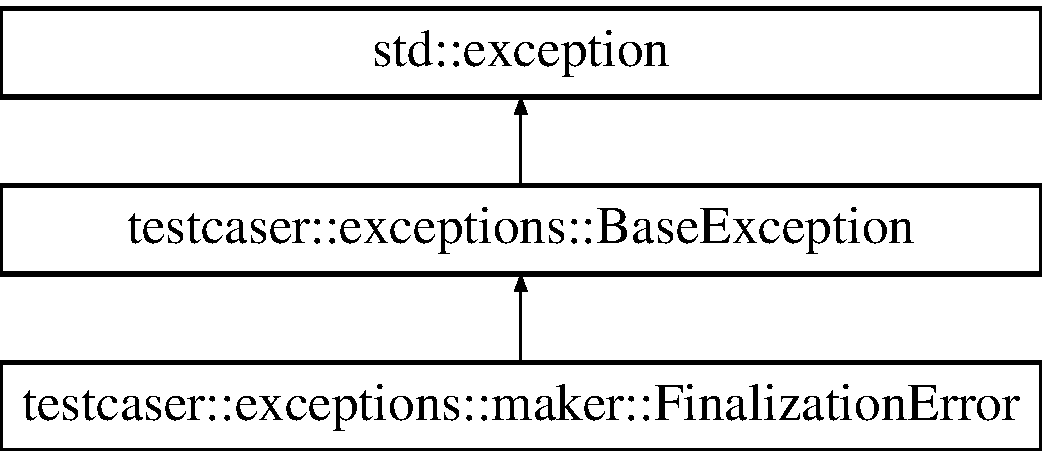
\includegraphics[height=3.000000cm]{classtestcaser_1_1exceptions_1_1maker_1_1FinalizationError}
\end{center}
\end{figure}
\subsection*{Public Member Functions}
\begin{DoxyCompactItemize}
\item 
\mbox{\hyperlink{classtestcaser_1_1exceptions_1_1maker_1_1FinalizationError_a0f878eb50c25b123675bc01eb66fd3bd}{Finalization\+Error}} (std\+::string details)
\begin{DoxyCompactList}\small\item\em Construct a new Finalization Error object. \end{DoxyCompactList}\item 
void \mbox{\hyperlink{classtestcaser_1_1exceptions_1_1maker_1_1FinalizationError_a2e0aee4c53427abcbbcf3d5704687d76}{add\+\_\+more\+\_\+info}} () final override
\begin{DoxyCompactList}\small\item\em Extra details that shows the state that caused the exception. \end{DoxyCompactList}\end{DoxyCompactItemize}
\subsection*{Additional Inherited Members}


\subsection{Detailed Description}
Exception that is thrown when a finalized builder is modified with add\+\_\+line(..) 



\subsection{Constructor \& Destructor Documentation}
\mbox{\Hypertarget{classtestcaser_1_1exceptions_1_1maker_1_1FinalizationError_a0f878eb50c25b123675bc01eb66fd3bd}\label{classtestcaser_1_1exceptions_1_1maker_1_1FinalizationError_a0f878eb50c25b123675bc01eb66fd3bd}} 
\index{testcaser::exceptions::maker::FinalizationError@{testcaser::exceptions::maker::FinalizationError}!FinalizationError@{FinalizationError}}
\index{FinalizationError@{FinalizationError}!testcaser::exceptions::maker::FinalizationError@{testcaser::exceptions::maker::FinalizationError}}
\subsubsection{\texorpdfstring{FinalizationError()}{FinalizationError()}}
{\footnotesize\ttfamily testcaser\+::exceptions\+::maker\+::\+Finalization\+Error\+::\+Finalization\+Error (\begin{DoxyParamCaption}\item[{std\+::string}]{details }\end{DoxyParamCaption})\hspace{0.3cm}{\ttfamily [inline]}}



Construct a new Finalization Error object. 


\begin{DoxyParams}{Parameters}
{\em details} & Generic message to show to use for the exception \\
\hline
\end{DoxyParams}


\subsection{Member Function Documentation}
\mbox{\Hypertarget{classtestcaser_1_1exceptions_1_1maker_1_1FinalizationError_a2e0aee4c53427abcbbcf3d5704687d76}\label{classtestcaser_1_1exceptions_1_1maker_1_1FinalizationError_a2e0aee4c53427abcbbcf3d5704687d76}} 
\index{testcaser::exceptions::maker::FinalizationError@{testcaser::exceptions::maker::FinalizationError}!add\_more\_info@{add\_more\_info}}
\index{add\_more\_info@{add\_more\_info}!testcaser::exceptions::maker::FinalizationError@{testcaser::exceptions::maker::FinalizationError}}
\subsubsection{\texorpdfstring{add\_more\_info()}{add\_more\_info()}}
{\footnotesize\ttfamily void testcaser\+::exceptions\+::maker\+::\+Finalization\+Error\+::add\+\_\+more\+\_\+info (\begin{DoxyParamCaption}{ }\end{DoxyParamCaption})\hspace{0.3cm}{\ttfamily [inline]}, {\ttfamily [final]}, {\ttfamily [override]}, {\ttfamily [virtual]}}



Extra details that shows the state that caused the exception. 



Implements \mbox{\hyperlink{classtestcaser_1_1exceptions_1_1BaseException_ad607ea04e2cb4ad9b8d0e2e6b6734f2f}{testcaser\+::exceptions\+::\+Base\+Exception}}.



The documentation for this class was generated from the following file\+:\begin{DoxyCompactItemize}
\item 
testcaser/core/exceptions/Build\+Exception.\+hpp\end{DoxyCompactItemize}

\hypertarget{structtestcaser_1_1maker_1_1limits_1_1Intervals}{}\section{testcaser\+:\+:maker\+:\+:limits\+:\+:Intervals$<$ T $>$ Struct Template Reference}
\label{structtestcaser_1_1maker_1_1limits_1_1Intervals}\index{testcaser\+::maker\+::limits\+::\+Intervals$<$ T $>$@{testcaser\+::maker\+::limits\+::\+Intervals$<$ T $>$}}


Interval holding class. Interval is \mbox{[}lower, upper) type.  




{\ttfamily \#include $<$limits.\+hpp$>$}

\subsection*{Public Member Functions}
\begin{DoxyCompactItemize}
\item 
\hyperlink{structtestcaser_1_1maker_1_1limits_1_1Intervals_a69fe886908002aa20f41ed886fc213ef}{Intervals} (T a, T b)
\begin{DoxyCompactList}\small\item\em Construct a new \hyperlink{structtestcaser_1_1maker_1_1limits_1_1Intervals}{Intervals} object. \end{DoxyCompactList}\item 
\hyperlink{structtestcaser_1_1maker_1_1limits_1_1Intervals_ad899dc031cbffd5247b9b39e23577a52}{Intervals} (std\+::pair$<$ T, T $>$ pp)
\begin{DoxyCompactList}\small\item\em Construct a new \hyperlink{structtestcaser_1_1maker_1_1limits_1_1Intervals}{Intervals} object. \end{DoxyCompactList}\item 
bool \hyperlink{structtestcaser_1_1maker_1_1limits_1_1Intervals_a68c68c86d5074b2853d0f8582381fc7a}{operator$<$} (const \hyperlink{structtestcaser_1_1maker_1_1limits_1_1Intervals}{Intervals} \&that) const
\begin{DoxyCompactList}\small\item\em compares two interval from their starting/lower points \end{DoxyCompactList}\item 
bool \hyperlink{structtestcaser_1_1maker_1_1limits_1_1Intervals_af5204b4a6f57b16d6719a16554321b4b}{operator$>$} (const \hyperlink{structtestcaser_1_1maker_1_1limits_1_1Intervals}{Intervals} \&that) const
\begin{DoxyCompactList}\small\item\em compares two interval from their starting/lower points \end{DoxyCompactList}\end{DoxyCompactItemize}
\subsection*{Public Attributes}
\begin{DoxyCompactItemize}
\item 
\mbox{\Hypertarget{structtestcaser_1_1maker_1_1limits_1_1Intervals_ae8f8bf8607c83b429729bd36e74699dd}\label{structtestcaser_1_1maker_1_1limits_1_1Intervals_ae8f8bf8607c83b429729bd36e74699dd}} 
T \hyperlink{structtestcaser_1_1maker_1_1limits_1_1Intervals_ae8f8bf8607c83b429729bd36e74699dd}{upper}
\begin{DoxyCompactList}\small\item\em upper the upper limit \end{DoxyCompactList}\item 
\mbox{\Hypertarget{structtestcaser_1_1maker_1_1limits_1_1Intervals_a51f277024599c24b6bfdffe1276f236d}\label{structtestcaser_1_1maker_1_1limits_1_1Intervals_a51f277024599c24b6bfdffe1276f236d}} 
T \hyperlink{structtestcaser_1_1maker_1_1limits_1_1Intervals_a51f277024599c24b6bfdffe1276f236d}{lower}
\begin{DoxyCompactList}\small\item\em lower the lower limit of the interval \end{DoxyCompactList}\end{DoxyCompactItemize}


\subsection{Detailed Description}
\subsubsection*{template$<$class T$>$\newline
struct testcaser\+::maker\+::limits\+::\+Intervals$<$ T $>$}

Interval holding class. Interval is \mbox{[}lower, upper) type. 


\begin{DoxyTemplParams}{Template Parameters}
{\em T} & The lower and upper limit type \\
\hline
\end{DoxyTemplParams}


\subsection{Constructor \& Destructor Documentation}
\mbox{\Hypertarget{structtestcaser_1_1maker_1_1limits_1_1Intervals_a69fe886908002aa20f41ed886fc213ef}\label{structtestcaser_1_1maker_1_1limits_1_1Intervals_a69fe886908002aa20f41ed886fc213ef}} 
\index{testcaser\+::maker\+::limits\+::\+Intervals@{testcaser\+::maker\+::limits\+::\+Intervals}!Intervals@{Intervals}}
\index{Intervals@{Intervals}!testcaser\+::maker\+::limits\+::\+Intervals@{testcaser\+::maker\+::limits\+::\+Intervals}}
\subsubsection{\texorpdfstring{Intervals()}{Intervals()}\hspace{0.1cm}{\footnotesize\ttfamily [1/2]}}
{\footnotesize\ttfamily template$<$class T$>$ \\
\hyperlink{structtestcaser_1_1maker_1_1limits_1_1Intervals}{testcaser\+::maker\+::limits\+::\+Intervals}$<$ T $>$\+::\hyperlink{structtestcaser_1_1maker_1_1limits_1_1Intervals}{Intervals} (\begin{DoxyParamCaption}\item[{T}]{a,  }\item[{T}]{b }\end{DoxyParamCaption})\hspace{0.3cm}{\ttfamily [inline]}}



Construct a new \hyperlink{structtestcaser_1_1maker_1_1limits_1_1Intervals}{Intervals} object. 


\begin{DoxyParams}{Parameters}
{\em a} & Lower limit of interval \\
\hline
{\em b} & Upper limit of the interval \\
\hline
\end{DoxyParams}
\mbox{\Hypertarget{structtestcaser_1_1maker_1_1limits_1_1Intervals_ad899dc031cbffd5247b9b39e23577a52}\label{structtestcaser_1_1maker_1_1limits_1_1Intervals_ad899dc031cbffd5247b9b39e23577a52}} 
\index{testcaser\+::maker\+::limits\+::\+Intervals@{testcaser\+::maker\+::limits\+::\+Intervals}!Intervals@{Intervals}}
\index{Intervals@{Intervals}!testcaser\+::maker\+::limits\+::\+Intervals@{testcaser\+::maker\+::limits\+::\+Intervals}}
\subsubsection{\texorpdfstring{Intervals()}{Intervals()}\hspace{0.1cm}{\footnotesize\ttfamily [2/2]}}
{\footnotesize\ttfamily template$<$class T$>$ \\
\hyperlink{structtestcaser_1_1maker_1_1limits_1_1Intervals}{testcaser\+::maker\+::limits\+::\+Intervals}$<$ T $>$\+::\hyperlink{structtestcaser_1_1maker_1_1limits_1_1Intervals}{Intervals} (\begin{DoxyParamCaption}\item[{std\+::pair$<$ T, T $>$}]{pp }\end{DoxyParamCaption})\hspace{0.3cm}{\ttfamily [inline]}}



Construct a new \hyperlink{structtestcaser_1_1maker_1_1limits_1_1Intervals}{Intervals} object. 


\begin{DoxyParams}{Parameters}
{\em pp} & An Interval as a pair of with first being the lower and second being the higher interval limit \\
\hline
\end{DoxyParams}


\subsection{Member Function Documentation}
\mbox{\Hypertarget{structtestcaser_1_1maker_1_1limits_1_1Intervals_a68c68c86d5074b2853d0f8582381fc7a}\label{structtestcaser_1_1maker_1_1limits_1_1Intervals_a68c68c86d5074b2853d0f8582381fc7a}} 
\index{testcaser\+::maker\+::limits\+::\+Intervals@{testcaser\+::maker\+::limits\+::\+Intervals}!operator$<$@{operator$<$}}
\index{operator$<$@{operator$<$}!testcaser\+::maker\+::limits\+::\+Intervals@{testcaser\+::maker\+::limits\+::\+Intervals}}
\subsubsection{\texorpdfstring{operator$<$()}{operator<()}}
{\footnotesize\ttfamily template$<$class T$>$ \\
bool \hyperlink{structtestcaser_1_1maker_1_1limits_1_1Intervals}{testcaser\+::maker\+::limits\+::\+Intervals}$<$ T $>$\+::operator$<$ (\begin{DoxyParamCaption}\item[{const \hyperlink{structtestcaser_1_1maker_1_1limits_1_1Intervals}{Intervals}$<$ T $>$ \&}]{that }\end{DoxyParamCaption}) const\hspace{0.3cm}{\ttfamily [inline]}}



compares two interval from their starting/lower points 


\begin{DoxyParams}{Parameters}
{\em that} & other object to compare with \\
\hline
\end{DoxyParams}
\begin{DoxyReturn}{Returns}
true if the other\textquotesingle{}s lower limit is bigger that this lower limit 

false otherwise 
\end{DoxyReturn}
\mbox{\Hypertarget{structtestcaser_1_1maker_1_1limits_1_1Intervals_af5204b4a6f57b16d6719a16554321b4b}\label{structtestcaser_1_1maker_1_1limits_1_1Intervals_af5204b4a6f57b16d6719a16554321b4b}} 
\index{testcaser\+::maker\+::limits\+::\+Intervals@{testcaser\+::maker\+::limits\+::\+Intervals}!operator$>$@{operator$>$}}
\index{operator$>$@{operator$>$}!testcaser\+::maker\+::limits\+::\+Intervals@{testcaser\+::maker\+::limits\+::\+Intervals}}
\subsubsection{\texorpdfstring{operator$>$()}{operator>()}}
{\footnotesize\ttfamily template$<$class T$>$ \\
bool \hyperlink{structtestcaser_1_1maker_1_1limits_1_1Intervals}{testcaser\+::maker\+::limits\+::\+Intervals}$<$ T $>$\+::operator$>$ (\begin{DoxyParamCaption}\item[{const \hyperlink{structtestcaser_1_1maker_1_1limits_1_1Intervals}{Intervals}$<$ T $>$ \&}]{that }\end{DoxyParamCaption}) const\hspace{0.3cm}{\ttfamily [inline]}}



compares two interval from their starting/lower points 


\begin{DoxyParams}{Parameters}
{\em that} & other object to compare with \\
\hline
\end{DoxyParams}
\begin{DoxyReturn}{Returns}
true if the this lower limit is bigger that that\textquotesingle{}s lower limit 

false otherwise 
\end{DoxyReturn}


The documentation for this struct was generated from the following file\+:\begin{DoxyCompactItemize}
\item 
testcaser/core/maker/randoms/limits.\+hpp\end{DoxyCompactItemize}

\hypertarget{classtestcaser_1_1exceptions_1_1maker_1_1LimitError}{}\section{testcaser\+:\+:exceptions\+:\+:maker\+:\+:Limit\+Error Class Reference}
\label{classtestcaser_1_1exceptions_1_1maker_1_1LimitError}\index{testcaser::exceptions::maker::LimitError@{testcaser::exceptions::maker::LimitError}}


Exception that is raised when an invalid limit is given to any Random class.  




{\ttfamily \#include $<$Invalid\+Limit.\+hpp$>$}

Inheritance diagram for testcaser\+:\+:exceptions\+:\+:maker\+:\+:Limit\+Error\+:\begin{figure}[H]
\begin{center}
\leavevmode
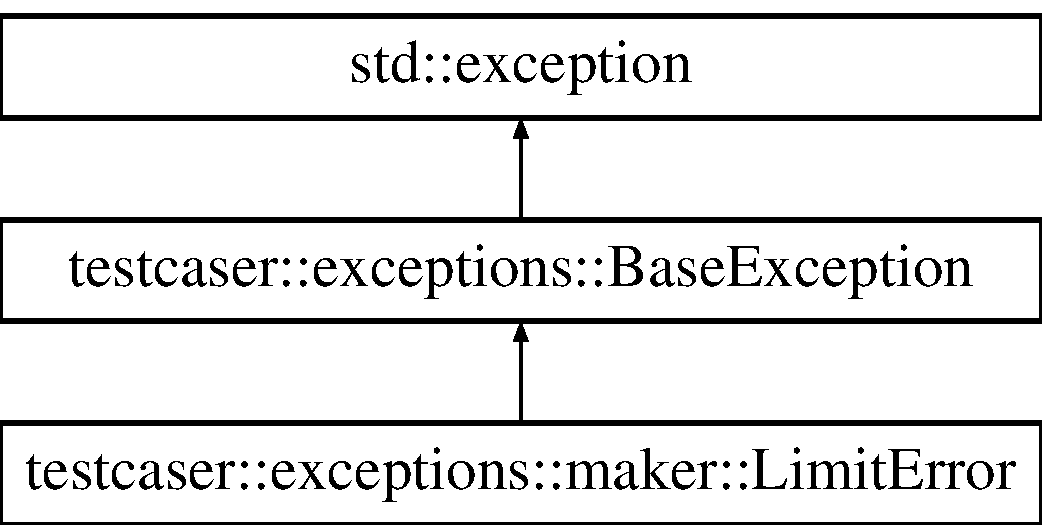
\includegraphics[height=3.000000cm]{classtestcaser_1_1exceptions_1_1maker_1_1LimitError}
\end{center}
\end{figure}
\subsection*{Public Member Functions}
\begin{DoxyCompactItemize}
\item 
\mbox{\hyperlink{classtestcaser_1_1exceptions_1_1maker_1_1LimitError_a93442165f498e8910b4c2170a05d3b3a}{Limit\+Error}} (std\+::string details)
\begin{DoxyCompactList}\small\item\em Construct a new Limit Error object. \end{DoxyCompactList}\item 
void \mbox{\hyperlink{classtestcaser_1_1exceptions_1_1maker_1_1LimitError_adb0f0c92f0d78b26f4310301f97bff3a}{add\+\_\+more\+\_\+info}} () final override
\begin{DoxyCompactList}\small\item\em The Error message that will be shown to the user that explains the actual state of the exception. \end{DoxyCompactList}\end{DoxyCompactItemize}
\subsection*{Additional Inherited Members}


\subsection{Detailed Description}
Exception that is raised when an invalid limit is given to any Random class. 



\subsection{Constructor \& Destructor Documentation}
\mbox{\Hypertarget{classtestcaser_1_1exceptions_1_1maker_1_1LimitError_a93442165f498e8910b4c2170a05d3b3a}\label{classtestcaser_1_1exceptions_1_1maker_1_1LimitError_a93442165f498e8910b4c2170a05d3b3a}} 
\index{testcaser::exceptions::maker::LimitError@{testcaser::exceptions::maker::LimitError}!LimitError@{LimitError}}
\index{LimitError@{LimitError}!testcaser::exceptions::maker::LimitError@{testcaser::exceptions::maker::LimitError}}
\subsubsection{\texorpdfstring{LimitError()}{LimitError()}}
{\footnotesize\ttfamily testcaser\+::exceptions\+::maker\+::\+Limit\+Error\+::\+Limit\+Error (\begin{DoxyParamCaption}\item[{std\+::string}]{details }\end{DoxyParamCaption})\hspace{0.3cm}{\ttfamily [inline]}}



Construct a new Limit Error object. 


\begin{DoxyParams}{Parameters}
{\em details} & The Generic Error type message \\
\hline
\end{DoxyParams}


\subsection{Member Function Documentation}
\mbox{\Hypertarget{classtestcaser_1_1exceptions_1_1maker_1_1LimitError_adb0f0c92f0d78b26f4310301f97bff3a}\label{classtestcaser_1_1exceptions_1_1maker_1_1LimitError_adb0f0c92f0d78b26f4310301f97bff3a}} 
\index{testcaser::exceptions::maker::LimitError@{testcaser::exceptions::maker::LimitError}!add\_more\_info@{add\_more\_info}}
\index{add\_more\_info@{add\_more\_info}!testcaser::exceptions::maker::LimitError@{testcaser::exceptions::maker::LimitError}}
\subsubsection{\texorpdfstring{add\_more\_info()}{add\_more\_info()}}
{\footnotesize\ttfamily void testcaser\+::exceptions\+::maker\+::\+Limit\+Error\+::add\+\_\+more\+\_\+info (\begin{DoxyParamCaption}{ }\end{DoxyParamCaption})\hspace{0.3cm}{\ttfamily [inline]}, {\ttfamily [final]}, {\ttfamily [override]}, {\ttfamily [virtual]}}



The Error message that will be shown to the user that explains the actual state of the exception. 



Implements \mbox{\hyperlink{classtestcaser_1_1exceptions_1_1BaseException_ad607ea04e2cb4ad9b8d0e2e6b6734f2f}{testcaser\+::exceptions\+::\+Base\+Exception}}.



The documentation for this class was generated from the following file\+:\begin{DoxyCompactItemize}
\item 
core/exceptions/Invalid\+Limit.\+hpp\end{DoxyCompactItemize}

\hypertarget{classtestcaser_1_1exceptions_1_1maker_1_1LimitExhaustedError}{}\section{testcaser\+:\+:exceptions\+:\+:maker\+:\+:Limit\+Exhausted\+Error Class Reference}
\label{classtestcaser_1_1exceptions_1_1maker_1_1LimitExhaustedError}\index{testcaser::exceptions::maker::LimitExhaustedError@{testcaser::exceptions::maker::LimitExhaustedError}}


Exception that is thrown when all interval exceptions have exhaused the limit size.  




{\ttfamily \#include $<$Invalid\+Limit.\+hpp$>$}

Inheritance diagram for testcaser\+:\+:exceptions\+:\+:maker\+:\+:Limit\+Exhausted\+Error\+:\begin{figure}[H]
\begin{center}
\leavevmode
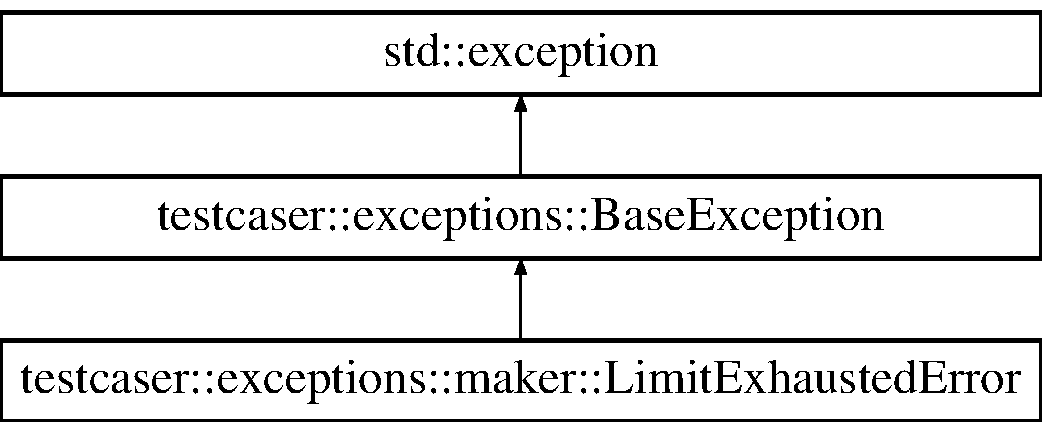
\includegraphics[height=3.000000cm]{classtestcaser_1_1exceptions_1_1maker_1_1LimitExhaustedError}
\end{center}
\end{figure}
\subsection*{Public Member Functions}
\begin{DoxyCompactItemize}
\item 
\mbox{\hyperlink{classtestcaser_1_1exceptions_1_1maker_1_1LimitExhaustedError_a9ba2ad6f34755e1039132a7fa763e55f}{Limit\+Exhausted\+Error}} (std\+::string details)
\begin{DoxyCompactList}\small\item\em Construct a new Limit Exhausted Error object. \end{DoxyCompactList}\item 
void \mbox{\hyperlink{classtestcaser_1_1exceptions_1_1maker_1_1LimitExhaustedError_a40beeee091c1d5a35a12d6ab974c0895}{add\+\_\+more\+\_\+info}} () final override
\begin{DoxyCompactList}\small\item\em More information about the state in which exception was raised. \end{DoxyCompactList}\end{DoxyCompactItemize}
\subsection*{Additional Inherited Members}


\subsection{Detailed Description}
Exception that is thrown when all interval exceptions have exhaused the limit size. 



\subsection{Constructor \& Destructor Documentation}
\mbox{\Hypertarget{classtestcaser_1_1exceptions_1_1maker_1_1LimitExhaustedError_a9ba2ad6f34755e1039132a7fa763e55f}\label{classtestcaser_1_1exceptions_1_1maker_1_1LimitExhaustedError_a9ba2ad6f34755e1039132a7fa763e55f}} 
\index{testcaser::exceptions::maker::LimitExhaustedError@{testcaser::exceptions::maker::LimitExhaustedError}!LimitExhaustedError@{LimitExhaustedError}}
\index{LimitExhaustedError@{LimitExhaustedError}!testcaser::exceptions::maker::LimitExhaustedError@{testcaser::exceptions::maker::LimitExhaustedError}}
\subsubsection{\texorpdfstring{LimitExhaustedError()}{LimitExhaustedError()}}
{\footnotesize\ttfamily testcaser\+::exceptions\+::maker\+::\+Limit\+Exhausted\+Error\+::\+Limit\+Exhausted\+Error (\begin{DoxyParamCaption}\item[{std\+::string}]{details }\end{DoxyParamCaption})\hspace{0.3cm}{\ttfamily [inline]}}



Construct a new Limit Exhausted Error object. 


\begin{DoxyParams}{Parameters}
{\em details} & The Genric message for the exception \\
\hline
\end{DoxyParams}


\subsection{Member Function Documentation}
\mbox{\Hypertarget{classtestcaser_1_1exceptions_1_1maker_1_1LimitExhaustedError_a40beeee091c1d5a35a12d6ab974c0895}\label{classtestcaser_1_1exceptions_1_1maker_1_1LimitExhaustedError_a40beeee091c1d5a35a12d6ab974c0895}} 
\index{testcaser::exceptions::maker::LimitExhaustedError@{testcaser::exceptions::maker::LimitExhaustedError}!add\_more\_info@{add\_more\_info}}
\index{add\_more\_info@{add\_more\_info}!testcaser::exceptions::maker::LimitExhaustedError@{testcaser::exceptions::maker::LimitExhaustedError}}
\subsubsection{\texorpdfstring{add\_more\_info()}{add\_more\_info()}}
{\footnotesize\ttfamily void testcaser\+::exceptions\+::maker\+::\+Limit\+Exhausted\+Error\+::add\+\_\+more\+\_\+info (\begin{DoxyParamCaption}{ }\end{DoxyParamCaption})\hspace{0.3cm}{\ttfamily [inline]}, {\ttfamily [final]}, {\ttfamily [override]}, {\ttfamily [virtual]}}



More information about the state in which exception was raised. 



Implements \mbox{\hyperlink{classtestcaser_1_1exceptions_1_1BaseException_ad607ea04e2cb4ad9b8d0e2e6b6734f2f}{testcaser\+::exceptions\+::\+Base\+Exception}}.



The documentation for this class was generated from the following file\+:\begin{DoxyCompactItemize}
\item 
testcaser/core/exceptions/Invalid\+Limit.\+hpp\end{DoxyCompactItemize}

\hypertarget{classtestcaser_1_1exceptions_1_1maker_1_1LimitIntervalError}{}\section{testcaser\+:\+:exceptions\+:\+:maker\+:\+:Limit\+Interval\+Error Class Reference}
\label{classtestcaser_1_1exceptions_1_1maker_1_1LimitIntervalError}\index{testcaser::exceptions::maker::LimitIntervalError@{testcaser::exceptions::maker::LimitIntervalError}}


Exception that is raised when an Interval setting to limits are ambigious.  




{\ttfamily \#include $<$Invalid\+Limit.\+hpp$>$}

Inheritance diagram for testcaser\+:\+:exceptions\+:\+:maker\+:\+:Limit\+Interval\+Error\+:\begin{figure}[H]
\begin{center}
\leavevmode
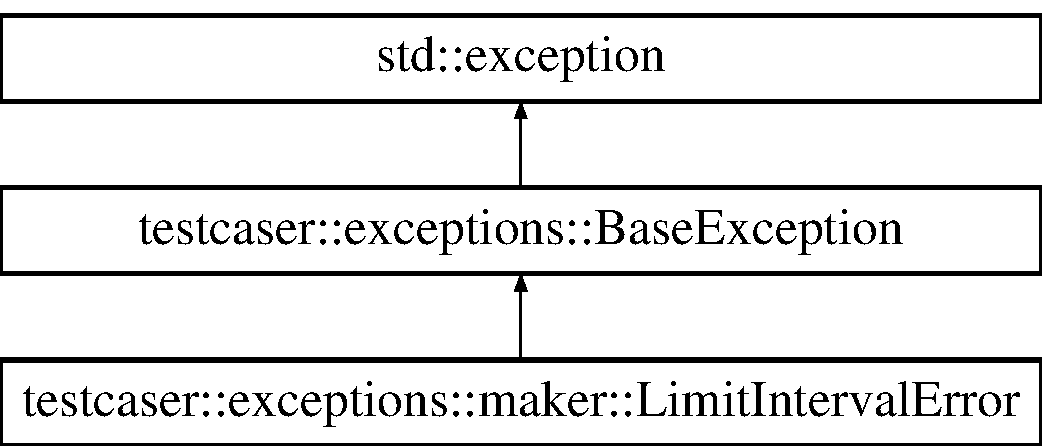
\includegraphics[height=3.000000cm]{classtestcaser_1_1exceptions_1_1maker_1_1LimitIntervalError}
\end{center}
\end{figure}
\subsection*{Public Member Functions}
\begin{DoxyCompactItemize}
\item 
\mbox{\hyperlink{classtestcaser_1_1exceptions_1_1maker_1_1LimitIntervalError_aa25b5fb862cea4c6946ee334cb7590eb}{Limit\+Interval\+Error}} (std\+::string details)
\begin{DoxyCompactList}\small\item\em Construct a new Limit Interval Error object. \end{DoxyCompactList}\item 
void \mbox{\hyperlink{classtestcaser_1_1exceptions_1_1maker_1_1LimitIntervalError_a6a050ee23517e8dcb6477011b4a5e406}{add\+\_\+more\+\_\+info}} () final override
\begin{DoxyCompactList}\small\item\em Adds more information that explains the stat of the exception. \end{DoxyCompactList}\end{DoxyCompactItemize}
\subsection*{Additional Inherited Members}


\subsection{Detailed Description}
Exception that is raised when an Interval setting to limits are ambigious. 



\subsection{Constructor \& Destructor Documentation}
\mbox{\Hypertarget{classtestcaser_1_1exceptions_1_1maker_1_1LimitIntervalError_aa25b5fb862cea4c6946ee334cb7590eb}\label{classtestcaser_1_1exceptions_1_1maker_1_1LimitIntervalError_aa25b5fb862cea4c6946ee334cb7590eb}} 
\index{testcaser::exceptions::maker::LimitIntervalError@{testcaser::exceptions::maker::LimitIntervalError}!LimitIntervalError@{LimitIntervalError}}
\index{LimitIntervalError@{LimitIntervalError}!testcaser::exceptions::maker::LimitIntervalError@{testcaser::exceptions::maker::LimitIntervalError}}
\subsubsection{\texorpdfstring{LimitIntervalError()}{LimitIntervalError()}}
{\footnotesize\ttfamily testcaser\+::exceptions\+::maker\+::\+Limit\+Interval\+Error\+::\+Limit\+Interval\+Error (\begin{DoxyParamCaption}\item[{std\+::string}]{details }\end{DoxyParamCaption})\hspace{0.3cm}{\ttfamily [inline]}}



Construct a new Limit Interval Error object. 


\begin{DoxyParams}{Parameters}
{\em details} & The Generic message type for the excpetion \\
\hline
\end{DoxyParams}


\subsection{Member Function Documentation}
\mbox{\Hypertarget{classtestcaser_1_1exceptions_1_1maker_1_1LimitIntervalError_a6a050ee23517e8dcb6477011b4a5e406}\label{classtestcaser_1_1exceptions_1_1maker_1_1LimitIntervalError_a6a050ee23517e8dcb6477011b4a5e406}} 
\index{testcaser::exceptions::maker::LimitIntervalError@{testcaser::exceptions::maker::LimitIntervalError}!add\_more\_info@{add\_more\_info}}
\index{add\_more\_info@{add\_more\_info}!testcaser::exceptions::maker::LimitIntervalError@{testcaser::exceptions::maker::LimitIntervalError}}
\subsubsection{\texorpdfstring{add\_more\_info()}{add\_more\_info()}}
{\footnotesize\ttfamily void testcaser\+::exceptions\+::maker\+::\+Limit\+Interval\+Error\+::add\+\_\+more\+\_\+info (\begin{DoxyParamCaption}{ }\end{DoxyParamCaption})\hspace{0.3cm}{\ttfamily [inline]}, {\ttfamily [final]}, {\ttfamily [override]}, {\ttfamily [virtual]}}



Adds more information that explains the stat of the exception. 



Implements \mbox{\hyperlink{classtestcaser_1_1exceptions_1_1BaseException_ad607ea04e2cb4ad9b8d0e2e6b6734f2f}{testcaser\+::exceptions\+::\+Base\+Exception}}.



The documentation for this class was generated from the following file\+:\begin{DoxyCompactItemize}
\item 
testcaser/core/exceptions/Invalid\+Limit.\+hpp\end{DoxyCompactItemize}

\hypertarget{classtestcaser_1_1maker_1_1types_1_1RandomAlphabet}{}\section{testcaser\+:\+:maker\+:\+:types\+:\+:Random\+Alphabet$<$ Generator, Distribution $>$ Class Template Reference}
\label{classtestcaser_1_1maker_1_1types_1_1RandomAlphabet}\index{testcaser::maker::types::RandomAlphabet$<$ Generator, Distribution $>$@{testcaser::maker::types::RandomAlphabet$<$ Generator, Distribution $>$}}


\mbox{\hyperlink{classtestcaser_1_1maker_1_1types_1_1RandomAlphabet}{Random\+Alphabet}} object generates a random alphabet every time .\mbox{\hyperlink{classtestcaser_1_1maker_1_1types_1_1RandomAlphabet_a6498f1e44b84cb66c1c1dc6de642b218}{get()}} is called it follows the generator and the distribution type that you provide.  




{\ttfamily \#include $<$Random\+Types.\+hpp$>$}

\subsection*{Public Member Functions}
\begin{DoxyCompactItemize}
\item 
\mbox{\hyperlink{classtestcaser_1_1maker_1_1types_1_1RandomAlphabet_ab4cab36c953e73837f726215309577ba}{Random\+Alphabet}} ()
\begin{DoxyCompactList}\small\item\em Construct a new Random Alphabet object. \end{DoxyCompactList}\item 
char \mbox{\hyperlink{classtestcaser_1_1maker_1_1types_1_1RandomAlphabet_a6fccb771852c1f44ed268a9867589026}{get\+\_\+lower}} () const
\begin{DoxyCompactList}\small\item\em Get the lower case character. \end{DoxyCompactList}\item 
char \mbox{\hyperlink{classtestcaser_1_1maker_1_1types_1_1RandomAlphabet_a398a597e207dea4a284537feb8fc6086}{get\+\_\+upper}} () const
\begin{DoxyCompactList}\small\item\em Get the upper case char. \end{DoxyCompactList}\item 
char \mbox{\hyperlink{classtestcaser_1_1maker_1_1types_1_1RandomAlphabet_a6498f1e44b84cb66c1c1dc6de642b218}{get}} () const
\begin{DoxyCompactList}\small\item\em returns a distribution based character from mix of upper and lower \end{DoxyCompactList}\end{DoxyCompactItemize}


\subsection{Detailed Description}
\subsubsection*{template$<$class Generator = std\+::mt19937, class Distribution = std\+::uniform\+\_\+int\+\_\+distribution$<$unsigned long long$>$$>$\newline
class testcaser\+::maker\+::types\+::\+Random\+Alphabet$<$ Generator, Distribution $>$}

\mbox{\hyperlink{classtestcaser_1_1maker_1_1types_1_1RandomAlphabet}{Random\+Alphabet}} object generates a random alphabet every time .\mbox{\hyperlink{classtestcaser_1_1maker_1_1types_1_1RandomAlphabet_a6498f1e44b84cb66c1c1dc6de642b218}{get()}} is called it follows the generator and the distribution type that you provide. 


\begin{DoxyTemplParams}{Template Parameters}
{\em std\+::mt19937} & the random number generator to use \\
\hline
{\em std\+::uniform\+\_\+int\+\_\+distribution$<$unsigned} & long long$>$ the distribution to use to sample the random number \\
\hline
\end{DoxyTemplParams}


\subsection{Constructor \& Destructor Documentation}
\mbox{\Hypertarget{classtestcaser_1_1maker_1_1types_1_1RandomAlphabet_ab4cab36c953e73837f726215309577ba}\label{classtestcaser_1_1maker_1_1types_1_1RandomAlphabet_ab4cab36c953e73837f726215309577ba}} 
\index{testcaser::maker::types::RandomAlphabet$<$ Generator, Distribution $>$@{testcaser::maker::types::RandomAlphabet$<$ Generator, Distribution $>$}!RandomAlphabet@{RandomAlphabet}}
\index{RandomAlphabet@{RandomAlphabet}!testcaser::maker::types::RandomAlphabet$<$ Generator, Distribution $>$@{testcaser::maker::types::RandomAlphabet$<$ Generator, Distribution $>$}}
\subsubsection{\texorpdfstring{RandomAlphabet()}{RandomAlphabet()}}
{\footnotesize\ttfamily template$<$class Generator = std\+::mt19937, class Distribution = std\+::uniform\+\_\+int\+\_\+distribution$<$unsigned long long$>$$>$ \\
\mbox{\hyperlink{classtestcaser_1_1maker_1_1types_1_1RandomAlphabet}{testcaser\+::maker\+::types\+::\+Random\+Alphabet}}$<$ Generator, Distribution $>$\+::\mbox{\hyperlink{classtestcaser_1_1maker_1_1types_1_1RandomAlphabet}{Random\+Alphabet}} (\begin{DoxyParamCaption}{ }\end{DoxyParamCaption})\hspace{0.3cm}{\ttfamily [inline]}}



Construct a new Random Alphabet object. 



\subsection{Member Function Documentation}
\mbox{\Hypertarget{classtestcaser_1_1maker_1_1types_1_1RandomAlphabet_a6498f1e44b84cb66c1c1dc6de642b218}\label{classtestcaser_1_1maker_1_1types_1_1RandomAlphabet_a6498f1e44b84cb66c1c1dc6de642b218}} 
\index{testcaser::maker::types::RandomAlphabet$<$ Generator, Distribution $>$@{testcaser::maker::types::RandomAlphabet$<$ Generator, Distribution $>$}!get@{get}}
\index{get@{get}!testcaser::maker::types::RandomAlphabet$<$ Generator, Distribution $>$@{testcaser::maker::types::RandomAlphabet$<$ Generator, Distribution $>$}}
\subsubsection{\texorpdfstring{get()}{get()}}
{\footnotesize\ttfamily template$<$class Generator = std\+::mt19937, class Distribution = std\+::uniform\+\_\+int\+\_\+distribution$<$unsigned long long$>$$>$ \\
char \mbox{\hyperlink{classtestcaser_1_1maker_1_1types_1_1RandomAlphabet}{testcaser\+::maker\+::types\+::\+Random\+Alphabet}}$<$ Generator, Distribution $>$\+::get (\begin{DoxyParamCaption}{ }\end{DoxyParamCaption}) const\hspace{0.3cm}{\ttfamily [inline]}}



returns a distribution based character from mix of upper and lower 

\begin{DoxyReturn}{Returns}
char a valid upper or lower character 
\end{DoxyReturn}
\mbox{\Hypertarget{classtestcaser_1_1maker_1_1types_1_1RandomAlphabet_a6fccb771852c1f44ed268a9867589026}\label{classtestcaser_1_1maker_1_1types_1_1RandomAlphabet_a6fccb771852c1f44ed268a9867589026}} 
\index{testcaser::maker::types::RandomAlphabet$<$ Generator, Distribution $>$@{testcaser::maker::types::RandomAlphabet$<$ Generator, Distribution $>$}!get\_lower@{get\_lower}}
\index{get\_lower@{get\_lower}!testcaser::maker::types::RandomAlphabet$<$ Generator, Distribution $>$@{testcaser::maker::types::RandomAlphabet$<$ Generator, Distribution $>$}}
\subsubsection{\texorpdfstring{get\_lower()}{get\_lower()}}
{\footnotesize\ttfamily template$<$class Generator = std\+::mt19937, class Distribution = std\+::uniform\+\_\+int\+\_\+distribution$<$unsigned long long$>$$>$ \\
char \mbox{\hyperlink{classtestcaser_1_1maker_1_1types_1_1RandomAlphabet}{testcaser\+::maker\+::types\+::\+Random\+Alphabet}}$<$ Generator, Distribution $>$\+::get\+\_\+lower (\begin{DoxyParamCaption}{ }\end{DoxyParamCaption}) const\hspace{0.3cm}{\ttfamily [inline]}}



Get the lower case character. 

\begin{DoxyReturn}{Returns}
char the lower case char 
\end{DoxyReturn}
\mbox{\Hypertarget{classtestcaser_1_1maker_1_1types_1_1RandomAlphabet_a398a597e207dea4a284537feb8fc6086}\label{classtestcaser_1_1maker_1_1types_1_1RandomAlphabet_a398a597e207dea4a284537feb8fc6086}} 
\index{testcaser::maker::types::RandomAlphabet$<$ Generator, Distribution $>$@{testcaser::maker::types::RandomAlphabet$<$ Generator, Distribution $>$}!get\_upper@{get\_upper}}
\index{get\_upper@{get\_upper}!testcaser::maker::types::RandomAlphabet$<$ Generator, Distribution $>$@{testcaser::maker::types::RandomAlphabet$<$ Generator, Distribution $>$}}
\subsubsection{\texorpdfstring{get\_upper()}{get\_upper()}}
{\footnotesize\ttfamily template$<$class Generator = std\+::mt19937, class Distribution = std\+::uniform\+\_\+int\+\_\+distribution$<$unsigned long long$>$$>$ \\
char \mbox{\hyperlink{classtestcaser_1_1maker_1_1types_1_1RandomAlphabet}{testcaser\+::maker\+::types\+::\+Random\+Alphabet}}$<$ Generator, Distribution $>$\+::get\+\_\+upper (\begin{DoxyParamCaption}{ }\end{DoxyParamCaption}) const\hspace{0.3cm}{\ttfamily [inline]}}



Get the upper case char. 

\begin{DoxyReturn}{Returns}
char the upper case character 
\end{DoxyReturn}


The documentation for this class was generated from the following file\+:\begin{DoxyCompactItemize}
\item 
testcaser/core/maker/randoms/Random\+Types.\+hpp\end{DoxyCompactItemize}

\hypertarget{structtestcaser_1_1maker_1_1types_1_1RandomBinary}{}\section{testcaser\+:\+:maker\+:\+:types\+:\+:Random\+Binary$<$ Generator, Distribution $>$ Struct Template Reference}
\label{structtestcaser_1_1maker_1_1types_1_1RandomBinary}\index{testcaser::maker::types::RandomBinary$<$ Generator, Distribution $>$@{testcaser::maker::types::RandomBinary$<$ Generator, Distribution $>$}}


\mbox{\hyperlink{structtestcaser_1_1maker_1_1types_1_1RandomBinary}{Random\+Binary}} object generates a random binary every time .get() is called it follows the generator and the distribution type that you provide.  




{\ttfamily \#include $<$Random\+Types.\+hpp$>$}

\subsection*{Public Member Functions}
\begin{DoxyCompactItemize}
\item 
\mbox{\hyperlink{structtestcaser_1_1maker_1_1types_1_1RandomBinary_a6d3f045cf7406fcedfa1d1188194f7a8}{Random\+Binary}} ()
\begin{DoxyCompactList}\small\item\em Construct a new Random Binary object. \end{DoxyCompactList}\item 
bool \mbox{\hyperlink{structtestcaser_1_1maker_1_1types_1_1RandomBinary_a469154b51a27681c713c8b93ec1626b5}{get\+\_\+as\+\_\+boolean}} ()
\begin{DoxyCompactList}\small\item\em Get the random value as boolean object. \end{DoxyCompactList}\item 
unsigned long long \mbox{\hyperlink{structtestcaser_1_1maker_1_1types_1_1RandomBinary_a40519ce9d13d4e3681d4eeada57fbfb2}{get\+\_\+as\+\_\+int}} () const
\begin{DoxyCompactList}\small\item\em Get the random value as int object. \end{DoxyCompactList}\end{DoxyCompactItemize}
\subsection*{Public Attributes}
\begin{DoxyCompactItemize}
\item 
\mbox{\hyperlink{classtestcaser_1_1maker_1_1types_1_1RandomUnsignedInteger}{Random\+Unsigned\+Integer}}$<$ Generator, Distribution $>$ \mbox{\hyperlink{structtestcaser_1_1maker_1_1types_1_1RandomBinary_a387cd99ad534bb762a37e931a227925e}{rui}}
\begin{DoxyCompactList}\small\item\em rui the \mbox{\hyperlink{classtestcaser_1_1maker_1_1types_1_1RandomUnsignedInteger}{Random\+Unsigned\+Integer}} object to generate binary numbers with binary limit \end{DoxyCompactList}\end{DoxyCompactItemize}


\subsection{Detailed Description}
\subsubsection*{template$<$class Generator = std\+::mt19937, class Distribution = std\+::uniform\+\_\+int\+\_\+distribution$<$unsigned long long$>$$>$\newline
struct testcaser\+::maker\+::types\+::\+Random\+Binary$<$ Generator, Distribution $>$}

\mbox{\hyperlink{structtestcaser_1_1maker_1_1types_1_1RandomBinary}{Random\+Binary}} object generates a random binary every time .get() is called it follows the generator and the distribution type that you provide. 


\begin{DoxyTemplParams}{Template Parameters}
{\em std\+::mt19937} & the random number generator to use \\
\hline
{\em std\+::uniform\+\_\+int\+\_\+distribution$<$unsigned} & long long$>$ the distribution to use to sample the random number \\
\hline
\end{DoxyTemplParams}


\subsection{Constructor \& Destructor Documentation}
\mbox{\Hypertarget{structtestcaser_1_1maker_1_1types_1_1RandomBinary_a6d3f045cf7406fcedfa1d1188194f7a8}\label{structtestcaser_1_1maker_1_1types_1_1RandomBinary_a6d3f045cf7406fcedfa1d1188194f7a8}} 
\index{testcaser::maker::types::RandomBinary$<$ Generator, Distribution $>$@{testcaser::maker::types::RandomBinary$<$ Generator, Distribution $>$}!RandomBinary@{RandomBinary}}
\index{RandomBinary@{RandomBinary}!testcaser::maker::types::RandomBinary$<$ Generator, Distribution $>$@{testcaser::maker::types::RandomBinary$<$ Generator, Distribution $>$}}
\subsubsection{\texorpdfstring{RandomBinary()}{RandomBinary()}}
{\footnotesize\ttfamily template$<$class Generator = std\+::mt19937, class Distribution = std\+::uniform\+\_\+int\+\_\+distribution$<$unsigned long long$>$$>$ \\
\mbox{\hyperlink{structtestcaser_1_1maker_1_1types_1_1RandomBinary}{testcaser\+::maker\+::types\+::\+Random\+Binary}}$<$ Generator, Distribution $>$\+::\mbox{\hyperlink{structtestcaser_1_1maker_1_1types_1_1RandomBinary}{Random\+Binary}} (\begin{DoxyParamCaption}{ }\end{DoxyParamCaption})\hspace{0.3cm}{\ttfamily [inline]}}



Construct a new Random Binary object. 



\subsection{Member Function Documentation}
\mbox{\Hypertarget{structtestcaser_1_1maker_1_1types_1_1RandomBinary_a469154b51a27681c713c8b93ec1626b5}\label{structtestcaser_1_1maker_1_1types_1_1RandomBinary_a469154b51a27681c713c8b93ec1626b5}} 
\index{testcaser::maker::types::RandomBinary$<$ Generator, Distribution $>$@{testcaser::maker::types::RandomBinary$<$ Generator, Distribution $>$}!get\_as\_boolean@{get\_as\_boolean}}
\index{get\_as\_boolean@{get\_as\_boolean}!testcaser::maker::types::RandomBinary$<$ Generator, Distribution $>$@{testcaser::maker::types::RandomBinary$<$ Generator, Distribution $>$}}
\subsubsection{\texorpdfstring{get\_as\_boolean()}{get\_as\_boolean()}}
{\footnotesize\ttfamily template$<$class Generator = std\+::mt19937, class Distribution = std\+::uniform\+\_\+int\+\_\+distribution$<$unsigned long long$>$$>$ \\
bool \mbox{\hyperlink{structtestcaser_1_1maker_1_1types_1_1RandomBinary}{testcaser\+::maker\+::types\+::\+Random\+Binary}}$<$ Generator, Distribution $>$\+::get\+\_\+as\+\_\+boolean (\begin{DoxyParamCaption}{ }\end{DoxyParamCaption})\hspace{0.3cm}{\ttfamily [inline]}}



Get the random value as boolean object. 

\begin{DoxyReturn}{Returns}
true 

false 
\end{DoxyReturn}
\mbox{\Hypertarget{structtestcaser_1_1maker_1_1types_1_1RandomBinary_a40519ce9d13d4e3681d4eeada57fbfb2}\label{structtestcaser_1_1maker_1_1types_1_1RandomBinary_a40519ce9d13d4e3681d4eeada57fbfb2}} 
\index{testcaser::maker::types::RandomBinary$<$ Generator, Distribution $>$@{testcaser::maker::types::RandomBinary$<$ Generator, Distribution $>$}!get\_as\_int@{get\_as\_int}}
\index{get\_as\_int@{get\_as\_int}!testcaser::maker::types::RandomBinary$<$ Generator, Distribution $>$@{testcaser::maker::types::RandomBinary$<$ Generator, Distribution $>$}}
\subsubsection{\texorpdfstring{get\_as\_int()}{get\_as\_int()}}
{\footnotesize\ttfamily template$<$class Generator = std\+::mt19937, class Distribution = std\+::uniform\+\_\+int\+\_\+distribution$<$unsigned long long$>$$>$ \\
unsigned long long \mbox{\hyperlink{structtestcaser_1_1maker_1_1types_1_1RandomBinary}{testcaser\+::maker\+::types\+::\+Random\+Binary}}$<$ Generator, Distribution $>$\+::get\+\_\+as\+\_\+int (\begin{DoxyParamCaption}{ }\end{DoxyParamCaption}) const\hspace{0.3cm}{\ttfamily [inline]}}



Get the random value as int object. 

\begin{DoxyReturn}{Returns}
unsigned long long 
\end{DoxyReturn}


\subsection{Member Data Documentation}
\mbox{\Hypertarget{structtestcaser_1_1maker_1_1types_1_1RandomBinary_a387cd99ad534bb762a37e931a227925e}\label{structtestcaser_1_1maker_1_1types_1_1RandomBinary_a387cd99ad534bb762a37e931a227925e}} 
\index{testcaser::maker::types::RandomBinary$<$ Generator, Distribution $>$@{testcaser::maker::types::RandomBinary$<$ Generator, Distribution $>$}!rui@{rui}}
\index{rui@{rui}!testcaser::maker::types::RandomBinary$<$ Generator, Distribution $>$@{testcaser::maker::types::RandomBinary$<$ Generator, Distribution $>$}}
\subsubsection{\texorpdfstring{rui}{rui}}
{\footnotesize\ttfamily template$<$class Generator = std\+::mt19937, class Distribution = std\+::uniform\+\_\+int\+\_\+distribution$<$unsigned long long$>$$>$ \\
\mbox{\hyperlink{classtestcaser_1_1maker_1_1types_1_1RandomUnsignedInteger}{Random\+Unsigned\+Integer}}$<$Generator, Distribution$>$ \mbox{\hyperlink{structtestcaser_1_1maker_1_1types_1_1RandomBinary}{testcaser\+::maker\+::types\+::\+Random\+Binary}}$<$ Generator, Distribution $>$\+::rui}



rui the \mbox{\hyperlink{classtestcaser_1_1maker_1_1types_1_1RandomUnsignedInteger}{Random\+Unsigned\+Integer}} object to generate binary numbers with binary limit 



The documentation for this struct was generated from the following file\+:\begin{DoxyCompactItemize}
\item 
testcaser/core/maker/randoms/Random\+Types.\+hpp\end{DoxyCompactItemize}

\hypertarget{classtestcaser_1_1maker_1_1RandomCharacterLimit}{}\section{testcaser\+:\+:maker\+:\+:Random\+Character\+Limit Class Reference}
\label{classtestcaser_1_1maker_1_1RandomCharacterLimit}\index{testcaser::maker::RandomCharacterLimit@{testcaser::maker::RandomCharacterLimit}}
\subsection*{Public Member Functions}
\begin{DoxyCompactItemize}
\item 
\mbox{\hyperlink{classtestcaser_1_1maker_1_1RandomCharacterLimit_a2ebd894bf7f536219bf7a917ed036c55}{Random\+Character\+Limit}} (std\+::initializer\+\_\+list$<$ int $>$ llmt)
\begin{DoxyCompactList}\small\item\em Construct a new Random Character Limit object. \end{DoxyCompactList}\item 
\mbox{\hyperlink{classtestcaser_1_1maker_1_1RandomCharacterLimit_a7a85c6420ec09f97e648f516a9bb68fd}{Random\+Character\+Limit}} (int upper, int lower)
\begin{DoxyCompactList}\small\item\em Construct a new Random Character Limit object. \end{DoxyCompactList}\item 
void \mbox{\hyperlink{classtestcaser_1_1maker_1_1RandomCharacterLimit_a9fac35205a15685a2ce671f9f38279ab}{add\+\_\+interval\+\_\+exception}} (std\+::pair$<$ int, int $>$ interval)
\begin{DoxyCompactList}\small\item\em Adds a interval exception in between the limit say. Original Limit are \mbox{[}a, b) and you want to skip some intervals in between say \mbox{[}c,d) such that c $>$= a and d $<$ b then you would call this method with std\+::pair$<$c,d$>$ \end{DoxyCompactList}\item 
int \mbox{\hyperlink{classtestcaser_1_1maker_1_1RandomCharacterLimit_a912c757f9c26f6ba3e3ec18db3c904c5}{actual\+\_\+limit\+\_\+size}} ()
\begin{DoxyCompactList}\small\item\em The limit size after excluding all the exceptions in between them. \end{DoxyCompactList}\item 
bool \mbox{\hyperlink{classtestcaser_1_1maker_1_1RandomCharacterLimit_a1b3f0a14a18aa307cf4a82f834393928}{valid\+\_\+output}} (int out) const
\begin{DoxyCompactList}\small\item\em checks if the a char is a valid as per the limit constraints with exception internals in mind. \end{DoxyCompactList}\item 
\mbox{\hyperlink{classtestcaser_1_1maker_1_1RandomCharacterLimit_a230a33b5d028fdef4a027f7c96663d32}{operator Random\+Unsigned\+Integer\+Limit}} ()
\begin{DoxyCompactList}\small\item\em Converts this object to an object of \mbox{\hyperlink{classtestcaser_1_1maker_1_1RandomUnsignedIntegerLimit}{Random\+Unsigned\+Integer\+Limit}}. \end{DoxyCompactList}\end{DoxyCompactItemize}
\subsection*{Static Public Member Functions}
\begin{DoxyCompactItemize}
\item 
static \mbox{\hyperlink{classtestcaser_1_1maker_1_1RandomCharacterLimit}{Random\+Character\+Limit}} \mbox{\hyperlink{classtestcaser_1_1maker_1_1RandomCharacterLimit_ae6e40c00b9225a88b0133c17d4b24f90}{lower\+\_\+case\+\_\+alphabet\+\_\+limit}} ()
\begin{DoxyCompactList}\small\item\em returns the limit of the lower case alphabets. \end{DoxyCompactList}\item 
static \mbox{\hyperlink{classtestcaser_1_1maker_1_1RandomCharacterLimit}{Random\+Character\+Limit}} \mbox{\hyperlink{classtestcaser_1_1maker_1_1RandomCharacterLimit_a7a0ee0690e97a27402faca09c6044aed}{upper\+\_\+case\+\_\+alphabet\+\_\+limit}} ()
\begin{DoxyCompactList}\small\item\em returns the upper case alphabet limit \end{DoxyCompactList}\item 
static \mbox{\hyperlink{classtestcaser_1_1maker_1_1RandomCharacterLimit}{Random\+Character\+Limit}} \mbox{\hyperlink{classtestcaser_1_1maker_1_1RandomCharacterLimit_a4519263daf2737941039054c60c26ca5}{alphabet\+\_\+limit}} ()
\begin{DoxyCompactList}\small\item\em returns the mixed case alphabet limit \end{DoxyCompactList}\end{DoxyCompactItemize}
\subsection*{Public Attributes}
\begin{DoxyCompactItemize}
\item 
const int \mbox{\hyperlink{classtestcaser_1_1maker_1_1RandomCharacterLimit_adf6f29860db063472c941a169b918667}{Upper\+Limit}}
\begin{DoxyCompactList}\small\item\em Upper\+Limit the upper limit of the character as A\+S\+C\+II int. \end{DoxyCompactList}\item 
const int \mbox{\hyperlink{classtestcaser_1_1maker_1_1RandomCharacterLimit_a152f8b1958ceec1128967cefa40891d9}{Lower\+Limit}}
\begin{DoxyCompactList}\small\item\em Lower\+Limit the lower limit of the character as A\+S\+C\+II int. \end{DoxyCompactList}\end{DoxyCompactItemize}


\subsection{Constructor \& Destructor Documentation}
\mbox{\Hypertarget{classtestcaser_1_1maker_1_1RandomCharacterLimit_a2ebd894bf7f536219bf7a917ed036c55}\label{classtestcaser_1_1maker_1_1RandomCharacterLimit_a2ebd894bf7f536219bf7a917ed036c55}} 
\index{testcaser::maker::RandomCharacterLimit@{testcaser::maker::RandomCharacterLimit}!RandomCharacterLimit@{RandomCharacterLimit}}
\index{RandomCharacterLimit@{RandomCharacterLimit}!testcaser::maker::RandomCharacterLimit@{testcaser::maker::RandomCharacterLimit}}
\subsubsection{\texorpdfstring{RandomCharacterLimit()}{RandomCharacterLimit()}\hspace{0.1cm}{\footnotesize\ttfamily [1/2]}}
{\footnotesize\ttfamily testcaser\+::maker\+::\+Random\+Character\+Limit\+::\+Random\+Character\+Limit (\begin{DoxyParamCaption}\item[{std\+::initializer\+\_\+list$<$ int $>$}]{llmt }\end{DoxyParamCaption})\hspace{0.3cm}{\ttfamily [inline]}}



Construct a new Random Character Limit object. 


\begin{DoxyParams}{Parameters}
{\em llmt} & the limit as initializer list \\
\hline
\end{DoxyParams}
\mbox{\Hypertarget{classtestcaser_1_1maker_1_1RandomCharacterLimit_a7a85c6420ec09f97e648f516a9bb68fd}\label{classtestcaser_1_1maker_1_1RandomCharacterLimit_a7a85c6420ec09f97e648f516a9bb68fd}} 
\index{testcaser::maker::RandomCharacterLimit@{testcaser::maker::RandomCharacterLimit}!RandomCharacterLimit@{RandomCharacterLimit}}
\index{RandomCharacterLimit@{RandomCharacterLimit}!testcaser::maker::RandomCharacterLimit@{testcaser::maker::RandomCharacterLimit}}
\subsubsection{\texorpdfstring{RandomCharacterLimit()}{RandomCharacterLimit()}\hspace{0.1cm}{\footnotesize\ttfamily [2/2]}}
{\footnotesize\ttfamily testcaser\+::maker\+::\+Random\+Character\+Limit\+::\+Random\+Character\+Limit (\begin{DoxyParamCaption}\item[{int}]{upper,  }\item[{int}]{lower }\end{DoxyParamCaption})\hspace{0.3cm}{\ttfamily [inline]}}



Construct a new Random Character Limit object. 


\begin{DoxyParams}{Parameters}
{\em upper} & the upper bound of the limit (not included) \\
\hline
{\em lower} & the lower bound of the limit (included) \\
\hline
\end{DoxyParams}


\subsection{Member Function Documentation}
\mbox{\Hypertarget{classtestcaser_1_1maker_1_1RandomCharacterLimit_a912c757f9c26f6ba3e3ec18db3c904c5}\label{classtestcaser_1_1maker_1_1RandomCharacterLimit_a912c757f9c26f6ba3e3ec18db3c904c5}} 
\index{testcaser::maker::RandomCharacterLimit@{testcaser::maker::RandomCharacterLimit}!actual\_limit\_size@{actual\_limit\_size}}
\index{actual\_limit\_size@{actual\_limit\_size}!testcaser::maker::RandomCharacterLimit@{testcaser::maker::RandomCharacterLimit}}
\subsubsection{\texorpdfstring{actual\_limit\_size()}{actual\_limit\_size()}}
{\footnotesize\ttfamily int testcaser\+::maker\+::\+Random\+Character\+Limit\+::actual\+\_\+limit\+\_\+size (\begin{DoxyParamCaption}{ }\end{DoxyParamCaption})\hspace{0.3cm}{\ttfamily [inline]}}



The limit size after excluding all the exceptions in between them. 

\begin{DoxyReturn}{Returns}
int the value of the limit size 
\end{DoxyReturn}
\mbox{\Hypertarget{classtestcaser_1_1maker_1_1RandomCharacterLimit_a9fac35205a15685a2ce671f9f38279ab}\label{classtestcaser_1_1maker_1_1RandomCharacterLimit_a9fac35205a15685a2ce671f9f38279ab}} 
\index{testcaser::maker::RandomCharacterLimit@{testcaser::maker::RandomCharacterLimit}!add\_interval\_exception@{add\_interval\_exception}}
\index{add\_interval\_exception@{add\_interval\_exception}!testcaser::maker::RandomCharacterLimit@{testcaser::maker::RandomCharacterLimit}}
\subsubsection{\texorpdfstring{add\_interval\_exception()}{add\_interval\_exception()}}
{\footnotesize\ttfamily void testcaser\+::maker\+::\+Random\+Character\+Limit\+::add\+\_\+interval\+\_\+exception (\begin{DoxyParamCaption}\item[{std\+::pair$<$ int, int $>$}]{interval }\end{DoxyParamCaption})\hspace{0.3cm}{\ttfamily [inline]}}



Adds a interval exception in between the limit say. Original Limit are \mbox{[}a, b) and you want to skip some intervals in between say \mbox{[}c,d) such that c $>$= a and d $<$ b then you would call this method with std\+::pair$<$c,d$>$ 


\begin{DoxyParams}{Parameters}
{\em interval} & the std\+::pair object holding an interval in between the original limit. \\
\hline
\end{DoxyParams}
\mbox{\Hypertarget{classtestcaser_1_1maker_1_1RandomCharacterLimit_a4519263daf2737941039054c60c26ca5}\label{classtestcaser_1_1maker_1_1RandomCharacterLimit_a4519263daf2737941039054c60c26ca5}} 
\index{testcaser::maker::RandomCharacterLimit@{testcaser::maker::RandomCharacterLimit}!alphabet\_limit@{alphabet\_limit}}
\index{alphabet\_limit@{alphabet\_limit}!testcaser::maker::RandomCharacterLimit@{testcaser::maker::RandomCharacterLimit}}
\subsubsection{\texorpdfstring{alphabet\_limit()}{alphabet\_limit()}}
{\footnotesize\ttfamily static \mbox{\hyperlink{classtestcaser_1_1maker_1_1RandomCharacterLimit}{Random\+Character\+Limit}} testcaser\+::maker\+::\+Random\+Character\+Limit\+::alphabet\+\_\+limit (\begin{DoxyParamCaption}{ }\end{DoxyParamCaption})\hspace{0.3cm}{\ttfamily [inline]}, {\ttfamily [static]}}



returns the mixed case alphabet limit 

\begin{DoxyReturn}{Returns}
\mbox{\hyperlink{classtestcaser_1_1maker_1_1RandomCharacterLimit}{Random\+Character\+Limit}} 
\end{DoxyReturn}
\mbox{\Hypertarget{classtestcaser_1_1maker_1_1RandomCharacterLimit_ae6e40c00b9225a88b0133c17d4b24f90}\label{classtestcaser_1_1maker_1_1RandomCharacterLimit_ae6e40c00b9225a88b0133c17d4b24f90}} 
\index{testcaser::maker::RandomCharacterLimit@{testcaser::maker::RandomCharacterLimit}!lower\_case\_alphabet\_limit@{lower\_case\_alphabet\_limit}}
\index{lower\_case\_alphabet\_limit@{lower\_case\_alphabet\_limit}!testcaser::maker::RandomCharacterLimit@{testcaser::maker::RandomCharacterLimit}}
\subsubsection{\texorpdfstring{lower\_case\_alphabet\_limit()}{lower\_case\_alphabet\_limit()}}
{\footnotesize\ttfamily static \mbox{\hyperlink{classtestcaser_1_1maker_1_1RandomCharacterLimit}{Random\+Character\+Limit}} testcaser\+::maker\+::\+Random\+Character\+Limit\+::lower\+\_\+case\+\_\+alphabet\+\_\+limit (\begin{DoxyParamCaption}{ }\end{DoxyParamCaption})\hspace{0.3cm}{\ttfamily [inline]}, {\ttfamily [static]}}



returns the limit of the lower case alphabets. 

\begin{DoxyReturn}{Returns}
\mbox{\hyperlink{classtestcaser_1_1maker_1_1RandomCharacterLimit}{Random\+Character\+Limit}} 
\end{DoxyReturn}
\mbox{\Hypertarget{classtestcaser_1_1maker_1_1RandomCharacterLimit_a230a33b5d028fdef4a027f7c96663d32}\label{classtestcaser_1_1maker_1_1RandomCharacterLimit_a230a33b5d028fdef4a027f7c96663d32}} 
\index{testcaser::maker::RandomCharacterLimit@{testcaser::maker::RandomCharacterLimit}!operator RandomUnsignedIntegerLimit@{operator RandomUnsignedIntegerLimit}}
\index{operator RandomUnsignedIntegerLimit@{operator RandomUnsignedIntegerLimit}!testcaser::maker::RandomCharacterLimit@{testcaser::maker::RandomCharacterLimit}}
\subsubsection{\texorpdfstring{operator RandomUnsignedIntegerLimit()}{operator RandomUnsignedIntegerLimit()}}
{\footnotesize\ttfamily testcaser\+::maker\+::\+Random\+Character\+Limit\+::operator \mbox{\hyperlink{classtestcaser_1_1maker_1_1RandomUnsignedIntegerLimit}{Random\+Unsigned\+Integer\+Limit}} (\begin{DoxyParamCaption}{ }\end{DoxyParamCaption})\hspace{0.3cm}{\ttfamily [inline]}}



Converts this object to an object of \mbox{\hyperlink{classtestcaser_1_1maker_1_1RandomUnsignedIntegerLimit}{Random\+Unsigned\+Integer\+Limit}}. 

\begin{DoxyReturn}{Returns}
\mbox{\hyperlink{classtestcaser_1_1maker_1_1RandomUnsignedIntegerLimit}{Random\+Unsigned\+Integer\+Limit}} 
\end{DoxyReturn}
\mbox{\Hypertarget{classtestcaser_1_1maker_1_1RandomCharacterLimit_a7a0ee0690e97a27402faca09c6044aed}\label{classtestcaser_1_1maker_1_1RandomCharacterLimit_a7a0ee0690e97a27402faca09c6044aed}} 
\index{testcaser::maker::RandomCharacterLimit@{testcaser::maker::RandomCharacterLimit}!upper\_case\_alphabet\_limit@{upper\_case\_alphabet\_limit}}
\index{upper\_case\_alphabet\_limit@{upper\_case\_alphabet\_limit}!testcaser::maker::RandomCharacterLimit@{testcaser::maker::RandomCharacterLimit}}
\subsubsection{\texorpdfstring{upper\_case\_alphabet\_limit()}{upper\_case\_alphabet\_limit()}}
{\footnotesize\ttfamily static \mbox{\hyperlink{classtestcaser_1_1maker_1_1RandomCharacterLimit}{Random\+Character\+Limit}} testcaser\+::maker\+::\+Random\+Character\+Limit\+::upper\+\_\+case\+\_\+alphabet\+\_\+limit (\begin{DoxyParamCaption}{ }\end{DoxyParamCaption})\hspace{0.3cm}{\ttfamily [inline]}, {\ttfamily [static]}}



returns the upper case alphabet limit 

\begin{DoxyReturn}{Returns}
\mbox{\hyperlink{classtestcaser_1_1maker_1_1RandomCharacterLimit}{Random\+Character\+Limit}} 
\end{DoxyReturn}
\mbox{\Hypertarget{classtestcaser_1_1maker_1_1RandomCharacterLimit_a1b3f0a14a18aa307cf4a82f834393928}\label{classtestcaser_1_1maker_1_1RandomCharacterLimit_a1b3f0a14a18aa307cf4a82f834393928}} 
\index{testcaser::maker::RandomCharacterLimit@{testcaser::maker::RandomCharacterLimit}!valid\_output@{valid\_output}}
\index{valid\_output@{valid\_output}!testcaser::maker::RandomCharacterLimit@{testcaser::maker::RandomCharacterLimit}}
\subsubsection{\texorpdfstring{valid\_output()}{valid\_output()}}
{\footnotesize\ttfamily bool testcaser\+::maker\+::\+Random\+Character\+Limit\+::valid\+\_\+output (\begin{DoxyParamCaption}\item[{int}]{out }\end{DoxyParamCaption}) const\hspace{0.3cm}{\ttfamily [inline]}}



checks if the a char is a valid as per the limit constraints with exception internals in mind. 


\begin{DoxyParams}{Parameters}
{\em out} & the value to check for \\
\hline
\end{DoxyParams}
\begin{DoxyReturn}{Returns}
true if doesn\textquotesingle{}t violates the limit rules 

false if violates any rule or is out of limit 
\end{DoxyReturn}


\subsection{Member Data Documentation}
\mbox{\Hypertarget{classtestcaser_1_1maker_1_1RandomCharacterLimit_a152f8b1958ceec1128967cefa40891d9}\label{classtestcaser_1_1maker_1_1RandomCharacterLimit_a152f8b1958ceec1128967cefa40891d9}} 
\index{testcaser::maker::RandomCharacterLimit@{testcaser::maker::RandomCharacterLimit}!LowerLimit@{LowerLimit}}
\index{LowerLimit@{LowerLimit}!testcaser::maker::RandomCharacterLimit@{testcaser::maker::RandomCharacterLimit}}
\subsubsection{\texorpdfstring{LowerLimit}{LowerLimit}}
{\footnotesize\ttfamily const int testcaser\+::maker\+::\+Random\+Character\+Limit\+::\+Lower\+Limit}



Lower\+Limit the lower limit of the character as A\+S\+C\+II int. 

\mbox{\Hypertarget{classtestcaser_1_1maker_1_1RandomCharacterLimit_adf6f29860db063472c941a169b918667}\label{classtestcaser_1_1maker_1_1RandomCharacterLimit_adf6f29860db063472c941a169b918667}} 
\index{testcaser::maker::RandomCharacterLimit@{testcaser::maker::RandomCharacterLimit}!UpperLimit@{UpperLimit}}
\index{UpperLimit@{UpperLimit}!testcaser::maker::RandomCharacterLimit@{testcaser::maker::RandomCharacterLimit}}
\subsubsection{\texorpdfstring{UpperLimit}{UpperLimit}}
{\footnotesize\ttfamily const int testcaser\+::maker\+::\+Random\+Character\+Limit\+::\+Upper\+Limit}



Upper\+Limit the upper limit of the character as A\+S\+C\+II int. 



The documentation for this class was generated from the following file\+:\begin{DoxyCompactItemize}
\item 
core/maker/randoms/limits.\+hpp\end{DoxyCompactItemize}

\hypertarget{structtestcaser_1_1maker_1_1types_1_1RandomFrom}{}\section{testcaser\+:\+:maker\+:\+:types\+:\+:Random\+From$<$ T, Generator, Distribution $>$ Struct Template Reference}
\label{structtestcaser_1_1maker_1_1types_1_1RandomFrom}\index{testcaser::maker::types::RandomFrom$<$ T, Generator, Distribution $>$@{testcaser::maker::types::RandomFrom$<$ T, Generator, Distribution $>$}}


\mbox{\hyperlink{structtestcaser_1_1maker_1_1types_1_1RandomFrom}{Random\+From}} object picks a random object from given collection every time .\mbox{\hyperlink{structtestcaser_1_1maker_1_1types_1_1RandomFrom_a6f72354c54f49a18de70b057a3b0f04b}{get()}} is called it follows the generator and the distribution type that you provide.  




{\ttfamily \#include $<$Random\+Types.\+hpp$>$}

\subsection*{Public Member Functions}
\begin{DoxyCompactItemize}
\item 
\mbox{\hyperlink{structtestcaser_1_1maker_1_1types_1_1RandomFrom_a12bdbf6714da58c108d8282bc1e002cf}{Random\+From}} (std\+::vector$<$ T $>$ collection)
\begin{DoxyCompactList}\small\item\em Construct a new Random From object. \end{DoxyCompactList}\item 
T \mbox{\hyperlink{structtestcaser_1_1maker_1_1types_1_1RandomFrom_a6f72354c54f49a18de70b057a3b0f04b}{get}} () const
\begin{DoxyCompactList}\small\item\em returns a randomly picked random object from the collection \end{DoxyCompactList}\end{DoxyCompactItemize}
\subsection*{Public Attributes}
\begin{DoxyCompactItemize}
\item 
std\+::vector$<$ T $>$ \mbox{\hyperlink{structtestcaser_1_1maker_1_1types_1_1RandomFrom_a1f346e06890d0451607551dcb0e3a426}{data}}
\begin{DoxyCompactList}\small\item\em data the collection from where the samples will be drawn \end{DoxyCompactList}\item 
\mbox{\hyperlink{structtestcaser_1_1maker_1_1RandomUnsignedIntegerLimit}{testcaser\+::maker\+::\+Random\+Unsigned\+Integer\+Limit}} \mbox{\hyperlink{structtestcaser_1_1maker_1_1types_1_1RandomFrom_a4701553931d6eafed7f3070fa64924b7}{limit}}
\begin{DoxyCompactList}\small\item\em limit the limit to set on the sample collection \end{DoxyCompactList}\item 
\mbox{\hyperlink{classtestcaser_1_1maker_1_1types_1_1RandomUnsignedInteger}{Random\+Unsigned\+Integer}}$<$ Generator, Distribution $>$ \mbox{\hyperlink{structtestcaser_1_1maker_1_1types_1_1RandomFrom_abf3411be34374535dce67aeecabe0e8c}{\+\_\+rui}}
\begin{DoxyCompactList}\small\item\em \+\_\+rui The \mbox{\hyperlink{classtestcaser_1_1maker_1_1types_1_1RandomUnsignedInteger}{Random\+Unsigned\+Integer}} object to generate collection size numbers with collection size limit. This is for Internal Use only \end{DoxyCompactList}\end{DoxyCompactItemize}


\subsection{Detailed Description}
\subsubsection*{template$<$class T, class Generator = std\+::mt19937, class Distribution = std\+::uniform\+\_\+int\+\_\+distribution$<$unsigned long long$>$$>$\newline
struct testcaser\+::maker\+::types\+::\+Random\+From$<$ T, Generator, Distribution $>$}

\mbox{\hyperlink{structtestcaser_1_1maker_1_1types_1_1RandomFrom}{Random\+From}} object picks a random object from given collection every time .\mbox{\hyperlink{structtestcaser_1_1maker_1_1types_1_1RandomFrom_a6f72354c54f49a18de70b057a3b0f04b}{get()}} is called it follows the generator and the distribution type that you provide. 


\begin{DoxyTemplParams}{Template Parameters}
{\em std\+::mt19937} & the random number generator to use \\
\hline
{\em std\+::uniform\+\_\+int\+\_\+distribution$<$unsigned} & long long$>$ the distribution to use to sample the random number \\
\hline
\end{DoxyTemplParams}


\subsection{Constructor \& Destructor Documentation}
\mbox{\Hypertarget{structtestcaser_1_1maker_1_1types_1_1RandomFrom_a12bdbf6714da58c108d8282bc1e002cf}\label{structtestcaser_1_1maker_1_1types_1_1RandomFrom_a12bdbf6714da58c108d8282bc1e002cf}} 
\index{testcaser::maker::types::RandomFrom$<$ T, Generator, Distribution $>$@{testcaser::maker::types::RandomFrom$<$ T, Generator, Distribution $>$}!RandomFrom@{RandomFrom}}
\index{RandomFrom@{RandomFrom}!testcaser::maker::types::RandomFrom$<$ T, Generator, Distribution $>$@{testcaser::maker::types::RandomFrom$<$ T, Generator, Distribution $>$}}
\subsubsection{\texorpdfstring{RandomFrom()}{RandomFrom()}}
{\footnotesize\ttfamily template$<$class T, class Generator = std\+::mt19937, class Distribution = std\+::uniform\+\_\+int\+\_\+distribution$<$unsigned long long$>$$>$ \\
\mbox{\hyperlink{structtestcaser_1_1maker_1_1types_1_1RandomFrom}{testcaser\+::maker\+::types\+::\+Random\+From}}$<$ T, Generator, Distribution $>$\+::\mbox{\hyperlink{structtestcaser_1_1maker_1_1types_1_1RandomFrom}{Random\+From}} (\begin{DoxyParamCaption}\item[{std\+::vector$<$ T $>$}]{collection }\end{DoxyParamCaption})\hspace{0.3cm}{\ttfamily [inline]}}



Construct a new Random From object. 


\begin{DoxyParams}{Parameters}
{\em collection} & the collection as a vector \\
\hline
\end{DoxyParams}


\subsection{Member Function Documentation}
\mbox{\Hypertarget{structtestcaser_1_1maker_1_1types_1_1RandomFrom_a6f72354c54f49a18de70b057a3b0f04b}\label{structtestcaser_1_1maker_1_1types_1_1RandomFrom_a6f72354c54f49a18de70b057a3b0f04b}} 
\index{testcaser::maker::types::RandomFrom$<$ T, Generator, Distribution $>$@{testcaser::maker::types::RandomFrom$<$ T, Generator, Distribution $>$}!get@{get}}
\index{get@{get}!testcaser::maker::types::RandomFrom$<$ T, Generator, Distribution $>$@{testcaser::maker::types::RandomFrom$<$ T, Generator, Distribution $>$}}
\subsubsection{\texorpdfstring{get()}{get()}}
{\footnotesize\ttfamily template$<$class T, class Generator = std\+::mt19937, class Distribution = std\+::uniform\+\_\+int\+\_\+distribution$<$unsigned long long$>$$>$ \\
T \mbox{\hyperlink{structtestcaser_1_1maker_1_1types_1_1RandomFrom}{testcaser\+::maker\+::types\+::\+Random\+From}}$<$ T, Generator, Distribution $>$\+::get (\begin{DoxyParamCaption}{ }\end{DoxyParamCaption}) const\hspace{0.3cm}{\ttfamily [inline]}}



returns a randomly picked random object from the collection 

\begin{DoxyReturn}{Returns}
T an object of the collection 
\end{DoxyReturn}


\subsection{Member Data Documentation}
\mbox{\Hypertarget{structtestcaser_1_1maker_1_1types_1_1RandomFrom_abf3411be34374535dce67aeecabe0e8c}\label{structtestcaser_1_1maker_1_1types_1_1RandomFrom_abf3411be34374535dce67aeecabe0e8c}} 
\index{testcaser::maker::types::RandomFrom$<$ T, Generator, Distribution $>$@{testcaser::maker::types::RandomFrom$<$ T, Generator, Distribution $>$}!\_rui@{\_rui}}
\index{\_rui@{\_rui}!testcaser::maker::types::RandomFrom$<$ T, Generator, Distribution $>$@{testcaser::maker::types::RandomFrom$<$ T, Generator, Distribution $>$}}
\subsubsection{\texorpdfstring{\_rui}{\_rui}}
{\footnotesize\ttfamily template$<$class T, class Generator = std\+::mt19937, class Distribution = std\+::uniform\+\_\+int\+\_\+distribution$<$unsigned long long$>$$>$ \\
\mbox{\hyperlink{classtestcaser_1_1maker_1_1types_1_1RandomUnsignedInteger}{Random\+Unsigned\+Integer}}$<$Generator, Distribution$>$ \mbox{\hyperlink{structtestcaser_1_1maker_1_1types_1_1RandomFrom}{testcaser\+::maker\+::types\+::\+Random\+From}}$<$ T, Generator, Distribution $>$\+::\+\_\+rui}



\+\_\+rui The \mbox{\hyperlink{classtestcaser_1_1maker_1_1types_1_1RandomUnsignedInteger}{Random\+Unsigned\+Integer}} object to generate collection size numbers with collection size limit. This is for Internal Use only 

\mbox{\Hypertarget{structtestcaser_1_1maker_1_1types_1_1RandomFrom_a1f346e06890d0451607551dcb0e3a426}\label{structtestcaser_1_1maker_1_1types_1_1RandomFrom_a1f346e06890d0451607551dcb0e3a426}} 
\index{testcaser::maker::types::RandomFrom$<$ T, Generator, Distribution $>$@{testcaser::maker::types::RandomFrom$<$ T, Generator, Distribution $>$}!data@{data}}
\index{data@{data}!testcaser::maker::types::RandomFrom$<$ T, Generator, Distribution $>$@{testcaser::maker::types::RandomFrom$<$ T, Generator, Distribution $>$}}
\subsubsection{\texorpdfstring{data}{data}}
{\footnotesize\ttfamily template$<$class T, class Generator = std\+::mt19937, class Distribution = std\+::uniform\+\_\+int\+\_\+distribution$<$unsigned long long$>$$>$ \\
std\+::vector$<$T$>$ \mbox{\hyperlink{structtestcaser_1_1maker_1_1types_1_1RandomFrom}{testcaser\+::maker\+::types\+::\+Random\+From}}$<$ T, Generator, Distribution $>$\+::data}



data the collection from where the samples will be drawn 

\mbox{\Hypertarget{structtestcaser_1_1maker_1_1types_1_1RandomFrom_a4701553931d6eafed7f3070fa64924b7}\label{structtestcaser_1_1maker_1_1types_1_1RandomFrom_a4701553931d6eafed7f3070fa64924b7}} 
\index{testcaser::maker::types::RandomFrom$<$ T, Generator, Distribution $>$@{testcaser::maker::types::RandomFrom$<$ T, Generator, Distribution $>$}!limit@{limit}}
\index{limit@{limit}!testcaser::maker::types::RandomFrom$<$ T, Generator, Distribution $>$@{testcaser::maker::types::RandomFrom$<$ T, Generator, Distribution $>$}}
\subsubsection{\texorpdfstring{limit}{limit}}
{\footnotesize\ttfamily template$<$class T, class Generator = std\+::mt19937, class Distribution = std\+::uniform\+\_\+int\+\_\+distribution$<$unsigned long long$>$$>$ \\
\mbox{\hyperlink{structtestcaser_1_1maker_1_1RandomUnsignedIntegerLimit}{testcaser\+::maker\+::\+Random\+Unsigned\+Integer\+Limit}} \mbox{\hyperlink{structtestcaser_1_1maker_1_1types_1_1RandomFrom}{testcaser\+::maker\+::types\+::\+Random\+From}}$<$ T, Generator, Distribution $>$\+::limit}



limit the limit to set on the sample collection 



The documentation for this struct was generated from the following file\+:\begin{DoxyCompactItemize}
\item 
testcaser/core/maker/randoms/Random\+Types.\+hpp\end{DoxyCompactItemize}

\hypertarget{classtestcaser_1_1maker_1_1types_1_1RandomInteger}{}\section{testcaser\+:\+:maker\+:\+:types\+:\+:Random\+Integer$<$ Generator, Distribution $>$ Class Template Reference}
\label{classtestcaser_1_1maker_1_1types_1_1RandomInteger}\index{testcaser::maker::types::RandomInteger$<$ Generator, Distribution $>$@{testcaser::maker::types::RandomInteger$<$ Generator, Distribution $>$}}


\mbox{\hyperlink{classtestcaser_1_1maker_1_1types_1_1RandomInteger}{Random\+Integer}} object generates a random integer every time .\mbox{\hyperlink{classtestcaser_1_1maker_1_1types_1_1RandomInteger_a3b7754ca1c579f58b959ca6adb483a51}{get()}} is called it follows the generator and the distribution type that you provide.  




{\ttfamily \#include $<$Random\+Types.\+hpp$>$}

\subsection*{Public Member Functions}
\begin{DoxyCompactItemize}
\item 
\mbox{\hyperlink{classtestcaser_1_1maker_1_1types_1_1RandomInteger_aee8b13d2d5bad5355924313b56d321c4}{Random\+Integer}} ()
\begin{DoxyCompactList}\small\item\em Construct a new Random Integer object. Defaults the range to range of Long Long of C++. \end{DoxyCompactList}\item 
\mbox{\hyperlink{classtestcaser_1_1maker_1_1types_1_1RandomInteger_a026bc0b7613813494afce8066fb997ea}{Random\+Integer}} (\mbox{\hyperlink{classtestcaser_1_1maker_1_1RandomIntegerLimit}{testcaser\+::maker\+::\+Random\+Integer\+Limit}} lmt)
\begin{DoxyCompactList}\small\item\em Construct a new Random Integer object. \end{DoxyCompactList}\item 
\mbox{\hyperlink{classtestcaser_1_1maker_1_1types_1_1RandomInteger_ae126be1bc8d04520b063924e57ccedc6}{Random\+Integer}} (std\+::initializer\+\_\+list$<$ long long $>$ lst)
\begin{DoxyCompactList}\small\item\em Construct a new Random Integer object. \end{DoxyCompactList}\item 
long long \mbox{\hyperlink{classtestcaser_1_1maker_1_1types_1_1RandomInteger_a3b7754ca1c579f58b959ca6adb483a51}{get}} () const
\begin{DoxyCompactList}\small\item\em returns the random number from this class \end{DoxyCompactList}\item 
void \mbox{\hyperlink{classtestcaser_1_1maker_1_1types_1_1RandomInteger_a86d3dace9ceb412e5337da90818da7b6}{reseed\+\_\+engine}} (typename Generator\+::result\+\_\+type seed)
\begin{DoxyCompactList}\small\item\em reseeds the generator with a new seed value \end{DoxyCompactList}\item 
void \mbox{\hyperlink{classtestcaser_1_1maker_1_1types_1_1RandomInteger_acf2d349fda6b89bad9f0de71947a637e}{reseed\+\_\+engine\+\_\+with\+\_\+random\+\_\+device}} ()
\begin{DoxyCompactList}\small\item\em reseed the random number engine with the random value. It uses std\+::random\+\_\+device()() for this task. \end{DoxyCompactList}\end{DoxyCompactItemize}


\subsection{Detailed Description}
\subsubsection*{template$<$class Generator = std\+::mt19937, class Distribution = std\+::uniform\+\_\+int\+\_\+distribution$<$long long$>$$>$\newline
class testcaser\+::maker\+::types\+::\+Random\+Integer$<$ Generator, Distribution $>$}

\mbox{\hyperlink{classtestcaser_1_1maker_1_1types_1_1RandomInteger}{Random\+Integer}} object generates a random integer every time .\mbox{\hyperlink{classtestcaser_1_1maker_1_1types_1_1RandomInteger_a3b7754ca1c579f58b959ca6adb483a51}{get()}} is called it follows the generator and the distribution type that you provide. 


\begin{DoxyTemplParams}{Template Parameters}
{\em std\+::mt19937} & The default Random Number generator to use \\
\hline
{\em std\+::uniform\+\_\+int\+\_\+distribution$<$long} & long$>$ The default distribution to use \\
\hline
\end{DoxyTemplParams}


\subsection{Constructor \& Destructor Documentation}
\mbox{\Hypertarget{classtestcaser_1_1maker_1_1types_1_1RandomInteger_aee8b13d2d5bad5355924313b56d321c4}\label{classtestcaser_1_1maker_1_1types_1_1RandomInteger_aee8b13d2d5bad5355924313b56d321c4}} 
\index{testcaser::maker::types::RandomInteger$<$ Generator, Distribution $>$@{testcaser::maker::types::RandomInteger$<$ Generator, Distribution $>$}!RandomInteger@{RandomInteger}}
\index{RandomInteger@{RandomInteger}!testcaser::maker::types::RandomInteger$<$ Generator, Distribution $>$@{testcaser::maker::types::RandomInteger$<$ Generator, Distribution $>$}}
\subsubsection{\texorpdfstring{RandomInteger()}{RandomInteger()}\hspace{0.1cm}{\footnotesize\ttfamily [1/3]}}
{\footnotesize\ttfamily template$<$class Generator = std\+::mt19937, class Distribution = std\+::uniform\+\_\+int\+\_\+distribution$<$long long$>$$>$ \\
\mbox{\hyperlink{classtestcaser_1_1maker_1_1types_1_1RandomInteger}{testcaser\+::maker\+::types\+::\+Random\+Integer}}$<$ Generator, Distribution $>$\+::\mbox{\hyperlink{classtestcaser_1_1maker_1_1types_1_1RandomInteger}{Random\+Integer}} (\begin{DoxyParamCaption}{ }\end{DoxyParamCaption})\hspace{0.3cm}{\ttfamily [inline]}}



Construct a new Random Integer object. Defaults the range to range of Long Long of C++. 

\mbox{\Hypertarget{classtestcaser_1_1maker_1_1types_1_1RandomInteger_a026bc0b7613813494afce8066fb997ea}\label{classtestcaser_1_1maker_1_1types_1_1RandomInteger_a026bc0b7613813494afce8066fb997ea}} 
\index{testcaser::maker::types::RandomInteger$<$ Generator, Distribution $>$@{testcaser::maker::types::RandomInteger$<$ Generator, Distribution $>$}!RandomInteger@{RandomInteger}}
\index{RandomInteger@{RandomInteger}!testcaser::maker::types::RandomInteger$<$ Generator, Distribution $>$@{testcaser::maker::types::RandomInteger$<$ Generator, Distribution $>$}}
\subsubsection{\texorpdfstring{RandomInteger()}{RandomInteger()}\hspace{0.1cm}{\footnotesize\ttfamily [2/3]}}
{\footnotesize\ttfamily template$<$class Generator = std\+::mt19937, class Distribution = std\+::uniform\+\_\+int\+\_\+distribution$<$long long$>$$>$ \\
\mbox{\hyperlink{classtestcaser_1_1maker_1_1types_1_1RandomInteger}{testcaser\+::maker\+::types\+::\+Random\+Integer}}$<$ Generator, Distribution $>$\+::\mbox{\hyperlink{classtestcaser_1_1maker_1_1types_1_1RandomInteger}{Random\+Integer}} (\begin{DoxyParamCaption}\item[{\mbox{\hyperlink{classtestcaser_1_1maker_1_1RandomIntegerLimit}{testcaser\+::maker\+::\+Random\+Integer\+Limit}}}]{lmt }\end{DoxyParamCaption})\hspace{0.3cm}{\ttfamily [inline]}}



Construct a new Random Integer object. 


\begin{DoxyParams}{Parameters}
{\em lmt} & the limit to set on the range of random number generated \\
\hline
\end{DoxyParams}
\mbox{\Hypertarget{classtestcaser_1_1maker_1_1types_1_1RandomInteger_ae126be1bc8d04520b063924e57ccedc6}\label{classtestcaser_1_1maker_1_1types_1_1RandomInteger_ae126be1bc8d04520b063924e57ccedc6}} 
\index{testcaser::maker::types::RandomInteger$<$ Generator, Distribution $>$@{testcaser::maker::types::RandomInteger$<$ Generator, Distribution $>$}!RandomInteger@{RandomInteger}}
\index{RandomInteger@{RandomInteger}!testcaser::maker::types::RandomInteger$<$ Generator, Distribution $>$@{testcaser::maker::types::RandomInteger$<$ Generator, Distribution $>$}}
\subsubsection{\texorpdfstring{RandomInteger()}{RandomInteger()}\hspace{0.1cm}{\footnotesize\ttfamily [3/3]}}
{\footnotesize\ttfamily template$<$class Generator = std\+::mt19937, class Distribution = std\+::uniform\+\_\+int\+\_\+distribution$<$long long$>$$>$ \\
\mbox{\hyperlink{classtestcaser_1_1maker_1_1types_1_1RandomInteger}{testcaser\+::maker\+::types\+::\+Random\+Integer}}$<$ Generator, Distribution $>$\+::\mbox{\hyperlink{classtestcaser_1_1maker_1_1types_1_1RandomInteger}{Random\+Integer}} (\begin{DoxyParamCaption}\item[{std\+::initializer\+\_\+list$<$ long long $>$}]{lst }\end{DoxyParamCaption})\hspace{0.3cm}{\ttfamily [inline]}}



Construct a new Random Integer object. 


\begin{DoxyParams}{Parameters}
{\em lst} & the range as a initializer list \\
\hline
\end{DoxyParams}


\subsection{Member Function Documentation}
\mbox{\Hypertarget{classtestcaser_1_1maker_1_1types_1_1RandomInteger_a3b7754ca1c579f58b959ca6adb483a51}\label{classtestcaser_1_1maker_1_1types_1_1RandomInteger_a3b7754ca1c579f58b959ca6adb483a51}} 
\index{testcaser::maker::types::RandomInteger$<$ Generator, Distribution $>$@{testcaser::maker::types::RandomInteger$<$ Generator, Distribution $>$}!get@{get}}
\index{get@{get}!testcaser::maker::types::RandomInteger$<$ Generator, Distribution $>$@{testcaser::maker::types::RandomInteger$<$ Generator, Distribution $>$}}
\subsubsection{\texorpdfstring{get()}{get()}}
{\footnotesize\ttfamily template$<$class Generator = std\+::mt19937, class Distribution = std\+::uniform\+\_\+int\+\_\+distribution$<$long long$>$$>$ \\
long long \mbox{\hyperlink{classtestcaser_1_1maker_1_1types_1_1RandomInteger}{testcaser\+::maker\+::types\+::\+Random\+Integer}}$<$ Generator, Distribution $>$\+::get (\begin{DoxyParamCaption}{ }\end{DoxyParamCaption}) const\hspace{0.3cm}{\ttfamily [inline]}}



returns the random number from this class 

\begin{DoxyReturn}{Returns}
long long the value of the random number 
\end{DoxyReturn}
\mbox{\Hypertarget{classtestcaser_1_1maker_1_1types_1_1RandomInteger_a86d3dace9ceb412e5337da90818da7b6}\label{classtestcaser_1_1maker_1_1types_1_1RandomInteger_a86d3dace9ceb412e5337da90818da7b6}} 
\index{testcaser::maker::types::RandomInteger$<$ Generator, Distribution $>$@{testcaser::maker::types::RandomInteger$<$ Generator, Distribution $>$}!reseed\_engine@{reseed\_engine}}
\index{reseed\_engine@{reseed\_engine}!testcaser::maker::types::RandomInteger$<$ Generator, Distribution $>$@{testcaser::maker::types::RandomInteger$<$ Generator, Distribution $>$}}
\subsubsection{\texorpdfstring{reseed\_engine()}{reseed\_engine()}}
{\footnotesize\ttfamily template$<$class Generator = std\+::mt19937, class Distribution = std\+::uniform\+\_\+int\+\_\+distribution$<$long long$>$$>$ \\
void \mbox{\hyperlink{classtestcaser_1_1maker_1_1types_1_1RandomInteger}{testcaser\+::maker\+::types\+::\+Random\+Integer}}$<$ Generator, Distribution $>$\+::reseed\+\_\+engine (\begin{DoxyParamCaption}\item[{typename Generator\+::result\+\_\+type}]{seed }\end{DoxyParamCaption})\hspace{0.3cm}{\ttfamily [inline]}}



reseeds the generator with a new seed value 


\begin{DoxyParams}{Parameters}
{\em seed} & the value to seed the generator \\
\hline
\end{DoxyParams}
\mbox{\Hypertarget{classtestcaser_1_1maker_1_1types_1_1RandomInteger_acf2d349fda6b89bad9f0de71947a637e}\label{classtestcaser_1_1maker_1_1types_1_1RandomInteger_acf2d349fda6b89bad9f0de71947a637e}} 
\index{testcaser::maker::types::RandomInteger$<$ Generator, Distribution $>$@{testcaser::maker::types::RandomInteger$<$ Generator, Distribution $>$}!reseed\_engine\_with\_random\_device@{reseed\_engine\_with\_random\_device}}
\index{reseed\_engine\_with\_random\_device@{reseed\_engine\_with\_random\_device}!testcaser::maker::types::RandomInteger$<$ Generator, Distribution $>$@{testcaser::maker::types::RandomInteger$<$ Generator, Distribution $>$}}
\subsubsection{\texorpdfstring{reseed\_engine\_with\_random\_device()}{reseed\_engine\_with\_random\_device()}}
{\footnotesize\ttfamily template$<$class Generator = std\+::mt19937, class Distribution = std\+::uniform\+\_\+int\+\_\+distribution$<$long long$>$$>$ \\
void \mbox{\hyperlink{classtestcaser_1_1maker_1_1types_1_1RandomInteger}{testcaser\+::maker\+::types\+::\+Random\+Integer}}$<$ Generator, Distribution $>$\+::reseed\+\_\+engine\+\_\+with\+\_\+random\+\_\+device (\begin{DoxyParamCaption}{ }\end{DoxyParamCaption})\hspace{0.3cm}{\ttfamily [inline]}}



reseed the random number engine with the random value. It uses std\+::random\+\_\+device()() for this task. 



The documentation for this class was generated from the following file\+:\begin{DoxyCompactItemize}
\item 
testcaser/core/maker/randoms/Random\+Types.\+hpp\end{DoxyCompactItemize}

\hypertarget{classtestcaser_1_1maker_1_1RandomIntegerLimit}{}\section{testcaser\+:\+:maker\+:\+:Random\+Integer\+Limit Class Reference}
\label{classtestcaser_1_1maker_1_1RandomIntegerLimit}\index{testcaser\+::maker\+::\+Random\+Integer\+Limit@{testcaser\+::maker\+::\+Random\+Integer\+Limit}}


An object that holds the properties of a limit that will be imposed on the Random Integer generator.  




{\ttfamily \#include $<$limits.\+hpp$>$}

\subsection*{Public Member Functions}
\begin{DoxyCompactItemize}
\item 
\hyperlink{classtestcaser_1_1maker_1_1RandomIntegerLimit_ae70b7c715a632c4a079a0c37452decbf}{Random\+Integer\+Limit} (std\+::initializer\+\_\+list$<$ long long $>$ llmt)
\begin{DoxyCompactList}\small\item\em Construct a new Random Integer Limit object. \end{DoxyCompactList}\item 
\hyperlink{classtestcaser_1_1maker_1_1RandomIntegerLimit_a43781197d959fc8ab6cf54258df35a64}{Random\+Integer\+Limit} (long long upper, long long lower)
\begin{DoxyCompactList}\small\item\em Construct a new Random Integer Limit object. \end{DoxyCompactList}\item 
void \hyperlink{classtestcaser_1_1maker_1_1RandomIntegerLimit_aab21ea4c9643021d1993da96408a9d6d}{add\+\_\+interval\+\_\+exception} (std\+::pair$<$ long long, long long $>$ interval)
\begin{DoxyCompactList}\small\item\em Adds a interval exception in between the limit say. Original Limit are \mbox{[}a, b) and you want to skip some intervals in between say \mbox{[}c,d) such that c $>$= a and d $<$ b then you would call this method with std\+::pair$<$c,d$>$ \end{DoxyCompactList}\item 
unsigned long long \hyperlink{classtestcaser_1_1maker_1_1RandomIntegerLimit_a657f8d368dbfe2e9269d1d499a728954}{actual\+\_\+limit\+\_\+size} ()
\begin{DoxyCompactList}\small\item\em The limit size after excluding all the exceptions in between them. \end{DoxyCompactList}\item 
bool \hyperlink{classtestcaser_1_1maker_1_1RandomIntegerLimit_a3015e3b8e3c490e9acad46faf8c2bc96}{valid\+\_\+output} (long long out) const
\begin{DoxyCompactList}\small\item\em checks if the a long long is a valid as per the limit constraints with exception internals in mind. \end{DoxyCompactList}\end{DoxyCompactItemize}
\subsection*{Public Attributes}
\begin{DoxyCompactItemize}
\item 
\mbox{\Hypertarget{classtestcaser_1_1maker_1_1RandomIntegerLimit_a993debb42b11e472b19bcb2f2f5f2110}\label{classtestcaser_1_1maker_1_1RandomIntegerLimit_a993debb42b11e472b19bcb2f2f5f2110}} 
const long long \hyperlink{classtestcaser_1_1maker_1_1RandomIntegerLimit_a993debb42b11e472b19bcb2f2f5f2110}{Upper\+Limit}
\begin{DoxyCompactList}\small\item\em Upper\+Limit the upper limit of the character as A\+S\+C\+II int. \end{DoxyCompactList}\item 
\mbox{\Hypertarget{classtestcaser_1_1maker_1_1RandomIntegerLimit_ad564182c528cdc7a96443c4a4febe1c1}\label{classtestcaser_1_1maker_1_1RandomIntegerLimit_ad564182c528cdc7a96443c4a4febe1c1}} 
const long long \hyperlink{classtestcaser_1_1maker_1_1RandomIntegerLimit_ad564182c528cdc7a96443c4a4febe1c1}{Lower\+Limit}
\begin{DoxyCompactList}\small\item\em Lower\+Limit the lower limit of the character as A\+S\+C\+II int. \end{DoxyCompactList}\end{DoxyCompactItemize}


\subsection{Detailed Description}
An object that holds the properties of a limit that will be imposed on the Random Integer generator. 

\subsection{Constructor \& Destructor Documentation}
\mbox{\Hypertarget{classtestcaser_1_1maker_1_1RandomIntegerLimit_ae70b7c715a632c4a079a0c37452decbf}\label{classtestcaser_1_1maker_1_1RandomIntegerLimit_ae70b7c715a632c4a079a0c37452decbf}} 
\index{testcaser\+::maker\+::\+Random\+Integer\+Limit@{testcaser\+::maker\+::\+Random\+Integer\+Limit}!Random\+Integer\+Limit@{Random\+Integer\+Limit}}
\index{Random\+Integer\+Limit@{Random\+Integer\+Limit}!testcaser\+::maker\+::\+Random\+Integer\+Limit@{testcaser\+::maker\+::\+Random\+Integer\+Limit}}
\subsubsection{\texorpdfstring{Random\+Integer\+Limit()}{RandomIntegerLimit()}\hspace{0.1cm}{\footnotesize\ttfamily [1/2]}}
{\footnotesize\ttfamily testcaser\+::maker\+::\+Random\+Integer\+Limit\+::\+Random\+Integer\+Limit (\begin{DoxyParamCaption}\item[{std\+::initializer\+\_\+list$<$ long long $>$}]{llmt }\end{DoxyParamCaption})\hspace{0.3cm}{\ttfamily [inline]}}



Construct a new Random Integer Limit object. 


\begin{DoxyParams}{Parameters}
{\em llmt} & the limit as initializer list \\
\hline
\end{DoxyParams}
\mbox{\Hypertarget{classtestcaser_1_1maker_1_1RandomIntegerLimit_a43781197d959fc8ab6cf54258df35a64}\label{classtestcaser_1_1maker_1_1RandomIntegerLimit_a43781197d959fc8ab6cf54258df35a64}} 
\index{testcaser\+::maker\+::\+Random\+Integer\+Limit@{testcaser\+::maker\+::\+Random\+Integer\+Limit}!Random\+Integer\+Limit@{Random\+Integer\+Limit}}
\index{Random\+Integer\+Limit@{Random\+Integer\+Limit}!testcaser\+::maker\+::\+Random\+Integer\+Limit@{testcaser\+::maker\+::\+Random\+Integer\+Limit}}
\subsubsection{\texorpdfstring{Random\+Integer\+Limit()}{RandomIntegerLimit()}\hspace{0.1cm}{\footnotesize\ttfamily [2/2]}}
{\footnotesize\ttfamily testcaser\+::maker\+::\+Random\+Integer\+Limit\+::\+Random\+Integer\+Limit (\begin{DoxyParamCaption}\item[{long long}]{upper,  }\item[{long long}]{lower }\end{DoxyParamCaption})\hspace{0.3cm}{\ttfamily [inline]}, {\ttfamily [explicit]}}



Construct a new Random Integer Limit object. 


\begin{DoxyParams}{Parameters}
{\em upper} & the upper bound of the limit (not included) \\
\hline
{\em lower} & the lower bound of the limit (included) \\
\hline
\end{DoxyParams}


\subsection{Member Function Documentation}
\mbox{\Hypertarget{classtestcaser_1_1maker_1_1RandomIntegerLimit_a657f8d368dbfe2e9269d1d499a728954}\label{classtestcaser_1_1maker_1_1RandomIntegerLimit_a657f8d368dbfe2e9269d1d499a728954}} 
\index{testcaser\+::maker\+::\+Random\+Integer\+Limit@{testcaser\+::maker\+::\+Random\+Integer\+Limit}!actual\+\_\+limit\+\_\+size@{actual\+\_\+limit\+\_\+size}}
\index{actual\+\_\+limit\+\_\+size@{actual\+\_\+limit\+\_\+size}!testcaser\+::maker\+::\+Random\+Integer\+Limit@{testcaser\+::maker\+::\+Random\+Integer\+Limit}}
\subsubsection{\texorpdfstring{actual\+\_\+limit\+\_\+size()}{actual\_limit\_size()}}
{\footnotesize\ttfamily unsigned long long testcaser\+::maker\+::\+Random\+Integer\+Limit\+::actual\+\_\+limit\+\_\+size (\begin{DoxyParamCaption}{ }\end{DoxyParamCaption})\hspace{0.3cm}{\ttfamily [inline]}}



The limit size after excluding all the exceptions in between them. 

\begin{DoxyReturn}{Returns}
unsigned long long the value of the limit size 
\end{DoxyReturn}
\mbox{\Hypertarget{classtestcaser_1_1maker_1_1RandomIntegerLimit_aab21ea4c9643021d1993da96408a9d6d}\label{classtestcaser_1_1maker_1_1RandomIntegerLimit_aab21ea4c9643021d1993da96408a9d6d}} 
\index{testcaser\+::maker\+::\+Random\+Integer\+Limit@{testcaser\+::maker\+::\+Random\+Integer\+Limit}!add\+\_\+interval\+\_\+exception@{add\+\_\+interval\+\_\+exception}}
\index{add\+\_\+interval\+\_\+exception@{add\+\_\+interval\+\_\+exception}!testcaser\+::maker\+::\+Random\+Integer\+Limit@{testcaser\+::maker\+::\+Random\+Integer\+Limit}}
\subsubsection{\texorpdfstring{add\+\_\+interval\+\_\+exception()}{add\_interval\_exception()}}
{\footnotesize\ttfamily void testcaser\+::maker\+::\+Random\+Integer\+Limit\+::add\+\_\+interval\+\_\+exception (\begin{DoxyParamCaption}\item[{std\+::pair$<$ long long, long long $>$}]{interval }\end{DoxyParamCaption})\hspace{0.3cm}{\ttfamily [inline]}}



Adds a interval exception in between the limit say. Original Limit are \mbox{[}a, b) and you want to skip some intervals in between say \mbox{[}c,d) such that c $>$= a and d $<$ b then you would call this method with std\+::pair$<$c,d$>$ 


\begin{DoxyParams}{Parameters}
{\em interval} & the std\+::pair object holding an interval in between the original limit. \\
\hline
\end{DoxyParams}
\mbox{\Hypertarget{classtestcaser_1_1maker_1_1RandomIntegerLimit_a3015e3b8e3c490e9acad46faf8c2bc96}\label{classtestcaser_1_1maker_1_1RandomIntegerLimit_a3015e3b8e3c490e9acad46faf8c2bc96}} 
\index{testcaser\+::maker\+::\+Random\+Integer\+Limit@{testcaser\+::maker\+::\+Random\+Integer\+Limit}!valid\+\_\+output@{valid\+\_\+output}}
\index{valid\+\_\+output@{valid\+\_\+output}!testcaser\+::maker\+::\+Random\+Integer\+Limit@{testcaser\+::maker\+::\+Random\+Integer\+Limit}}
\subsubsection{\texorpdfstring{valid\+\_\+output()}{valid\_output()}}
{\footnotesize\ttfamily bool testcaser\+::maker\+::\+Random\+Integer\+Limit\+::valid\+\_\+output (\begin{DoxyParamCaption}\item[{long long}]{out }\end{DoxyParamCaption}) const\hspace{0.3cm}{\ttfamily [inline]}}



checks if the a long long is a valid as per the limit constraints with exception internals in mind. 


\begin{DoxyParams}{Parameters}
{\em out} & the value to check for \\
\hline
\end{DoxyParams}
\begin{DoxyReturn}{Returns}
true if doesn\textquotesingle{}t violates the limit rules 

false if violates any rule or is out of limit 
\end{DoxyReturn}


The documentation for this class was generated from the following file\+:\begin{DoxyCompactItemize}
\item 
testcaser/core/maker/randoms/limits.\+hpp\end{DoxyCompactItemize}

\hypertarget{classtestcaser_1_1maker_1_1types_1_1RandomLowerAlphabet}{}\section{testcaser\+:\+:maker\+:\+:types\+:\+:Random\+Lower\+Alphabet$<$ Generator, Distribution $>$ Class Template Reference}
\label{classtestcaser_1_1maker_1_1types_1_1RandomLowerAlphabet}\index{testcaser::maker::types::RandomLowerAlphabet$<$ Generator, Distribution $>$@{testcaser::maker::types::RandomLowerAlphabet$<$ Generator, Distribution $>$}}


A Simple Lower\+Case \mbox{\hyperlink{classtestcaser_1_1maker_1_1types_1_1RandomAlphabet}{Random\+Alphabet}} Wrapper.  




{\ttfamily \#include $<$Random\+Types.\+hpp$>$}

\subsection*{Public Member Functions}
\begin{DoxyCompactItemize}
\item 
char \mbox{\hyperlink{classtestcaser_1_1maker_1_1types_1_1RandomLowerAlphabet_a483c6ff333747eec0d212c1293aa5d59}{get}} () const
\begin{DoxyCompactList}\small\item\em Gets a new Random Lower Case Alphabet. \end{DoxyCompactList}\end{DoxyCompactItemize}


\subsection{Detailed Description}
\subsubsection*{template$<$class Generator = std\+::mt19937, class Distribution = std\+::uniform\+\_\+int\+\_\+distribution$<$unsigned long long$>$$>$\newline
class testcaser\+::maker\+::types\+::\+Random\+Lower\+Alphabet$<$ Generator, Distribution $>$}

A Simple Lower\+Case \mbox{\hyperlink{classtestcaser_1_1maker_1_1types_1_1RandomAlphabet}{Random\+Alphabet}} Wrapper. 


\begin{DoxyTemplParams}{Template Parameters}
{\em std\+::mt19937} & The Genenerator to use in the generation. \\
\hline
{\em std\+::uniform\+\_\+int\+\_\+distribution$<$unsigned} & long long$>$ The Distribution to use in the sampling. \\
\hline
\end{DoxyTemplParams}


\subsection{Member Function Documentation}
\mbox{\Hypertarget{classtestcaser_1_1maker_1_1types_1_1RandomLowerAlphabet_a483c6ff333747eec0d212c1293aa5d59}\label{classtestcaser_1_1maker_1_1types_1_1RandomLowerAlphabet_a483c6ff333747eec0d212c1293aa5d59}} 
\index{testcaser::maker::types::RandomLowerAlphabet$<$ Generator, Distribution $>$@{testcaser::maker::types::RandomLowerAlphabet$<$ Generator, Distribution $>$}!get@{get}}
\index{get@{get}!testcaser::maker::types::RandomLowerAlphabet$<$ Generator, Distribution $>$@{testcaser::maker::types::RandomLowerAlphabet$<$ Generator, Distribution $>$}}
\subsubsection{\texorpdfstring{get()}{get()}}
{\footnotesize\ttfamily template$<$class Generator = std\+::mt19937, class Distribution = std\+::uniform\+\_\+int\+\_\+distribution$<$unsigned long long$>$$>$ \\
char \mbox{\hyperlink{classtestcaser_1_1maker_1_1types_1_1RandomLowerAlphabet}{testcaser\+::maker\+::types\+::\+Random\+Lower\+Alphabet}}$<$ Generator, Distribution $>$\+::get (\begin{DoxyParamCaption}{ }\end{DoxyParamCaption}) const\hspace{0.3cm}{\ttfamily [inline]}}



Gets a new Random Lower Case Alphabet. 

\begin{DoxyReturn}{Returns}
char The Lower Case Alphabet Value 
\end{DoxyReturn}


The documentation for this class was generated from the following file\+:\begin{DoxyCompactItemize}
\item 
testcaser/core/maker/randoms/Random\+Types.\+hpp\end{DoxyCompactItemize}

\hypertarget{structtestcaser_1_1maker_1_1types_1_1RandomQuaternary}{}\section{testcaser\+:\+:maker\+:\+:types\+:\+:Random\+Quaternary$<$ Generator, Distribution $>$ Struct Template Reference}
\label{structtestcaser_1_1maker_1_1types_1_1RandomQuaternary}\index{testcaser::maker::types::RandomQuaternary$<$ Generator, Distribution $>$@{testcaser::maker::types::RandomQuaternary$<$ Generator, Distribution $>$}}


\mbox{\hyperlink{structtestcaser_1_1maker_1_1types_1_1RandomQuaternary}{Random\+Quaternary}} object generates a random quaternary every time .get() is called it follows the generator and the distribution type that you provide.  




{\ttfamily \#include $<$Random\+Types.\+hpp$>$}

\subsection*{Public Member Functions}
\begin{DoxyCompactItemize}
\item 
\mbox{\hyperlink{structtestcaser_1_1maker_1_1types_1_1RandomQuaternary_a8d299dc157ab77fd89f5aba347e2e806}{Random\+Quaternary}} (bool one\+\_\+based=false)
\begin{DoxyCompactList}\small\item\em Construct a new Random Quaternary object. \end{DoxyCompactList}\item 
unsigned long long \mbox{\hyperlink{structtestcaser_1_1maker_1_1types_1_1RandomQuaternary_a169dc529800b0f148800caf1b2d20fb4}{get\+\_\+as\+\_\+int}} () const
\begin{DoxyCompactList}\small\item\em Get the value as int object. \end{DoxyCompactList}\end{DoxyCompactItemize}
\subsection*{Public Attributes}
\begin{DoxyCompactItemize}
\item 
\mbox{\hyperlink{classtestcaser_1_1maker_1_1types_1_1RandomUnsignedInteger}{Random\+Unsigned\+Integer}}$<$ Generator, Distribution $>$ \mbox{\hyperlink{structtestcaser_1_1maker_1_1types_1_1RandomQuaternary_ab5dcd917cbfe0fd4e190426e7538f35f}{rui}}
\begin{DoxyCompactList}\small\item\em rui the \mbox{\hyperlink{classtestcaser_1_1maker_1_1types_1_1RandomUnsignedInteger}{Random\+Unsigned\+Integer}} object to quaternary numbers with quaternary limit \end{DoxyCompactList}\end{DoxyCompactItemize}


\subsection{Detailed Description}
\subsubsection*{template$<$class Generator = std\+::mt19937, class Distribution = std\+::uniform\+\_\+int\+\_\+distribution$<$unsigned long long$>$$>$\newline
struct testcaser\+::maker\+::types\+::\+Random\+Quaternary$<$ Generator, Distribution $>$}

\mbox{\hyperlink{structtestcaser_1_1maker_1_1types_1_1RandomQuaternary}{Random\+Quaternary}} object generates a random quaternary every time .get() is called it follows the generator and the distribution type that you provide. 


\begin{DoxyTemplParams}{Template Parameters}
{\em std\+::mt19937} & the random number generator to use \\
\hline
{\em std\+::uniform\+\_\+int\+\_\+distribution$<$unsigned} & long long$>$ the distribution to use to sample the random number \\
\hline
\end{DoxyTemplParams}


\subsection{Constructor \& Destructor Documentation}
\mbox{\Hypertarget{structtestcaser_1_1maker_1_1types_1_1RandomQuaternary_a8d299dc157ab77fd89f5aba347e2e806}\label{structtestcaser_1_1maker_1_1types_1_1RandomQuaternary_a8d299dc157ab77fd89f5aba347e2e806}} 
\index{testcaser::maker::types::RandomQuaternary$<$ Generator, Distribution $>$@{testcaser::maker::types::RandomQuaternary$<$ Generator, Distribution $>$}!RandomQuaternary@{RandomQuaternary}}
\index{RandomQuaternary@{RandomQuaternary}!testcaser::maker::types::RandomQuaternary$<$ Generator, Distribution $>$@{testcaser::maker::types::RandomQuaternary$<$ Generator, Distribution $>$}}
\subsubsection{\texorpdfstring{RandomQuaternary()}{RandomQuaternary()}}
{\footnotesize\ttfamily template$<$class Generator = std\+::mt19937, class Distribution = std\+::uniform\+\_\+int\+\_\+distribution$<$unsigned long long$>$$>$ \\
\mbox{\hyperlink{structtestcaser_1_1maker_1_1types_1_1RandomQuaternary}{testcaser\+::maker\+::types\+::\+Random\+Quaternary}}$<$ Generator, Distribution $>$\+::\mbox{\hyperlink{structtestcaser_1_1maker_1_1types_1_1RandomQuaternary}{Random\+Quaternary}} (\begin{DoxyParamCaption}\item[{bool}]{one\+\_\+based = {\ttfamily false} }\end{DoxyParamCaption})\hspace{0.3cm}{\ttfamily [inline]}}



Construct a new Random Quaternary object. 


\begin{DoxyParams}{Parameters}
{\em one\+\_\+based} & should use start with 0 or 1 \\
\hline
\end{DoxyParams}


\subsection{Member Function Documentation}
\mbox{\Hypertarget{structtestcaser_1_1maker_1_1types_1_1RandomQuaternary_a169dc529800b0f148800caf1b2d20fb4}\label{structtestcaser_1_1maker_1_1types_1_1RandomQuaternary_a169dc529800b0f148800caf1b2d20fb4}} 
\index{testcaser::maker::types::RandomQuaternary$<$ Generator, Distribution $>$@{testcaser::maker::types::RandomQuaternary$<$ Generator, Distribution $>$}!get\_as\_int@{get\_as\_int}}
\index{get\_as\_int@{get\_as\_int}!testcaser::maker::types::RandomQuaternary$<$ Generator, Distribution $>$@{testcaser::maker::types::RandomQuaternary$<$ Generator, Distribution $>$}}
\subsubsection{\texorpdfstring{get\_as\_int()}{get\_as\_int()}}
{\footnotesize\ttfamily template$<$class Generator = std\+::mt19937, class Distribution = std\+::uniform\+\_\+int\+\_\+distribution$<$unsigned long long$>$$>$ \\
unsigned long long \mbox{\hyperlink{structtestcaser_1_1maker_1_1types_1_1RandomQuaternary}{testcaser\+::maker\+::types\+::\+Random\+Quaternary}}$<$ Generator, Distribution $>$\+::get\+\_\+as\+\_\+int (\begin{DoxyParamCaption}{ }\end{DoxyParamCaption}) const\hspace{0.3cm}{\ttfamily [inline]}}



Get the value as int object. 

\begin{DoxyReturn}{Returns}
unsigned long long 
\end{DoxyReturn}


\subsection{Member Data Documentation}
\mbox{\Hypertarget{structtestcaser_1_1maker_1_1types_1_1RandomQuaternary_ab5dcd917cbfe0fd4e190426e7538f35f}\label{structtestcaser_1_1maker_1_1types_1_1RandomQuaternary_ab5dcd917cbfe0fd4e190426e7538f35f}} 
\index{testcaser::maker::types::RandomQuaternary$<$ Generator, Distribution $>$@{testcaser::maker::types::RandomQuaternary$<$ Generator, Distribution $>$}!rui@{rui}}
\index{rui@{rui}!testcaser::maker::types::RandomQuaternary$<$ Generator, Distribution $>$@{testcaser::maker::types::RandomQuaternary$<$ Generator, Distribution $>$}}
\subsubsection{\texorpdfstring{rui}{rui}}
{\footnotesize\ttfamily template$<$class Generator = std\+::mt19937, class Distribution = std\+::uniform\+\_\+int\+\_\+distribution$<$unsigned long long$>$$>$ \\
\mbox{\hyperlink{classtestcaser_1_1maker_1_1types_1_1RandomUnsignedInteger}{Random\+Unsigned\+Integer}}$<$Generator, Distribution$>$ \mbox{\hyperlink{structtestcaser_1_1maker_1_1types_1_1RandomQuaternary}{testcaser\+::maker\+::types\+::\+Random\+Quaternary}}$<$ Generator, Distribution $>$\+::rui}



rui the \mbox{\hyperlink{classtestcaser_1_1maker_1_1types_1_1RandomUnsignedInteger}{Random\+Unsigned\+Integer}} object to quaternary numbers with quaternary limit 



The documentation for this struct was generated from the following file\+:\begin{DoxyCompactItemize}
\item 
testcaser/core/maker/randoms/Random\+Types.\+hpp\end{DoxyCompactItemize}

\hypertarget{structtestcaser_1_1maker_1_1types_1_1RandomQuinary}{}\section{testcaser\+:\+:maker\+:\+:types\+:\+:Random\+Quinary$<$ Generator, Distribution $>$ Struct Template Reference}
\label{structtestcaser_1_1maker_1_1types_1_1RandomQuinary}\index{testcaser\+::maker\+::types\+::\+Random\+Quinary$<$ Generator, Distribution $>$@{testcaser\+::maker\+::types\+::\+Random\+Quinary$<$ Generator, Distribution $>$}}


\hyperlink{structtestcaser_1_1maker_1_1types_1_1RandomQuinary}{Random\+Quinary} object generates a random quinary every time .get() is called it follows the generator and the distribution type that you provide.  




{\ttfamily \#include $<$Random\+Types.\+hpp$>$}

\subsection*{Public Member Functions}
\begin{DoxyCompactItemize}
\item 
\hyperlink{structtestcaser_1_1maker_1_1types_1_1RandomQuinary_ab90bbc3ae63d86dc16de138f9a5a1508}{Random\+Quinary} (bool one\+\_\+based=false)
\begin{DoxyCompactList}\small\item\em Construct a new Random Quinary object. \end{DoxyCompactList}\item 
unsigned long long \hyperlink{structtestcaser_1_1maker_1_1types_1_1RandomQuinary_a401eeaaf276f7a769f2e1397820ee430}{get\+\_\+as\+\_\+int} () const
\begin{DoxyCompactList}\small\item\em Get the value as int object. \end{DoxyCompactList}\end{DoxyCompactItemize}
\subsection*{Public Attributes}
\begin{DoxyCompactItemize}
\item 
\mbox{\Hypertarget{structtestcaser_1_1maker_1_1types_1_1RandomQuinary_a598bd0238b235ccf3bbaaefeb527856d}\label{structtestcaser_1_1maker_1_1types_1_1RandomQuinary_a598bd0238b235ccf3bbaaefeb527856d}} 
\hyperlink{classtestcaser_1_1maker_1_1types_1_1RandomUnsignedInteger}{Random\+Unsigned\+Integer}$<$ Generator, Distribution $>$ \hyperlink{structtestcaser_1_1maker_1_1types_1_1RandomQuinary_a598bd0238b235ccf3bbaaefeb527856d}{rui}
\begin{DoxyCompactList}\small\item\em rui the \hyperlink{classtestcaser_1_1maker_1_1types_1_1RandomUnsignedInteger}{Random\+Unsigned\+Integer} object to generate quinary numbers with quinary limit \end{DoxyCompactList}\end{DoxyCompactItemize}


\subsection{Detailed Description}
\subsubsection*{template$<$class Generator = std\+::mt19937, class Distribution = std\+::uniform\+\_\+int\+\_\+distribution$<$unsigned long long$>$$>$\newline
struct testcaser\+::maker\+::types\+::\+Random\+Quinary$<$ Generator, Distribution $>$}

\hyperlink{structtestcaser_1_1maker_1_1types_1_1RandomQuinary}{Random\+Quinary} object generates a random quinary every time .get() is called it follows the generator and the distribution type that you provide. 


\begin{DoxyTemplParams}{Template Parameters}
{\em std\+::mt19937} & the random number generator to use \\
\hline
{\em std\+::uniform\+\_\+int\+\_\+distribution$<$unsigned} & long long$>$ the distribution to use to sample the random number \\
\hline
\end{DoxyTemplParams}


\subsection{Constructor \& Destructor Documentation}
\mbox{\Hypertarget{structtestcaser_1_1maker_1_1types_1_1RandomQuinary_ab90bbc3ae63d86dc16de138f9a5a1508}\label{structtestcaser_1_1maker_1_1types_1_1RandomQuinary_ab90bbc3ae63d86dc16de138f9a5a1508}} 
\index{testcaser\+::maker\+::types\+::\+Random\+Quinary@{testcaser\+::maker\+::types\+::\+Random\+Quinary}!Random\+Quinary@{Random\+Quinary}}
\index{Random\+Quinary@{Random\+Quinary}!testcaser\+::maker\+::types\+::\+Random\+Quinary@{testcaser\+::maker\+::types\+::\+Random\+Quinary}}
\subsubsection{\texorpdfstring{Random\+Quinary()}{RandomQuinary()}}
{\footnotesize\ttfamily template$<$class Generator = std\+::mt19937, class Distribution = std\+::uniform\+\_\+int\+\_\+distribution$<$unsigned long long$>$$>$ \\
\hyperlink{structtestcaser_1_1maker_1_1types_1_1RandomQuinary}{testcaser\+::maker\+::types\+::\+Random\+Quinary}$<$ Generator, Distribution $>$\+::\hyperlink{structtestcaser_1_1maker_1_1types_1_1RandomQuinary}{Random\+Quinary} (\begin{DoxyParamCaption}\item[{bool}]{one\+\_\+based = {\ttfamily false} }\end{DoxyParamCaption})\hspace{0.3cm}{\ttfamily [inline]}}



Construct a new Random Quinary object. 


\begin{DoxyParams}{Parameters}
{\em one\+\_\+based} & use 0 or 1 as random number starting position \\
\hline
\end{DoxyParams}


\subsection{Member Function Documentation}
\mbox{\Hypertarget{structtestcaser_1_1maker_1_1types_1_1RandomQuinary_a401eeaaf276f7a769f2e1397820ee430}\label{structtestcaser_1_1maker_1_1types_1_1RandomQuinary_a401eeaaf276f7a769f2e1397820ee430}} 
\index{testcaser\+::maker\+::types\+::\+Random\+Quinary@{testcaser\+::maker\+::types\+::\+Random\+Quinary}!get\+\_\+as\+\_\+int@{get\+\_\+as\+\_\+int}}
\index{get\+\_\+as\+\_\+int@{get\+\_\+as\+\_\+int}!testcaser\+::maker\+::types\+::\+Random\+Quinary@{testcaser\+::maker\+::types\+::\+Random\+Quinary}}
\subsubsection{\texorpdfstring{get\+\_\+as\+\_\+int()}{get\_as\_int()}}
{\footnotesize\ttfamily template$<$class Generator = std\+::mt19937, class Distribution = std\+::uniform\+\_\+int\+\_\+distribution$<$unsigned long long$>$$>$ \\
unsigned long long \hyperlink{structtestcaser_1_1maker_1_1types_1_1RandomQuinary}{testcaser\+::maker\+::types\+::\+Random\+Quinary}$<$ Generator, Distribution $>$\+::get\+\_\+as\+\_\+int (\begin{DoxyParamCaption}{ }\end{DoxyParamCaption}) const\hspace{0.3cm}{\ttfamily [inline]}}



Get the value as int object. 

\begin{DoxyReturn}{Returns}
unsigned long long 
\end{DoxyReturn}


The documentation for this struct was generated from the following file\+:\begin{DoxyCompactItemize}
\item 
testcaser/core/maker/randoms/Random\+Types.\+hpp\end{DoxyCompactItemize}

\hypertarget{structtestcaser_1_1maker_1_1types_1_1RandomSenary}{}\section{testcaser\+:\+:maker\+:\+:types\+:\+:Random\+Senary$<$ Generator, Distribution $>$ Struct Template Reference}
\label{structtestcaser_1_1maker_1_1types_1_1RandomSenary}\index{testcaser::maker::types::RandomSenary$<$ Generator, Distribution $>$@{testcaser::maker::types::RandomSenary$<$ Generator, Distribution $>$}}


\mbox{\hyperlink{structtestcaser_1_1maker_1_1types_1_1RandomSenary}{Random\+Senary}} object generates a random senary every time .get() is called it follows the generator and the distribution type that you provide.  




{\ttfamily \#include $<$Random\+Types.\+hpp$>$}

\subsection*{Public Member Functions}
\begin{DoxyCompactItemize}
\item 
\mbox{\hyperlink{structtestcaser_1_1maker_1_1types_1_1RandomSenary_af9340dfac6a22f2b8dd953774ed1cf9d}{Random\+Senary}} (bool one\+\_\+based=false)
\begin{DoxyCompactList}\small\item\em Construct a new Random Senary object. \end{DoxyCompactList}\item 
unsigned long long \mbox{\hyperlink{structtestcaser_1_1maker_1_1types_1_1RandomSenary_aaa503daedc031aa1e54ddd1db619374c}{get\+\_\+as\+\_\+int}} () const
\begin{DoxyCompactList}\small\item\em Get the value as int object. \end{DoxyCompactList}\end{DoxyCompactItemize}
\subsection*{Public Attributes}
\begin{DoxyCompactItemize}
\item 
\mbox{\hyperlink{classtestcaser_1_1maker_1_1types_1_1RandomUnsignedInteger}{Random\+Unsigned\+Integer}}$<$ Generator, Distribution $>$ \mbox{\hyperlink{structtestcaser_1_1maker_1_1types_1_1RandomSenary_aed7d60aae588112e839bf451dba37ca0}{rui}}
\begin{DoxyCompactList}\small\item\em rui the \mbox{\hyperlink{classtestcaser_1_1maker_1_1types_1_1RandomUnsignedInteger}{Random\+Unsigned\+Integer}} object to generate senary numbers with senary limit \end{DoxyCompactList}\end{DoxyCompactItemize}


\subsection{Detailed Description}
\subsubsection*{template$<$class Generator = std\+::mt19937, class Distribution = std\+::uniform\+\_\+int\+\_\+distribution$<$unsigned long long$>$$>$\newline
struct testcaser\+::maker\+::types\+::\+Random\+Senary$<$ Generator, Distribution $>$}

\mbox{\hyperlink{structtestcaser_1_1maker_1_1types_1_1RandomSenary}{Random\+Senary}} object generates a random senary every time .get() is called it follows the generator and the distribution type that you provide. 


\begin{DoxyTemplParams}{Template Parameters}
{\em std\+::mt19937} & the random number generator to use \\
\hline
{\em std\+::uniform\+\_\+int\+\_\+distribution$<$unsigned} & long long$>$ the distribution to use to sample the random number \\
\hline
\end{DoxyTemplParams}


\subsection{Constructor \& Destructor Documentation}
\mbox{\Hypertarget{structtestcaser_1_1maker_1_1types_1_1RandomSenary_af9340dfac6a22f2b8dd953774ed1cf9d}\label{structtestcaser_1_1maker_1_1types_1_1RandomSenary_af9340dfac6a22f2b8dd953774ed1cf9d}} 
\index{testcaser::maker::types::RandomSenary$<$ Generator, Distribution $>$@{testcaser::maker::types::RandomSenary$<$ Generator, Distribution $>$}!RandomSenary@{RandomSenary}}
\index{RandomSenary@{RandomSenary}!testcaser::maker::types::RandomSenary$<$ Generator, Distribution $>$@{testcaser::maker::types::RandomSenary$<$ Generator, Distribution $>$}}
\subsubsection{\texorpdfstring{RandomSenary()}{RandomSenary()}}
{\footnotesize\ttfamily template$<$class Generator = std\+::mt19937, class Distribution = std\+::uniform\+\_\+int\+\_\+distribution$<$unsigned long long$>$$>$ \\
\mbox{\hyperlink{structtestcaser_1_1maker_1_1types_1_1RandomSenary}{testcaser\+::maker\+::types\+::\+Random\+Senary}}$<$ Generator, Distribution $>$\+::\mbox{\hyperlink{structtestcaser_1_1maker_1_1types_1_1RandomSenary}{Random\+Senary}} (\begin{DoxyParamCaption}\item[{bool}]{one\+\_\+based = {\ttfamily false} }\end{DoxyParamCaption})\hspace{0.3cm}{\ttfamily [inline]}}



Construct a new Random Senary object. 


\begin{DoxyParams}{Parameters}
{\em one\+\_\+based} & use the 0 or 1 as start of random number \\
\hline
\end{DoxyParams}


\subsection{Member Function Documentation}
\mbox{\Hypertarget{structtestcaser_1_1maker_1_1types_1_1RandomSenary_aaa503daedc031aa1e54ddd1db619374c}\label{structtestcaser_1_1maker_1_1types_1_1RandomSenary_aaa503daedc031aa1e54ddd1db619374c}} 
\index{testcaser::maker::types::RandomSenary$<$ Generator, Distribution $>$@{testcaser::maker::types::RandomSenary$<$ Generator, Distribution $>$}!get\_as\_int@{get\_as\_int}}
\index{get\_as\_int@{get\_as\_int}!testcaser::maker::types::RandomSenary$<$ Generator, Distribution $>$@{testcaser::maker::types::RandomSenary$<$ Generator, Distribution $>$}}
\subsubsection{\texorpdfstring{get\_as\_int()}{get\_as\_int()}}
{\footnotesize\ttfamily template$<$class Generator = std\+::mt19937, class Distribution = std\+::uniform\+\_\+int\+\_\+distribution$<$unsigned long long$>$$>$ \\
unsigned long long \mbox{\hyperlink{structtestcaser_1_1maker_1_1types_1_1RandomSenary}{testcaser\+::maker\+::types\+::\+Random\+Senary}}$<$ Generator, Distribution $>$\+::get\+\_\+as\+\_\+int (\begin{DoxyParamCaption}{ }\end{DoxyParamCaption}) const\hspace{0.3cm}{\ttfamily [inline]}}



Get the value as int object. 

\begin{DoxyReturn}{Returns}
unsigned long long 
\end{DoxyReturn}


\subsection{Member Data Documentation}
\mbox{\Hypertarget{structtestcaser_1_1maker_1_1types_1_1RandomSenary_aed7d60aae588112e839bf451dba37ca0}\label{structtestcaser_1_1maker_1_1types_1_1RandomSenary_aed7d60aae588112e839bf451dba37ca0}} 
\index{testcaser::maker::types::RandomSenary$<$ Generator, Distribution $>$@{testcaser::maker::types::RandomSenary$<$ Generator, Distribution $>$}!rui@{rui}}
\index{rui@{rui}!testcaser::maker::types::RandomSenary$<$ Generator, Distribution $>$@{testcaser::maker::types::RandomSenary$<$ Generator, Distribution $>$}}
\subsubsection{\texorpdfstring{rui}{rui}}
{\footnotesize\ttfamily template$<$class Generator = std\+::mt19937, class Distribution = std\+::uniform\+\_\+int\+\_\+distribution$<$unsigned long long$>$$>$ \\
\mbox{\hyperlink{classtestcaser_1_1maker_1_1types_1_1RandomUnsignedInteger}{Random\+Unsigned\+Integer}}$<$Generator, Distribution$>$ \mbox{\hyperlink{structtestcaser_1_1maker_1_1types_1_1RandomSenary}{testcaser\+::maker\+::types\+::\+Random\+Senary}}$<$ Generator, Distribution $>$\+::rui}



rui the \mbox{\hyperlink{classtestcaser_1_1maker_1_1types_1_1RandomUnsignedInteger}{Random\+Unsigned\+Integer}} object to generate senary numbers with senary limit 



The documentation for this struct was generated from the following file\+:\begin{DoxyCompactItemize}
\item 
testcaser/core/maker/randoms/Random\+Types.\+hpp\end{DoxyCompactItemize}

\hypertarget{structtestcaser_1_1maker_1_1types_1_1RandomTernary}{}\section{testcaser\+:\+:maker\+:\+:types\+:\+:Random\+Ternary$<$ Generator, Distribution $>$ Struct Template Reference}
\label{structtestcaser_1_1maker_1_1types_1_1RandomTernary}\index{testcaser::maker::types::RandomTernary$<$ Generator, Distribution $>$@{testcaser::maker::types::RandomTernary$<$ Generator, Distribution $>$}}


\mbox{\hyperlink{structtestcaser_1_1maker_1_1types_1_1RandomTernary}{Random\+Ternary}} object generates a random ternary every time .get() is called it follows the generator and the distribution type that you provide.  




{\ttfamily \#include $<$Random\+Types.\+hpp$>$}

\subsection*{Public Member Functions}
\begin{DoxyCompactItemize}
\item 
\mbox{\hyperlink{structtestcaser_1_1maker_1_1types_1_1RandomTernary_a5c6ffde5294c4e0f4e252772a48bd7fe}{Random\+Ternary}} (bool one\+\_\+based=false)
\begin{DoxyCompactList}\small\item\em Construct a new Random Ternary object. \end{DoxyCompactList}\item 
unsigned long long \mbox{\hyperlink{structtestcaser_1_1maker_1_1types_1_1RandomTernary_a4b6b6bd10a9b6a6578e7fcb8e0646019}{get\+\_\+as\+\_\+int}} () const
\begin{DoxyCompactList}\small\item\em Get the value as int object. \end{DoxyCompactList}\end{DoxyCompactItemize}
\subsection*{Public Attributes}
\begin{DoxyCompactItemize}
\item 
\mbox{\hyperlink{classtestcaser_1_1maker_1_1types_1_1RandomUnsignedInteger}{Random\+Unsigned\+Integer}}$<$ Generator, Distribution $>$ \mbox{\hyperlink{structtestcaser_1_1maker_1_1types_1_1RandomTernary_ab944a79f0a750e34ff910d2a29963043}{rui}}
\begin{DoxyCompactList}\small\item\em rui the \mbox{\hyperlink{classtestcaser_1_1maker_1_1types_1_1RandomUnsignedInteger}{Random\+Unsigned\+Integer}} object to ternary numbers with ternary limit \end{DoxyCompactList}\end{DoxyCompactItemize}


\subsection{Detailed Description}
\subsubsection*{template$<$class Generator = std\+::mt19937, class Distribution = std\+::uniform\+\_\+int\+\_\+distribution$<$unsigned long long$>$$>$\newline
struct testcaser\+::maker\+::types\+::\+Random\+Ternary$<$ Generator, Distribution $>$}

\mbox{\hyperlink{structtestcaser_1_1maker_1_1types_1_1RandomTernary}{Random\+Ternary}} object generates a random ternary every time .get() is called it follows the generator and the distribution type that you provide. 


\begin{DoxyTemplParams}{Template Parameters}
{\em std\+::mt19937} & the random number generator to use \\
\hline
{\em std\+::uniform\+\_\+int\+\_\+distribution$<$unsigned} & long long$>$ the distribution to use to sample the random number \\
\hline
\end{DoxyTemplParams}


\subsection{Constructor \& Destructor Documentation}
\mbox{\Hypertarget{structtestcaser_1_1maker_1_1types_1_1RandomTernary_a5c6ffde5294c4e0f4e252772a48bd7fe}\label{structtestcaser_1_1maker_1_1types_1_1RandomTernary_a5c6ffde5294c4e0f4e252772a48bd7fe}} 
\index{testcaser::maker::types::RandomTernary$<$ Generator, Distribution $>$@{testcaser::maker::types::RandomTernary$<$ Generator, Distribution $>$}!RandomTernary@{RandomTernary}}
\index{RandomTernary@{RandomTernary}!testcaser::maker::types::RandomTernary$<$ Generator, Distribution $>$@{testcaser::maker::types::RandomTernary$<$ Generator, Distribution $>$}}
\subsubsection{\texorpdfstring{RandomTernary()}{RandomTernary()}}
{\footnotesize\ttfamily template$<$class Generator = std\+::mt19937, class Distribution = std\+::uniform\+\_\+int\+\_\+distribution$<$unsigned long long$>$$>$ \\
\mbox{\hyperlink{structtestcaser_1_1maker_1_1types_1_1RandomTernary}{testcaser\+::maker\+::types\+::\+Random\+Ternary}}$<$ Generator, Distribution $>$\+::\mbox{\hyperlink{structtestcaser_1_1maker_1_1types_1_1RandomTernary}{Random\+Ternary}} (\begin{DoxyParamCaption}\item[{bool}]{one\+\_\+based = {\ttfamily false} }\end{DoxyParamCaption})\hspace{0.3cm}{\ttfamily [inline]}}



Construct a new Random Ternary object. 


\begin{DoxyParams}{Parameters}
{\em one\+\_\+based} & should the ternary start with 1 index or 0 index \\
\hline
\end{DoxyParams}


\subsection{Member Function Documentation}
\mbox{\Hypertarget{structtestcaser_1_1maker_1_1types_1_1RandomTernary_a4b6b6bd10a9b6a6578e7fcb8e0646019}\label{structtestcaser_1_1maker_1_1types_1_1RandomTernary_a4b6b6bd10a9b6a6578e7fcb8e0646019}} 
\index{testcaser::maker::types::RandomTernary$<$ Generator, Distribution $>$@{testcaser::maker::types::RandomTernary$<$ Generator, Distribution $>$}!get\_as\_int@{get\_as\_int}}
\index{get\_as\_int@{get\_as\_int}!testcaser::maker::types::RandomTernary$<$ Generator, Distribution $>$@{testcaser::maker::types::RandomTernary$<$ Generator, Distribution $>$}}
\subsubsection{\texorpdfstring{get\_as\_int()}{get\_as\_int()}}
{\footnotesize\ttfamily template$<$class Generator = std\+::mt19937, class Distribution = std\+::uniform\+\_\+int\+\_\+distribution$<$unsigned long long$>$$>$ \\
unsigned long long \mbox{\hyperlink{structtestcaser_1_1maker_1_1types_1_1RandomTernary}{testcaser\+::maker\+::types\+::\+Random\+Ternary}}$<$ Generator, Distribution $>$\+::get\+\_\+as\+\_\+int (\begin{DoxyParamCaption}{ }\end{DoxyParamCaption}) const\hspace{0.3cm}{\ttfamily [inline]}}



Get the value as int object. 

\begin{DoxyReturn}{Returns}
unsigned long long 
\end{DoxyReturn}


\subsection{Member Data Documentation}
\mbox{\Hypertarget{structtestcaser_1_1maker_1_1types_1_1RandomTernary_ab944a79f0a750e34ff910d2a29963043}\label{structtestcaser_1_1maker_1_1types_1_1RandomTernary_ab944a79f0a750e34ff910d2a29963043}} 
\index{testcaser::maker::types::RandomTernary$<$ Generator, Distribution $>$@{testcaser::maker::types::RandomTernary$<$ Generator, Distribution $>$}!rui@{rui}}
\index{rui@{rui}!testcaser::maker::types::RandomTernary$<$ Generator, Distribution $>$@{testcaser::maker::types::RandomTernary$<$ Generator, Distribution $>$}}
\subsubsection{\texorpdfstring{rui}{rui}}
{\footnotesize\ttfamily template$<$class Generator = std\+::mt19937, class Distribution = std\+::uniform\+\_\+int\+\_\+distribution$<$unsigned long long$>$$>$ \\
\mbox{\hyperlink{classtestcaser_1_1maker_1_1types_1_1RandomUnsignedInteger}{Random\+Unsigned\+Integer}}$<$Generator, Distribution$>$ \mbox{\hyperlink{structtestcaser_1_1maker_1_1types_1_1RandomTernary}{testcaser\+::maker\+::types\+::\+Random\+Ternary}}$<$ Generator, Distribution $>$\+::rui}



rui the \mbox{\hyperlink{classtestcaser_1_1maker_1_1types_1_1RandomUnsignedInteger}{Random\+Unsigned\+Integer}} object to ternary numbers with ternary limit 



The documentation for this struct was generated from the following file\+:\begin{DoxyCompactItemize}
\item 
testcaser/core/maker/randoms/Random\+Types.\+hpp\end{DoxyCompactItemize}

\hypertarget{classtestcaser_1_1maker_1_1types_1_1RandomType}{}\section{testcaser\+:\+:maker\+:\+:types\+:\+:Random\+Type$<$ R\+NG, Distribution\+Type $>$ Class Template Reference}
\label{classtestcaser_1_1maker_1_1types_1_1RandomType}\index{testcaser::maker::types::RandomType$<$ RNG, DistributionType $>$@{testcaser::maker::types::RandomType$<$ RNG, DistributionType $>$}}


\mbox{\hyperlink{classtestcaser_1_1maker_1_1types_1_1RandomType}{Random\+Type}} The core random type that holds the random generation logic inside of itself. Do not instantiate this object it is for internal purpose only.  




{\ttfamily \#include $<$Random\+Types.\+hpp$>$}

\subsection*{Public Member Functions}
\begin{DoxyCompactItemize}
\item 
\mbox{\hyperlink{classtestcaser_1_1maker_1_1types_1_1RandomType_afbdc3b4fc75d54b90855ae3f5c9b2aff}{Random\+Type}} (R\+NG \&gen, typename R\+N\+G\+::result\+\_\+type seed)
\begin{DoxyCompactList}\small\item\em Construct a new Random Type object. \end{DoxyCompactList}\item 
Distribution\+Type\+::result\+\_\+type \mbox{\hyperlink{classtestcaser_1_1maker_1_1types_1_1RandomType_a48c855182f25804a9b8c55ec5bf9aba5}{get}} (Distribution\+Type \&dist) const
\begin{DoxyCompactList}\small\item\em returns the value from the generator over the distribution \end{DoxyCompactList}\end{DoxyCompactItemize}


\subsection{Detailed Description}
\subsubsection*{template$<$class R\+NG, class Distribution\+Type$>$\newline
class testcaser\+::maker\+::types\+::\+Random\+Type$<$ R\+N\+G, Distribution\+Type $>$}

\mbox{\hyperlink{classtestcaser_1_1maker_1_1types_1_1RandomType}{Random\+Type}} The core random type that holds the random generation logic inside of itself. Do not instantiate this object it is for internal purpose only. 


\begin{DoxyTemplParams}{Template Parameters}
{\em R\+NG} & the Random Number Generator \\
\hline
{\em Distribution\+Type} & The distribution type to use for this generator \\
\hline
\end{DoxyTemplParams}


\subsection{Constructor \& Destructor Documentation}
\mbox{\Hypertarget{classtestcaser_1_1maker_1_1types_1_1RandomType_afbdc3b4fc75d54b90855ae3f5c9b2aff}\label{classtestcaser_1_1maker_1_1types_1_1RandomType_afbdc3b4fc75d54b90855ae3f5c9b2aff}} 
\index{testcaser::maker::types::RandomType$<$ RNG, DistributionType $>$@{testcaser::maker::types::RandomType$<$ RNG, DistributionType $>$}!RandomType@{RandomType}}
\index{RandomType@{RandomType}!testcaser::maker::types::RandomType$<$ RNG, DistributionType $>$@{testcaser::maker::types::RandomType$<$ RNG, DistributionType $>$}}
\subsubsection{\texorpdfstring{RandomType()}{RandomType()}}
{\footnotesize\ttfamily template$<$class R\+NG, class Distribution\+Type$>$ \\
\mbox{\hyperlink{classtestcaser_1_1maker_1_1types_1_1RandomType}{testcaser\+::maker\+::types\+::\+Random\+Type}}$<$ R\+NG, Distribution\+Type $>$\+::\mbox{\hyperlink{classtestcaser_1_1maker_1_1types_1_1RandomType}{Random\+Type}} (\begin{DoxyParamCaption}\item[{R\+NG \&}]{gen,  }\item[{typename R\+N\+G\+::result\+\_\+type}]{seed }\end{DoxyParamCaption})\hspace{0.3cm}{\ttfamily [inline]}}



Construct a new Random Type object. 


\begin{DoxyParams}{Parameters}
{\em gen} & the generator object. \\
\hline
{\em seed} & the value to seed \\
\hline
\end{DoxyParams}


\subsection{Member Function Documentation}
\mbox{\Hypertarget{classtestcaser_1_1maker_1_1types_1_1RandomType_a48c855182f25804a9b8c55ec5bf9aba5}\label{classtestcaser_1_1maker_1_1types_1_1RandomType_a48c855182f25804a9b8c55ec5bf9aba5}} 
\index{testcaser::maker::types::RandomType$<$ RNG, DistributionType $>$@{testcaser::maker::types::RandomType$<$ RNG, DistributionType $>$}!get@{get}}
\index{get@{get}!testcaser::maker::types::RandomType$<$ RNG, DistributionType $>$@{testcaser::maker::types::RandomType$<$ RNG, DistributionType $>$}}
\subsubsection{\texorpdfstring{get()}{get()}}
{\footnotesize\ttfamily template$<$class R\+NG, class Distribution\+Type$>$ \\
Distribution\+Type\+::result\+\_\+type \mbox{\hyperlink{classtestcaser_1_1maker_1_1types_1_1RandomType}{testcaser\+::maker\+::types\+::\+Random\+Type}}$<$ R\+NG, Distribution\+Type $>$\+::get (\begin{DoxyParamCaption}\item[{Distribution\+Type \&}]{dist }\end{DoxyParamCaption}) const\hspace{0.3cm}{\ttfamily [inline]}}



returns the value from the generator over the distribution 


\begin{DoxyParams}{Parameters}
{\em dist} & the distribution object \\
\hline
\end{DoxyParams}
\begin{DoxyReturn}{Returns}
Distribution\+Type\+::result\+\_\+type the value expected to return by the distribution 
\end{DoxyReturn}


The documentation for this class was generated from the following file\+:\begin{DoxyCompactItemize}
\item 
core/maker/randoms/Random\+Types.\+hpp\end{DoxyCompactItemize}

\hypertarget{classtestcaser_1_1maker_1_1types_1_1RandomUnsignedInteger}{}\section{testcaser\+:\+:maker\+:\+:types\+:\+:Random\+Unsigned\+Integer$<$ Generator, Distribution $>$ Class Template Reference}
\label{classtestcaser_1_1maker_1_1types_1_1RandomUnsignedInteger}\index{testcaser::maker::types::RandomUnsignedInteger$<$ Generator, Distribution $>$@{testcaser::maker::types::RandomUnsignedInteger$<$ Generator, Distribution $>$}}


\mbox{\hyperlink{classtestcaser_1_1maker_1_1types_1_1RandomUnsignedInteger}{Random\+Unsigned\+Integer}} object generates a random integer every time .\mbox{\hyperlink{classtestcaser_1_1maker_1_1types_1_1RandomUnsignedInteger_a73504939f740445d56b0bd00257f5480}{get()}} is called it follows the generator and the distribution type that you provide.  




{\ttfamily \#include $<$Random\+Types.\+hpp$>$}

\subsection*{Public Member Functions}
\begin{DoxyCompactItemize}
\item 
\mbox{\hyperlink{classtestcaser_1_1maker_1_1types_1_1RandomUnsignedInteger_ad137a635f13a3b61529355643de3874f}{Random\+Unsigned\+Integer}} ()
\begin{DoxyCompactList}\small\item\em Construct a new Random Unsigned Integer object. \end{DoxyCompactList}\item 
\mbox{\hyperlink{classtestcaser_1_1maker_1_1types_1_1RandomUnsignedInteger_a9f4184392f1842553d062f2d0f668ae2}{Random\+Unsigned\+Integer}} (\mbox{\hyperlink{structtestcaser_1_1maker_1_1RandomUnsignedIntegerLimit}{testcaser\+::maker\+::\+Random\+Unsigned\+Integer\+Limit}} lmt)
\begin{DoxyCompactList}\small\item\em Construct a new Random Unsigned Integer object. \end{DoxyCompactList}\item 
\mbox{\hyperlink{classtestcaser_1_1maker_1_1types_1_1RandomUnsignedInteger_a485a3c55c963dbfd1fca8b62214f78ad}{Random\+Unsigned\+Integer}} (std\+::initializer\+\_\+list$<$ unsigned long long $>$ lst)
\begin{DoxyCompactList}\small\item\em Construct a new Random Unsigned Integer object. \end{DoxyCompactList}\item 
unsigned long long \mbox{\hyperlink{classtestcaser_1_1maker_1_1types_1_1RandomUnsignedInteger_a73504939f740445d56b0bd00257f5480}{get}} () const
\begin{DoxyCompactList}\small\item\em returns the random number generated \end{DoxyCompactList}\item 
unsigned long long \mbox{\hyperlink{classtestcaser_1_1maker_1_1types_1_1RandomUnsignedInteger_a04d02042b14bec27cbff6bbd4aeb1186}{get\+\_\+more\+\_\+than}} (unsigned long long val)
\begin{DoxyCompactList}\small\item\em Get the random Integer non-\/strictly more than the value specified. \end{DoxyCompactList}\item 
unsigned long long \mbox{\hyperlink{classtestcaser_1_1maker_1_1types_1_1RandomUnsignedInteger_aa13e775f49786618884633ce67aa5d32}{get\+\_\+less\+\_\+than}} (unsigned long long val)
\begin{DoxyCompactList}\small\item\em Get the random Unsigned Integer non-\/strictly less than the value specified. \end{DoxyCompactList}\item 
void \mbox{\hyperlink{classtestcaser_1_1maker_1_1types_1_1RandomUnsignedInteger_ac0ec747e5fe2701bd3533866e97ffcf7}{reseed\+\_\+engine}} (typename Generator\+::result\+\_\+type seed)
\begin{DoxyCompactList}\small\item\em reseed the engine with the given value \end{DoxyCompactList}\item 
void \mbox{\hyperlink{classtestcaser_1_1maker_1_1types_1_1RandomUnsignedInteger_acd7ff23154cf792b11d8344d091100fe}{reseed\+\_\+engine\+\_\+with\+\_\+random\+\_\+device}} ()
\begin{DoxyCompactList}\small\item\em reseeds the generator engine with a new random device value. \end{DoxyCompactList}\end{DoxyCompactItemize}


\subsection{Detailed Description}
\subsubsection*{template$<$class Generator = std\+::mt19937, class Distribution = std\+::uniform\+\_\+int\+\_\+distribution$<$unsigned long long$>$$>$\newline
class testcaser\+::maker\+::types\+::\+Random\+Unsigned\+Integer$<$ Generator, Distribution $>$}

\mbox{\hyperlink{classtestcaser_1_1maker_1_1types_1_1RandomUnsignedInteger}{Random\+Unsigned\+Integer}} object generates a random integer every time .\mbox{\hyperlink{classtestcaser_1_1maker_1_1types_1_1RandomUnsignedInteger_a73504939f740445d56b0bd00257f5480}{get()}} is called it follows the generator and the distribution type that you provide. 


\begin{DoxyTemplParams}{Template Parameters}
{\em std\+::mt19937} & the default generator to use \\
\hline
{\em std\+::uniform\+\_\+int\+\_\+distribution$<$unsigned} & long long$>$ the default distribution to use \\
\hline
\end{DoxyTemplParams}


\subsection{Constructor \& Destructor Documentation}
\mbox{\Hypertarget{classtestcaser_1_1maker_1_1types_1_1RandomUnsignedInteger_ad137a635f13a3b61529355643de3874f}\label{classtestcaser_1_1maker_1_1types_1_1RandomUnsignedInteger_ad137a635f13a3b61529355643de3874f}} 
\index{testcaser::maker::types::RandomUnsignedInteger$<$ Generator, Distribution $>$@{testcaser::maker::types::RandomUnsignedInteger$<$ Generator, Distribution $>$}!RandomUnsignedInteger@{RandomUnsignedInteger}}
\index{RandomUnsignedInteger@{RandomUnsignedInteger}!testcaser::maker::types::RandomUnsignedInteger$<$ Generator, Distribution $>$@{testcaser::maker::types::RandomUnsignedInteger$<$ Generator, Distribution $>$}}
\subsubsection{\texorpdfstring{RandomUnsignedInteger()}{RandomUnsignedInteger()}\hspace{0.1cm}{\footnotesize\ttfamily [1/3]}}
{\footnotesize\ttfamily template$<$class Generator = std\+::mt19937, class Distribution = std\+::uniform\+\_\+int\+\_\+distribution$<$unsigned long long$>$$>$ \\
\mbox{\hyperlink{classtestcaser_1_1maker_1_1types_1_1RandomUnsignedInteger}{testcaser\+::maker\+::types\+::\+Random\+Unsigned\+Integer}}$<$ Generator, Distribution $>$\+::\mbox{\hyperlink{classtestcaser_1_1maker_1_1types_1_1RandomUnsignedInteger}{Random\+Unsigned\+Integer}} (\begin{DoxyParamCaption}{ }\end{DoxyParamCaption})\hspace{0.3cm}{\ttfamily [inline]}}



Construct a new Random Unsigned Integer object. 

\mbox{\Hypertarget{classtestcaser_1_1maker_1_1types_1_1RandomUnsignedInteger_a9f4184392f1842553d062f2d0f668ae2}\label{classtestcaser_1_1maker_1_1types_1_1RandomUnsignedInteger_a9f4184392f1842553d062f2d0f668ae2}} 
\index{testcaser::maker::types::RandomUnsignedInteger$<$ Generator, Distribution $>$@{testcaser::maker::types::RandomUnsignedInteger$<$ Generator, Distribution $>$}!RandomUnsignedInteger@{RandomUnsignedInteger}}
\index{RandomUnsignedInteger@{RandomUnsignedInteger}!testcaser::maker::types::RandomUnsignedInteger$<$ Generator, Distribution $>$@{testcaser::maker::types::RandomUnsignedInteger$<$ Generator, Distribution $>$}}
\subsubsection{\texorpdfstring{RandomUnsignedInteger()}{RandomUnsignedInteger()}\hspace{0.1cm}{\footnotesize\ttfamily [2/3]}}
{\footnotesize\ttfamily template$<$class Generator = std\+::mt19937, class Distribution = std\+::uniform\+\_\+int\+\_\+distribution$<$unsigned long long$>$$>$ \\
\mbox{\hyperlink{classtestcaser_1_1maker_1_1types_1_1RandomUnsignedInteger}{testcaser\+::maker\+::types\+::\+Random\+Unsigned\+Integer}}$<$ Generator, Distribution $>$\+::\mbox{\hyperlink{classtestcaser_1_1maker_1_1types_1_1RandomUnsignedInteger}{Random\+Unsigned\+Integer}} (\begin{DoxyParamCaption}\item[{\mbox{\hyperlink{structtestcaser_1_1maker_1_1RandomUnsignedIntegerLimit}{testcaser\+::maker\+::\+Random\+Unsigned\+Integer\+Limit}}}]{lmt }\end{DoxyParamCaption})\hspace{0.3cm}{\ttfamily [inline]}}



Construct a new Random Unsigned Integer object. 


\begin{DoxyParams}{Parameters}
{\em lmt} & the random number limit to put on the generator \\
\hline
\end{DoxyParams}
\mbox{\Hypertarget{classtestcaser_1_1maker_1_1types_1_1RandomUnsignedInteger_a485a3c55c963dbfd1fca8b62214f78ad}\label{classtestcaser_1_1maker_1_1types_1_1RandomUnsignedInteger_a485a3c55c963dbfd1fca8b62214f78ad}} 
\index{testcaser::maker::types::RandomUnsignedInteger$<$ Generator, Distribution $>$@{testcaser::maker::types::RandomUnsignedInteger$<$ Generator, Distribution $>$}!RandomUnsignedInteger@{RandomUnsignedInteger}}
\index{RandomUnsignedInteger@{RandomUnsignedInteger}!testcaser::maker::types::RandomUnsignedInteger$<$ Generator, Distribution $>$@{testcaser::maker::types::RandomUnsignedInteger$<$ Generator, Distribution $>$}}
\subsubsection{\texorpdfstring{RandomUnsignedInteger()}{RandomUnsignedInteger()}\hspace{0.1cm}{\footnotesize\ttfamily [3/3]}}
{\footnotesize\ttfamily template$<$class Generator = std\+::mt19937, class Distribution = std\+::uniform\+\_\+int\+\_\+distribution$<$unsigned long long$>$$>$ \\
\mbox{\hyperlink{classtestcaser_1_1maker_1_1types_1_1RandomUnsignedInteger}{testcaser\+::maker\+::types\+::\+Random\+Unsigned\+Integer}}$<$ Generator, Distribution $>$\+::\mbox{\hyperlink{classtestcaser_1_1maker_1_1types_1_1RandomUnsignedInteger}{Random\+Unsigned\+Integer}} (\begin{DoxyParamCaption}\item[{std\+::initializer\+\_\+list$<$ unsigned long long $>$}]{lst }\end{DoxyParamCaption})\hspace{0.3cm}{\ttfamily [inline]}}



Construct a new Random Unsigned Integer object. 


\begin{DoxyParams}{Parameters}
{\em lst} & the limit in the form of initializer list \\
\hline
\end{DoxyParams}


\subsection{Member Function Documentation}
\mbox{\Hypertarget{classtestcaser_1_1maker_1_1types_1_1RandomUnsignedInteger_a73504939f740445d56b0bd00257f5480}\label{classtestcaser_1_1maker_1_1types_1_1RandomUnsignedInteger_a73504939f740445d56b0bd00257f5480}} 
\index{testcaser::maker::types::RandomUnsignedInteger$<$ Generator, Distribution $>$@{testcaser::maker::types::RandomUnsignedInteger$<$ Generator, Distribution $>$}!get@{get}}
\index{get@{get}!testcaser::maker::types::RandomUnsignedInteger$<$ Generator, Distribution $>$@{testcaser::maker::types::RandomUnsignedInteger$<$ Generator, Distribution $>$}}
\subsubsection{\texorpdfstring{get()}{get()}}
{\footnotesize\ttfamily template$<$class Generator = std\+::mt19937, class Distribution = std\+::uniform\+\_\+int\+\_\+distribution$<$unsigned long long$>$$>$ \\
unsigned long long \mbox{\hyperlink{classtestcaser_1_1maker_1_1types_1_1RandomUnsignedInteger}{testcaser\+::maker\+::types\+::\+Random\+Unsigned\+Integer}}$<$ Generator, Distribution $>$\+::get (\begin{DoxyParamCaption}{ }\end{DoxyParamCaption}) const\hspace{0.3cm}{\ttfamily [inline]}}



returns the random number generated 

\begin{DoxyReturn}{Returns}
unsigned long long the value returned 
\end{DoxyReturn}
\mbox{\Hypertarget{classtestcaser_1_1maker_1_1types_1_1RandomUnsignedInteger_aa13e775f49786618884633ce67aa5d32}\label{classtestcaser_1_1maker_1_1types_1_1RandomUnsignedInteger_aa13e775f49786618884633ce67aa5d32}} 
\index{testcaser::maker::types::RandomUnsignedInteger$<$ Generator, Distribution $>$@{testcaser::maker::types::RandomUnsignedInteger$<$ Generator, Distribution $>$}!get\_less\_than@{get\_less\_than}}
\index{get\_less\_than@{get\_less\_than}!testcaser::maker::types::RandomUnsignedInteger$<$ Generator, Distribution $>$@{testcaser::maker::types::RandomUnsignedInteger$<$ Generator, Distribution $>$}}
\subsubsection{\texorpdfstring{get\_less\_than()}{get\_less\_than()}}
{\footnotesize\ttfamily template$<$class Generator = std\+::mt19937, class Distribution = std\+::uniform\+\_\+int\+\_\+distribution$<$unsigned long long$>$$>$ \\
unsigned long long \mbox{\hyperlink{classtestcaser_1_1maker_1_1types_1_1RandomUnsignedInteger}{testcaser\+::maker\+::types\+::\+Random\+Unsigned\+Integer}}$<$ Generator, Distribution $>$\+::get\+\_\+less\+\_\+than (\begin{DoxyParamCaption}\item[{unsigned long long}]{val }\end{DoxyParamCaption})\hspace{0.3cm}{\ttfamily [inline]}}



Get the random Unsigned Integer non-\/strictly less than the value specified. 


\begin{DoxyParams}{Parameters}
{\em val} & The new upper limit for the distribution to sample from. \\
\hline
\end{DoxyParams}
\begin{DoxyReturn}{Returns}
unsigned long long The Value less than val but under the limit of this object. 
\end{DoxyReturn}
\mbox{\Hypertarget{classtestcaser_1_1maker_1_1types_1_1RandomUnsignedInteger_a04d02042b14bec27cbff6bbd4aeb1186}\label{classtestcaser_1_1maker_1_1types_1_1RandomUnsignedInteger_a04d02042b14bec27cbff6bbd4aeb1186}} 
\index{testcaser::maker::types::RandomUnsignedInteger$<$ Generator, Distribution $>$@{testcaser::maker::types::RandomUnsignedInteger$<$ Generator, Distribution $>$}!get\_more\_than@{get\_more\_than}}
\index{get\_more\_than@{get\_more\_than}!testcaser::maker::types::RandomUnsignedInteger$<$ Generator, Distribution $>$@{testcaser::maker::types::RandomUnsignedInteger$<$ Generator, Distribution $>$}}
\subsubsection{\texorpdfstring{get\_more\_than()}{get\_more\_than()}}
{\footnotesize\ttfamily template$<$class Generator = std\+::mt19937, class Distribution = std\+::uniform\+\_\+int\+\_\+distribution$<$unsigned long long$>$$>$ \\
unsigned long long \mbox{\hyperlink{classtestcaser_1_1maker_1_1types_1_1RandomUnsignedInteger}{testcaser\+::maker\+::types\+::\+Random\+Unsigned\+Integer}}$<$ Generator, Distribution $>$\+::get\+\_\+more\+\_\+than (\begin{DoxyParamCaption}\item[{unsigned long long}]{val }\end{DoxyParamCaption})\hspace{0.3cm}{\ttfamily [inline]}}



Get the random Integer non-\/strictly more than the value specified. 


\begin{DoxyParams}{Parameters}
{\em val} & The new lower limit for the distribution to sample from. \\
\hline
\end{DoxyParams}
\begin{DoxyReturn}{Returns}
unsigned long long The Value more than val bu under the limit of this object. 
\end{DoxyReturn}
\mbox{\Hypertarget{classtestcaser_1_1maker_1_1types_1_1RandomUnsignedInteger_ac0ec747e5fe2701bd3533866e97ffcf7}\label{classtestcaser_1_1maker_1_1types_1_1RandomUnsignedInteger_ac0ec747e5fe2701bd3533866e97ffcf7}} 
\index{testcaser::maker::types::RandomUnsignedInteger$<$ Generator, Distribution $>$@{testcaser::maker::types::RandomUnsignedInteger$<$ Generator, Distribution $>$}!reseed\_engine@{reseed\_engine}}
\index{reseed\_engine@{reseed\_engine}!testcaser::maker::types::RandomUnsignedInteger$<$ Generator, Distribution $>$@{testcaser::maker::types::RandomUnsignedInteger$<$ Generator, Distribution $>$}}
\subsubsection{\texorpdfstring{reseed\_engine()}{reseed\_engine()}}
{\footnotesize\ttfamily template$<$class Generator = std\+::mt19937, class Distribution = std\+::uniform\+\_\+int\+\_\+distribution$<$unsigned long long$>$$>$ \\
void \mbox{\hyperlink{classtestcaser_1_1maker_1_1types_1_1RandomUnsignedInteger}{testcaser\+::maker\+::types\+::\+Random\+Unsigned\+Integer}}$<$ Generator, Distribution $>$\+::reseed\+\_\+engine (\begin{DoxyParamCaption}\item[{typename Generator\+::result\+\_\+type}]{seed }\end{DoxyParamCaption})\hspace{0.3cm}{\ttfamily [inline]}}



reseed the engine with the given value 


\begin{DoxyParams}{Parameters}
{\em seed} & the value to seed the engine with \\
\hline
\end{DoxyParams}
\mbox{\Hypertarget{classtestcaser_1_1maker_1_1types_1_1RandomUnsignedInteger_acd7ff23154cf792b11d8344d091100fe}\label{classtestcaser_1_1maker_1_1types_1_1RandomUnsignedInteger_acd7ff23154cf792b11d8344d091100fe}} 
\index{testcaser::maker::types::RandomUnsignedInteger$<$ Generator, Distribution $>$@{testcaser::maker::types::RandomUnsignedInteger$<$ Generator, Distribution $>$}!reseed\_engine\_with\_random\_device@{reseed\_engine\_with\_random\_device}}
\index{reseed\_engine\_with\_random\_device@{reseed\_engine\_with\_random\_device}!testcaser::maker::types::RandomUnsignedInteger$<$ Generator, Distribution $>$@{testcaser::maker::types::RandomUnsignedInteger$<$ Generator, Distribution $>$}}
\subsubsection{\texorpdfstring{reseed\_engine\_with\_random\_device()}{reseed\_engine\_with\_random\_device()}}
{\footnotesize\ttfamily template$<$class Generator = std\+::mt19937, class Distribution = std\+::uniform\+\_\+int\+\_\+distribution$<$unsigned long long$>$$>$ \\
void \mbox{\hyperlink{classtestcaser_1_1maker_1_1types_1_1RandomUnsignedInteger}{testcaser\+::maker\+::types\+::\+Random\+Unsigned\+Integer}}$<$ Generator, Distribution $>$\+::reseed\+\_\+engine\+\_\+with\+\_\+random\+\_\+device (\begin{DoxyParamCaption}{ }\end{DoxyParamCaption})\hspace{0.3cm}{\ttfamily [inline]}}



reseeds the generator engine with a new random device value. 



The documentation for this class was generated from the following file\+:\begin{DoxyCompactItemize}
\item 
testcaser/core/maker/randoms/Random\+Types.\+hpp\end{DoxyCompactItemize}

\hypertarget{classtestcaser_1_1maker_1_1RandomUnsignedIntegerLimit}{}\section{testcaser\+:\+:maker\+:\+:Random\+Unsigned\+Integer\+Limit Class Reference}
\label{classtestcaser_1_1maker_1_1RandomUnsignedIntegerLimit}\index{testcaser::maker::RandomUnsignedIntegerLimit@{testcaser::maker::RandomUnsignedIntegerLimit}}


Generates an Random\+Unsigned Integer Limit to be used by the Random\+Unsigned\+Integer to generate Random Values in the limit specified by this object.  




{\ttfamily \#include $<$limits.\+hpp$>$}

\subsection*{Public Member Functions}
\begin{DoxyCompactItemize}
\item 
\mbox{\hyperlink{classtestcaser_1_1maker_1_1RandomUnsignedIntegerLimit_a8535b952828f59d17c69caae62f4c4e1}{Random\+Unsigned\+Integer\+Limit}} (std\+::initializer\+\_\+list$<$ unsigned long long $>$ llmt)
\begin{DoxyCompactList}\small\item\em Construct a new Random Unsigned Integer Limit object. \end{DoxyCompactList}\item 
\mbox{\hyperlink{classtestcaser_1_1maker_1_1RandomUnsignedIntegerLimit_a4299cc026c1ed26b595c248c6e243f8c}{Random\+Unsigned\+Integer\+Limit}} (unsigned long long upper, unsigned long long lower)
\begin{DoxyCompactList}\small\item\em Construct a new Random Unsigned Integer Limit object. \end{DoxyCompactList}\item 
void \mbox{\hyperlink{classtestcaser_1_1maker_1_1RandomUnsignedIntegerLimit_a979b5384118ab1f3c20366ae3e9bff7a}{add\+\_\+interval\+\_\+exception}} (std\+::pair$<$ unsigned long long, unsigned long long $>$ interval)
\begin{DoxyCompactList}\small\item\em Adds a interval exception in between the limit say. Original Limit are \mbox{[}a, b) and you want to skip some intervals in between say \mbox{[}c,d) such that c $>$= a and d $<$ b then you would call this method with std\+::pair$<$c,d$>$ \end{DoxyCompactList}\item 
unsigned long long \mbox{\hyperlink{classtestcaser_1_1maker_1_1RandomUnsignedIntegerLimit_a8235c0a24e918b66eafdfb4987d3258a}{actual\+\_\+limit\+\_\+size}} ()
\begin{DoxyCompactList}\small\item\em The limit size after excluding all the exceptions in between them. \end{DoxyCompactList}\item 
bool \mbox{\hyperlink{classtestcaser_1_1maker_1_1RandomUnsignedIntegerLimit_af38fd933b010cd1877e012ed40b2cafa}{valid\+\_\+output}} (unsigned long long out) const
\begin{DoxyCompactList}\small\item\em checks if the a unsigned long long is a valid as per the limit constraints with exception internals in mind. \end{DoxyCompactList}\end{DoxyCompactItemize}
\subsection*{Public Attributes}
\begin{DoxyCompactItemize}
\item 
const unsigned long long \mbox{\hyperlink{classtestcaser_1_1maker_1_1RandomUnsignedIntegerLimit_a02335f6ed09e057b47b5c40b584c71fe}{Upper\+Limit}}
\begin{DoxyCompactList}\small\item\em Upper\+Limit the upper limit of the character as A\+S\+C\+II int. \end{DoxyCompactList}\item 
const unsigned long long \mbox{\hyperlink{classtestcaser_1_1maker_1_1RandomUnsignedIntegerLimit_a78c820c6fa2a1e136a71141f5697ff7f}{Lower\+Limit}}
\begin{DoxyCompactList}\small\item\em Lower\+Limit the lower limit of the character as A\+S\+C\+II int. \end{DoxyCompactList}\end{DoxyCompactItemize}


\subsection{Detailed Description}
Generates an Random\+Unsigned Integer Limit to be used by the Random\+Unsigned\+Integer to generate Random Values in the limit specified by this object. 



\subsection{Constructor \& Destructor Documentation}
\mbox{\Hypertarget{classtestcaser_1_1maker_1_1RandomUnsignedIntegerLimit_a8535b952828f59d17c69caae62f4c4e1}\label{classtestcaser_1_1maker_1_1RandomUnsignedIntegerLimit_a8535b952828f59d17c69caae62f4c4e1}} 
\index{testcaser::maker::RandomUnsignedIntegerLimit@{testcaser::maker::RandomUnsignedIntegerLimit}!RandomUnsignedIntegerLimit@{RandomUnsignedIntegerLimit}}
\index{RandomUnsignedIntegerLimit@{RandomUnsignedIntegerLimit}!testcaser::maker::RandomUnsignedIntegerLimit@{testcaser::maker::RandomUnsignedIntegerLimit}}
\subsubsection{\texorpdfstring{RandomUnsignedIntegerLimit()}{RandomUnsignedIntegerLimit()}\hspace{0.1cm}{\footnotesize\ttfamily [1/2]}}
{\footnotesize\ttfamily testcaser\+::maker\+::\+Random\+Unsigned\+Integer\+Limit\+::\+Random\+Unsigned\+Integer\+Limit (\begin{DoxyParamCaption}\item[{std\+::initializer\+\_\+list$<$ unsigned long long $>$}]{llmt }\end{DoxyParamCaption})\hspace{0.3cm}{\ttfamily [inline]}}



Construct a new Random Unsigned Integer Limit object. 


\begin{DoxyParams}{Parameters}
{\em llmt} & the limit as initializer list \\
\hline
\end{DoxyParams}
\mbox{\Hypertarget{classtestcaser_1_1maker_1_1RandomUnsignedIntegerLimit_a4299cc026c1ed26b595c248c6e243f8c}\label{classtestcaser_1_1maker_1_1RandomUnsignedIntegerLimit_a4299cc026c1ed26b595c248c6e243f8c}} 
\index{testcaser::maker::RandomUnsignedIntegerLimit@{testcaser::maker::RandomUnsignedIntegerLimit}!RandomUnsignedIntegerLimit@{RandomUnsignedIntegerLimit}}
\index{RandomUnsignedIntegerLimit@{RandomUnsignedIntegerLimit}!testcaser::maker::RandomUnsignedIntegerLimit@{testcaser::maker::RandomUnsignedIntegerLimit}}
\subsubsection{\texorpdfstring{RandomUnsignedIntegerLimit()}{RandomUnsignedIntegerLimit()}\hspace{0.1cm}{\footnotesize\ttfamily [2/2]}}
{\footnotesize\ttfamily testcaser\+::maker\+::\+Random\+Unsigned\+Integer\+Limit\+::\+Random\+Unsigned\+Integer\+Limit (\begin{DoxyParamCaption}\item[{unsigned long long}]{upper,  }\item[{unsigned long long}]{lower }\end{DoxyParamCaption})\hspace{0.3cm}{\ttfamily [inline]}, {\ttfamily [explicit]}}



Construct a new Random Unsigned Integer Limit object. 


\begin{DoxyParams}{Parameters}
{\em upper} & the upper bound of the limit (not included) \\
\hline
{\em lower} & the lower bound of the limit (included) \\
\hline
\end{DoxyParams}


\subsection{Member Function Documentation}
\mbox{\Hypertarget{classtestcaser_1_1maker_1_1RandomUnsignedIntegerLimit_a8235c0a24e918b66eafdfb4987d3258a}\label{classtestcaser_1_1maker_1_1RandomUnsignedIntegerLimit_a8235c0a24e918b66eafdfb4987d3258a}} 
\index{testcaser::maker::RandomUnsignedIntegerLimit@{testcaser::maker::RandomUnsignedIntegerLimit}!actual\_limit\_size@{actual\_limit\_size}}
\index{actual\_limit\_size@{actual\_limit\_size}!testcaser::maker::RandomUnsignedIntegerLimit@{testcaser::maker::RandomUnsignedIntegerLimit}}
\subsubsection{\texorpdfstring{actual\_limit\_size()}{actual\_limit\_size()}}
{\footnotesize\ttfamily unsigned long long testcaser\+::maker\+::\+Random\+Unsigned\+Integer\+Limit\+::actual\+\_\+limit\+\_\+size (\begin{DoxyParamCaption}{ }\end{DoxyParamCaption})\hspace{0.3cm}{\ttfamily [inline]}}



The limit size after excluding all the exceptions in between them. 

\begin{DoxyReturn}{Returns}
unsigned long long the value of the limit size 
\end{DoxyReturn}
\mbox{\Hypertarget{classtestcaser_1_1maker_1_1RandomUnsignedIntegerLimit_a979b5384118ab1f3c20366ae3e9bff7a}\label{classtestcaser_1_1maker_1_1RandomUnsignedIntegerLimit_a979b5384118ab1f3c20366ae3e9bff7a}} 
\index{testcaser::maker::RandomUnsignedIntegerLimit@{testcaser::maker::RandomUnsignedIntegerLimit}!add\_interval\_exception@{add\_interval\_exception}}
\index{add\_interval\_exception@{add\_interval\_exception}!testcaser::maker::RandomUnsignedIntegerLimit@{testcaser::maker::RandomUnsignedIntegerLimit}}
\subsubsection{\texorpdfstring{add\_interval\_exception()}{add\_interval\_exception()}}
{\footnotesize\ttfamily void testcaser\+::maker\+::\+Random\+Unsigned\+Integer\+Limit\+::add\+\_\+interval\+\_\+exception (\begin{DoxyParamCaption}\item[{std\+::pair$<$ unsigned long long, unsigned long long $>$}]{interval }\end{DoxyParamCaption})\hspace{0.3cm}{\ttfamily [inline]}}



Adds a interval exception in between the limit say. Original Limit are \mbox{[}a, b) and you want to skip some intervals in between say \mbox{[}c,d) such that c $>$= a and d $<$ b then you would call this method with std\+::pair$<$c,d$>$ 


\begin{DoxyParams}{Parameters}
{\em interval} & the std\+::pair object holding an interval in between the original limit. \\
\hline
\end{DoxyParams}
\mbox{\Hypertarget{classtestcaser_1_1maker_1_1RandomUnsignedIntegerLimit_af38fd933b010cd1877e012ed40b2cafa}\label{classtestcaser_1_1maker_1_1RandomUnsignedIntegerLimit_af38fd933b010cd1877e012ed40b2cafa}} 
\index{testcaser::maker::RandomUnsignedIntegerLimit@{testcaser::maker::RandomUnsignedIntegerLimit}!valid\_output@{valid\_output}}
\index{valid\_output@{valid\_output}!testcaser::maker::RandomUnsignedIntegerLimit@{testcaser::maker::RandomUnsignedIntegerLimit}}
\subsubsection{\texorpdfstring{valid\_output()}{valid\_output()}}
{\footnotesize\ttfamily bool testcaser\+::maker\+::\+Random\+Unsigned\+Integer\+Limit\+::valid\+\_\+output (\begin{DoxyParamCaption}\item[{unsigned long long}]{out }\end{DoxyParamCaption}) const\hspace{0.3cm}{\ttfamily [inline]}}



checks if the a unsigned long long is a valid as per the limit constraints with exception internals in mind. 


\begin{DoxyParams}{Parameters}
{\em out} & the value to check for \\
\hline
\end{DoxyParams}
\begin{DoxyReturn}{Returns}
true if doesn\textquotesingle{}t violates the limit rules 

false if violates any rule or is out of limit 
\end{DoxyReturn}


\subsection{Member Data Documentation}
\mbox{\Hypertarget{classtestcaser_1_1maker_1_1RandomUnsignedIntegerLimit_a78c820c6fa2a1e136a71141f5697ff7f}\label{classtestcaser_1_1maker_1_1RandomUnsignedIntegerLimit_a78c820c6fa2a1e136a71141f5697ff7f}} 
\index{testcaser::maker::RandomUnsignedIntegerLimit@{testcaser::maker::RandomUnsignedIntegerLimit}!LowerLimit@{LowerLimit}}
\index{LowerLimit@{LowerLimit}!testcaser::maker::RandomUnsignedIntegerLimit@{testcaser::maker::RandomUnsignedIntegerLimit}}
\subsubsection{\texorpdfstring{LowerLimit}{LowerLimit}}
{\footnotesize\ttfamily const unsigned long long testcaser\+::maker\+::\+Random\+Unsigned\+Integer\+Limit\+::\+Lower\+Limit}



Lower\+Limit the lower limit of the character as A\+S\+C\+II int. 

\mbox{\Hypertarget{classtestcaser_1_1maker_1_1RandomUnsignedIntegerLimit_a02335f6ed09e057b47b5c40b584c71fe}\label{classtestcaser_1_1maker_1_1RandomUnsignedIntegerLimit_a02335f6ed09e057b47b5c40b584c71fe}} 
\index{testcaser::maker::RandomUnsignedIntegerLimit@{testcaser::maker::RandomUnsignedIntegerLimit}!UpperLimit@{UpperLimit}}
\index{UpperLimit@{UpperLimit}!testcaser::maker::RandomUnsignedIntegerLimit@{testcaser::maker::RandomUnsignedIntegerLimit}}
\subsubsection{\texorpdfstring{UpperLimit}{UpperLimit}}
{\footnotesize\ttfamily const unsigned long long testcaser\+::maker\+::\+Random\+Unsigned\+Integer\+Limit\+::\+Upper\+Limit}



Upper\+Limit the upper limit of the character as A\+S\+C\+II int. 



The documentation for this class was generated from the following file\+:\begin{DoxyCompactItemize}
\item 
testcaser/core/maker/randoms/limits.\+hpp\end{DoxyCompactItemize}

\hypertarget{classtestcaser_1_1maker_1_1types_1_1RandomUpperAlphabet}{}\section{testcaser\+:\+:maker\+:\+:types\+:\+:Random\+Upper\+Alphabet$<$ Generator, Distribution $>$ Class Template Reference}
\label{classtestcaser_1_1maker_1_1types_1_1RandomUpperAlphabet}\index{testcaser\+::maker\+::types\+::\+Random\+Upper\+Alphabet$<$ Generator, Distribution $>$@{testcaser\+::maker\+::types\+::\+Random\+Upper\+Alphabet$<$ Generator, Distribution $>$}}


A Simple Upper\+Case \hyperlink{classtestcaser_1_1maker_1_1types_1_1RandomAlphabet}{Random\+Alphabet} Wrapper.  




{\ttfamily \#include $<$Random\+Types.\+hpp$>$}

\subsection*{Public Member Functions}
\begin{DoxyCompactItemize}
\item 
char \hyperlink{classtestcaser_1_1maker_1_1types_1_1RandomUpperAlphabet_a682af9423088caffe8619113b6a6c1b0}{get} () const
\begin{DoxyCompactList}\small\item\em Gets a new Random Upper Case Alphabet. \end{DoxyCompactList}\end{DoxyCompactItemize}


\subsection{Detailed Description}
\subsubsection*{template$<$class Generator = std\+::mt19937, class Distribution = std\+::uniform\+\_\+int\+\_\+distribution$<$unsigned long long$>$$>$\newline
class testcaser\+::maker\+::types\+::\+Random\+Upper\+Alphabet$<$ Generator, Distribution $>$}

A Simple Upper\+Case \hyperlink{classtestcaser_1_1maker_1_1types_1_1RandomAlphabet}{Random\+Alphabet} Wrapper. 


\begin{DoxyTemplParams}{Template Parameters}
{\em std\+::mt19937} & The Genenerator to use in the sampling \\
\hline
{\em std\+::uniform\+\_\+int\+\_\+distribution$<$unsigned} & long long$>$ The Distribution to use in the sampling. \\
\hline
\end{DoxyTemplParams}


\subsection{Member Function Documentation}
\mbox{\Hypertarget{classtestcaser_1_1maker_1_1types_1_1RandomUpperAlphabet_a682af9423088caffe8619113b6a6c1b0}\label{classtestcaser_1_1maker_1_1types_1_1RandomUpperAlphabet_a682af9423088caffe8619113b6a6c1b0}} 
\index{testcaser\+::maker\+::types\+::\+Random\+Upper\+Alphabet@{testcaser\+::maker\+::types\+::\+Random\+Upper\+Alphabet}!get@{get}}
\index{get@{get}!testcaser\+::maker\+::types\+::\+Random\+Upper\+Alphabet@{testcaser\+::maker\+::types\+::\+Random\+Upper\+Alphabet}}
\subsubsection{\texorpdfstring{get()}{get()}}
{\footnotesize\ttfamily template$<$class Generator = std\+::mt19937, class Distribution = std\+::uniform\+\_\+int\+\_\+distribution$<$unsigned long long$>$$>$ \\
char \hyperlink{classtestcaser_1_1maker_1_1types_1_1RandomUpperAlphabet}{testcaser\+::maker\+::types\+::\+Random\+Upper\+Alphabet}$<$ Generator, Distribution $>$\+::get (\begin{DoxyParamCaption}{ }\end{DoxyParamCaption}) const\hspace{0.3cm}{\ttfamily [inline]}}



Gets a new Random Upper Case Alphabet. 

\begin{DoxyReturn}{Returns}
char The Upper Case Alphabet Value 
\end{DoxyReturn}


The documentation for this class was generated from the following file\+:\begin{DoxyCompactItemize}
\item 
testcaser/core/maker/randoms/Random\+Types.\+hpp\end{DoxyCompactItemize}

\hypertarget{classtestcaser_1_1integrator_1_1Result}{}\section{testcaser\+:\+:integrator\+:\+:Result Class Reference}
\label{classtestcaser_1_1integrator_1_1Result}\index{testcaser::integrator::Result@{testcaser::integrator::Result}}


The Wrapper that holds the complete result about the running of the program as child process.  




{\ttfamily \#include $<$result.\+hpp$>$}

\subsection*{Public Member Functions}
\begin{DoxyCompactItemize}
\item 
\mbox{\hyperlink{classtestcaser_1_1integrator_1_1Result_a74713e8425d62a6ea2e349b8255e3a95}{Result}} (size\+\_\+t runtime\+Memory, size\+\_\+t virtual\+Memory, size\+\_\+t runtime, size\+\_\+t allocated\+Time, size\+\_\+t allocated\+Memory, \mbox{\hyperlink{namespacetestcaser_1_1integrator_a68fcfdfd3f063954e9fd1a94f4b4f755}{Exit\+Status}} exit\+\_\+stats, int exit\+\_\+c)
\begin{DoxyCompactList}\small\item\em Construct a new \mbox{\hyperlink{classtestcaser_1_1integrator_1_1Result}{Result}} object. \end{DoxyCompactList}\item 
void \mbox{\hyperlink{classtestcaser_1_1integrator_1_1Result_a941ae470ca06388faff84e0a3bf3e5e0}{print\+\_\+result}} ()
\begin{DoxyCompactList}\small\item\em Formats and prints the result on stdout (console) \end{DoxyCompactList}\end{DoxyCompactItemize}


\subsection{Detailed Description}
The Wrapper that holds the complete result about the running of the program as child process. 



\subsection{Constructor \& Destructor Documentation}
\mbox{\Hypertarget{classtestcaser_1_1integrator_1_1Result_a74713e8425d62a6ea2e349b8255e3a95}\label{classtestcaser_1_1integrator_1_1Result_a74713e8425d62a6ea2e349b8255e3a95}} 
\index{testcaser::integrator::Result@{testcaser::integrator::Result}!Result@{Result}}
\index{Result@{Result}!testcaser::integrator::Result@{testcaser::integrator::Result}}
\subsubsection{\texorpdfstring{Result()}{Result()}}
{\footnotesize\ttfamily testcaser\+::integrator\+::\+Result\+::\+Result (\begin{DoxyParamCaption}\item[{size\+\_\+t}]{runtime\+Memory,  }\item[{size\+\_\+t}]{virtual\+Memory,  }\item[{size\+\_\+t}]{runtime,  }\item[{size\+\_\+t}]{allocated\+Time,  }\item[{size\+\_\+t}]{allocated\+Memory,  }\item[{\mbox{\hyperlink{namespacetestcaser_1_1integrator_a68fcfdfd3f063954e9fd1a94f4b4f755}{Exit\+Status}}}]{exit\+\_\+stats,  }\item[{int}]{exit\+\_\+c }\end{DoxyParamCaption})\hspace{0.3cm}{\ttfamily [inline]}}



Construct a new \mbox{\hyperlink{classtestcaser_1_1integrator_1_1Result}{Result}} object. 


\begin{DoxyParams}{Parameters}
{\em runtime\+Memory} & The R\+AM Memory used. Also called Physical memory used by the process \\
\hline
{\em virtual\+Memory} & The Virtual Memory Used \\
\hline
{\em runtime} & The total execution time in micro-\/seconds \\
\hline
{\em allocated\+Time} & The total allocated time in micro-\/seconds. \\
\hline
{\em allocated\+Memory} & The total memory that was allocated to the program. Virtual Memory \\
\hline
{\em exit\+\_\+stats} & The exit status. It is the final verdict of the program. \\
\hline
{\em exit\+\_\+c} & the process returned exit code. \\
\hline
\end{DoxyParams}


\subsection{Member Function Documentation}
\mbox{\Hypertarget{classtestcaser_1_1integrator_1_1Result_a941ae470ca06388faff84e0a3bf3e5e0}\label{classtestcaser_1_1integrator_1_1Result_a941ae470ca06388faff84e0a3bf3e5e0}} 
\index{testcaser::integrator::Result@{testcaser::integrator::Result}!print\_result@{print\_result}}
\index{print\_result@{print\_result}!testcaser::integrator::Result@{testcaser::integrator::Result}}
\subsubsection{\texorpdfstring{print\_result()}{print\_result()}}
{\footnotesize\ttfamily void testcaser\+::integrator\+::\+Result\+::print\+\_\+result (\begin{DoxyParamCaption}{ }\end{DoxyParamCaption})\hspace{0.3cm}{\ttfamily [inline]}}



Formats and prints the result on stdout (console) 



The documentation for this class was generated from the following file\+:\begin{DoxyCompactItemize}
\item 
testcaser/core/integrator/result.\+hpp\end{DoxyCompactItemize}

\hypertarget{classtestcaser_1_1maker_1_1TestCaseBuilder}{}\section{testcaser\+:\+:maker\+:\+:Test\+Case\+Builder Class Reference}
\label{classtestcaser_1_1maker_1_1TestCaseBuilder}\index{testcaser::maker::TestCaseBuilder@{testcaser::maker::TestCaseBuilder}}


A Test Case builder Class that can be used to create a single test case file.  




{\ttfamily \#include $<$builder.\+hpp$>$}

\subsection*{Public Member Functions}
\begin{DoxyCompactItemize}
\item 
\mbox{\Hypertarget{classtestcaser_1_1maker_1_1TestCaseBuilder_a1fd3aaeb2829fa473f769b796958409b}\label{classtestcaser_1_1maker_1_1TestCaseBuilder_a1fd3aaeb2829fa473f769b796958409b}} 
{\bfseries Test\+Case\+Builder} (\mbox{\hyperlink{classtestcaser_1_1maker_1_1TestCaseBuilder}{Test\+Case\+Builder}} \&)=delete
\item 
\mbox{\Hypertarget{classtestcaser_1_1maker_1_1TestCaseBuilder_a8844b0c922621007832f3059e927ceb0}\label{classtestcaser_1_1maker_1_1TestCaseBuilder_a8844b0c922621007832f3059e927ceb0}} 
{\bfseries Test\+Case\+Builder} (\mbox{\hyperlink{classtestcaser_1_1maker_1_1TestCaseBuilder}{Test\+Case\+Builder}} \&\&)=delete
\item 
\mbox{\Hypertarget{classtestcaser_1_1maker_1_1TestCaseBuilder_a19c2722cded7bdb085e0ae6ae80eacc1}\label{classtestcaser_1_1maker_1_1TestCaseBuilder_a19c2722cded7bdb085e0ae6ae80eacc1}} 
bool {\bfseries operator=} (\mbox{\hyperlink{classtestcaser_1_1maker_1_1TestCaseBuilder}{Test\+Case\+Builder}} const \&other)=delete
\item 
\mbox{\hyperlink{classtestcaser_1_1maker_1_1TestCaseBuilder_a1faa00929cc5be8c8bbb312541858e61}{Test\+Case\+Builder}} (std\+::string abs\+\_\+name)
\begin{DoxyCompactList}\small\item\em Construct a new Test Case Builder object. \end{DoxyCompactList}\item 
{\footnotesize template$<$class gen  = std\+::mt19937, class dis  = std\+::uniform\+\_\+int\+\_\+distribution$<$long long$>$$>$ }\\char \mbox{\hyperlink{classtestcaser_1_1maker_1_1TestCaseBuilder_a26c5a045c2b1c4db64f4542aaee326aa}{add}} (\mbox{\hyperlink{classtestcaser_1_1maker_1_1types_1_1RandomAlphabet}{types\+::\+Random\+Alphabet}}$<$ gen, dis $>$ \&random\+Alphabet)
\begin{DoxyCompactList}\small\item\em Adds a new Random\+Alphabet to the testcase file. \end{DoxyCompactList}\item 
{\footnotesize template$<$class gen  = std\+::mt19937, class dis  = std\+::uniform\+\_\+int\+\_\+distribution$<$long long$>$$>$ }\\char \mbox{\hyperlink{classtestcaser_1_1maker_1_1TestCaseBuilder_a0666074618ac122218a4206b5952ca07}{add}} (\mbox{\hyperlink{classtestcaser_1_1maker_1_1types_1_1RandomLowerAlphabet}{types\+::\+Random\+Lower\+Alphabet}}$<$ gen, dis $>$ \&random\+Lower\+Alphabet)
\begin{DoxyCompactList}\small\item\em Adds a new Random\+Lower\+Alphabet to the testcase file. \end{DoxyCompactList}\item 
{\footnotesize template$<$class gen  = std\+::mt19937, class dis  = std\+::uniform\+\_\+int\+\_\+distribution$<$long long$>$$>$ }\\char \mbox{\hyperlink{classtestcaser_1_1maker_1_1TestCaseBuilder_a0d02a42731de8cffd9cc5be67d49290e}{add}} (\mbox{\hyperlink{classtestcaser_1_1maker_1_1types_1_1RandomUpperAlphabet}{types\+::\+Random\+Upper\+Alphabet}}$<$ gen, dis $>$ \&random\+Upper\+Alphabet)
\begin{DoxyCompactList}\small\item\em Adds a new Random\+Upper\+Alphabet to the testcase file. \end{DoxyCompactList}\item 
{\footnotesize template$<$class gen  = std\+::mt19937, class dis  = std\+::uniform\+\_\+int\+\_\+distribution$<$long long$>$$>$ }\\long long \mbox{\hyperlink{classtestcaser_1_1maker_1_1TestCaseBuilder_a2ef119caff9fb4bd1b313964af9e77e0}{add}} (\mbox{\hyperlink{classtestcaser_1_1maker_1_1types_1_1RandomInteger}{types\+::\+Random\+Integer}}$<$ gen, dis $>$ \&random\+Integer)
\begin{DoxyCompactList}\small\item\em Adds a new Random\+Integer to the testcase file. \end{DoxyCompactList}\item 
{\footnotesize template$<$class gen  = std\+::mt19937, class dis  = std\+::uniform\+\_\+int\+\_\+distribution$<$unsigned long long$>$$>$ }\\unsigned long long \mbox{\hyperlink{classtestcaser_1_1maker_1_1TestCaseBuilder_ae00a78ee096f8e1b6a59469445a99b53}{add}} (\mbox{\hyperlink{structtestcaser_1_1maker_1_1types_1_1RandomBinary}{types\+::\+Random\+Binary}}$<$ gen, dis $>$ \&random\+Binary)
\begin{DoxyCompactList}\small\item\em Adds a new Random\+Binary to the testcase file. \end{DoxyCompactList}\item 
{\footnotesize template$<$class gen  = std\+::mt19937, class dis  = std\+::uniform\+\_\+int\+\_\+distribution$<$unsigned long long$>$$>$ }\\unsigned long long \mbox{\hyperlink{classtestcaser_1_1maker_1_1TestCaseBuilder_a4bab625f6da4431125ca3e9eb602eaad}{add}} (\mbox{\hyperlink{structtestcaser_1_1maker_1_1types_1_1RandomTernary}{types\+::\+Random\+Ternary}}$<$ gen, dis $>$ \&random\+Ternary)
\begin{DoxyCompactList}\small\item\em Adds a new Random\+Ternary to the testcase file. \end{DoxyCompactList}\item 
{\footnotesize template$<$class gen  = std\+::mt19937, class dis  = std\+::uniform\+\_\+int\+\_\+distribution$<$unsigned long long$>$$>$ }\\unsigned long long \mbox{\hyperlink{classtestcaser_1_1maker_1_1TestCaseBuilder_adcb4d6cfafbf67234818b0b68c586ad4}{add}} (\mbox{\hyperlink{structtestcaser_1_1maker_1_1types_1_1RandomQuaternary}{types\+::\+Random\+Quaternary}}$<$ gen, dis $>$ \&random\+Quaternary)
\begin{DoxyCompactList}\small\item\em Adds a new Random\+Quaternary to the testcase file. \end{DoxyCompactList}\item 
{\footnotesize template$<$class gen  = std\+::mt19937, class dis  = std\+::uniform\+\_\+int\+\_\+distribution$<$unsigned long long$>$$>$ }\\unsigned long long \mbox{\hyperlink{classtestcaser_1_1maker_1_1TestCaseBuilder_a8c036fe574ac265ebbe37225727047e6}{add}} (\mbox{\hyperlink{structtestcaser_1_1maker_1_1types_1_1RandomQuinary}{types\+::\+Random\+Quinary}}$<$ gen, dis $>$ \&random\+Quinary)
\begin{DoxyCompactList}\small\item\em Adds a new Random\+Quinary to the testcase file. \end{DoxyCompactList}\item 
{\footnotesize template$<$class gen  = std\+::mt19937, class dis  = std\+::uniform\+\_\+int\+\_\+distribution$<$unsigned long long$>$$>$ }\\unsigned long long \mbox{\hyperlink{classtestcaser_1_1maker_1_1TestCaseBuilder_a60ef1510e12a3cc6018c7b198a2165e5}{add}} (\mbox{\hyperlink{structtestcaser_1_1maker_1_1types_1_1RandomSenary}{types\+::\+Random\+Senary}}$<$ gen, dis $>$ \&random\+Senary)
\begin{DoxyCompactList}\small\item\em Adds a new Random\+Senary to the testcase file. \end{DoxyCompactList}\item 
{\footnotesize template$<$class gen  = std\+::mt19937, class dis  = std\+::uniform\+\_\+int\+\_\+distribution$<$unsigned long long$>$$>$ }\\unsigned long long \mbox{\hyperlink{classtestcaser_1_1maker_1_1TestCaseBuilder_a31403b4d313d7e3933252bcd89e4a060}{add}} (\mbox{\hyperlink{classtestcaser_1_1maker_1_1types_1_1RandomUnsignedInteger}{types\+::\+Random\+Unsigned\+Integer}}$<$ gen, dis $>$ \&random\+Unsigned\+Integer)
\begin{DoxyCompactList}\small\item\em Adds a new Random\+Unsigned\+Integer to the testcase file. \end{DoxyCompactList}\item 
{\footnotesize template$<$class T , class gen  = std\+::mt19937, class dis  = std\+::uniform\+\_\+int\+\_\+distribution$<$unsigned long long$>$$>$ }\\T \mbox{\hyperlink{classtestcaser_1_1maker_1_1TestCaseBuilder_a9c3e973820d032cce82ab0d070c700f9}{add}} (\mbox{\hyperlink{structtestcaser_1_1maker_1_1types_1_1RandomFrom}{types\+::\+Random\+From}}$<$ T, gen, dis $>$ \&random\+From)
\begin{DoxyCompactList}\small\item\em Adds a new Random\+From to the testcase file. \end{DoxyCompactList}\item 
{\footnotesize template$<$class gen  = std\+::mt19937, class dis  = std\+::uniform\+\_\+int\+\_\+distribution$<$long long$>$$>$ }\\long long \mbox{\hyperlink{classtestcaser_1_1maker_1_1TestCaseBuilder_ac6cfa5b3269b899b19fc5b4d2e97b4aa}{add\+\_\+more\+\_\+than}} (long long val, \mbox{\hyperlink{classtestcaser_1_1maker_1_1types_1_1RandomInteger}{types\+::\+Random\+Integer}}$<$ gen, dis $>$ \&random\+Integer)
\begin{DoxyCompactList}\small\item\em Adds a new Random Integer which will be more than value specified. \end{DoxyCompactList}\item 
{\footnotesize template$<$class gen  = std\+::mt19937, class dis  = std\+::uniform\+\_\+int\+\_\+distribution$<$unsigned long long$>$$>$ }\\unsigned long long \mbox{\hyperlink{classtestcaser_1_1maker_1_1TestCaseBuilder_a00745e4a312209178432e06d4c9aae08}{add\+\_\+more\+\_\+than}} (unsigned long long val, \mbox{\hyperlink{classtestcaser_1_1maker_1_1types_1_1RandomUnsignedInteger}{types\+::\+Random\+Unsigned\+Integer}}$<$ gen, dis $>$ \&random\+Unsigned\+Integer)
\begin{DoxyCompactList}\small\item\em Adds a new Random Unsigned Integer which will be more than value specified. \end{DoxyCompactList}\item 
{\footnotesize template$<$class gen  = std\+::mt19937, class dis  = std\+::uniform\+\_\+int\+\_\+distribution$<$long long$>$$>$ }\\long long \mbox{\hyperlink{classtestcaser_1_1maker_1_1TestCaseBuilder_a6649b1f108aae10780562876df58a5b2}{add\+\_\+less\+\_\+than}} (long long val, \mbox{\hyperlink{classtestcaser_1_1maker_1_1types_1_1RandomInteger}{types\+::\+Random\+Integer}}$<$ gen, dis $>$ \&random\+Integer)
\begin{DoxyCompactList}\small\item\em Adds a new Random Integer which will be less than value specified. \end{DoxyCompactList}\item 
{\footnotesize template$<$class gen  = std\+::mt19937, class dis  = std\+::uniform\+\_\+int\+\_\+distribution$<$unsigned long long$>$$>$ }\\unsigned long long \mbox{\hyperlink{classtestcaser_1_1maker_1_1TestCaseBuilder_abc8a125ff2b991fc530a8263ba10ff3f}{add\+\_\+less\+\_\+than}} (unsigned long long val, \mbox{\hyperlink{classtestcaser_1_1maker_1_1types_1_1RandomUnsignedInteger}{types\+::\+Random\+Unsigned\+Integer}}$<$ gen, dis $>$ \&random\+Unsigned\+Integer)
\begin{DoxyCompactList}\small\item\em Adds a new Random Unsigned Integer which will be less than value specified. \end{DoxyCompactList}\item 
char \mbox{\hyperlink{classtestcaser_1_1maker_1_1TestCaseBuilder_a5c23f3b3d3533c48477741da8337af98}{add\+\_\+space}} ()
\begin{DoxyCompactList}\small\item\em Adds a Single Space to the file. \end{DoxyCompactList}\item 
char \mbox{\hyperlink{classtestcaser_1_1maker_1_1TestCaseBuilder_a41885a504a99f9c450e793e183898488}{add\+\_\+character}} (char chr)
\begin{DoxyCompactList}\small\item\em Adds a new Character to the file. \end{DoxyCompactList}\item 
char \mbox{\hyperlink{classtestcaser_1_1maker_1_1TestCaseBuilder_abdb7ac9e7f1036c4b84adf48bb019cfa}{add\+\_\+line}} ()
\begin{DoxyCompactList}\small\item\em Adds a new line to the file. \end{DoxyCompactList}\item 
\mbox{\Hypertarget{classtestcaser_1_1maker_1_1TestCaseBuilder_a235c9c4e34fe708831cf300f812fbaed}\label{classtestcaser_1_1maker_1_1TestCaseBuilder_a235c9c4e34fe708831cf300f812fbaed}} 
void \mbox{\hyperlink{classtestcaser_1_1maker_1_1TestCaseBuilder_a235c9c4e34fe708831cf300f812fbaed}{finalize}} ()
\begin{DoxyCompactList}\small\item\em Finalizes the file so that no new changes or addition can be done on the file. This Operations closes the builder and freezes it to furthur modification. \end{DoxyCompactList}\item 
virtual \mbox{\hyperlink{classtestcaser_1_1maker_1_1TestCaseBuilder_ad463fd2e4c6175c15c310c4af66ec344}{$\sim$\+Test\+Case\+Builder}} ()
\begin{DoxyCompactList}\small\item\em Destroy the Test Case Builder object. If builder was not finalized this also destroys the old existing file. \end{DoxyCompactList}\end{DoxyCompactItemize}


\subsection{Detailed Description}
A Test Case builder Class that can be used to create a single test case file. 



\subsection{Constructor \& Destructor Documentation}
\mbox{\Hypertarget{classtestcaser_1_1maker_1_1TestCaseBuilder_a1faa00929cc5be8c8bbb312541858e61}\label{classtestcaser_1_1maker_1_1TestCaseBuilder_a1faa00929cc5be8c8bbb312541858e61}} 
\index{testcaser::maker::TestCaseBuilder@{testcaser::maker::TestCaseBuilder}!TestCaseBuilder@{TestCaseBuilder}}
\index{TestCaseBuilder@{TestCaseBuilder}!testcaser::maker::TestCaseBuilder@{testcaser::maker::TestCaseBuilder}}
\subsubsection{\texorpdfstring{TestCaseBuilder()}{TestCaseBuilder()}}
{\footnotesize\ttfamily testcaser\+::maker\+::\+Test\+Case\+Builder\+::\+Test\+Case\+Builder (\begin{DoxyParamCaption}\item[{std\+::string}]{abs\+\_\+name }\end{DoxyParamCaption})\hspace{0.3cm}{\ttfamily [inline]}, {\ttfamily [explicit]}}



Construct a new Test Case Builder object. 


\begin{DoxyParams}{Parameters}
{\em abs\+\_\+name} & The Absolute name of the testfile to generate. it should be a txt file \\
\hline
\end{DoxyParams}
\mbox{\Hypertarget{classtestcaser_1_1maker_1_1TestCaseBuilder_ad463fd2e4c6175c15c310c4af66ec344}\label{classtestcaser_1_1maker_1_1TestCaseBuilder_ad463fd2e4c6175c15c310c4af66ec344}} 
\index{testcaser::maker::TestCaseBuilder@{testcaser::maker::TestCaseBuilder}!````~TestCaseBuilder@{$\sim$TestCaseBuilder}}
\index{````~TestCaseBuilder@{$\sim$TestCaseBuilder}!testcaser::maker::TestCaseBuilder@{testcaser::maker::TestCaseBuilder}}
\subsubsection{\texorpdfstring{$\sim$TestCaseBuilder()}{~TestCaseBuilder()}}
{\footnotesize\ttfamily virtual testcaser\+::maker\+::\+Test\+Case\+Builder\+::$\sim$\+Test\+Case\+Builder (\begin{DoxyParamCaption}{ }\end{DoxyParamCaption})\hspace{0.3cm}{\ttfamily [inline]}, {\ttfamily [virtual]}}



Destroy the Test Case Builder object. If builder was not finalized this also destroys the old existing file. 



\subsection{Member Function Documentation}
\mbox{\Hypertarget{classtestcaser_1_1maker_1_1TestCaseBuilder_a26c5a045c2b1c4db64f4542aaee326aa}\label{classtestcaser_1_1maker_1_1TestCaseBuilder_a26c5a045c2b1c4db64f4542aaee326aa}} 
\index{testcaser::maker::TestCaseBuilder@{testcaser::maker::TestCaseBuilder}!add@{add}}
\index{add@{add}!testcaser::maker::TestCaseBuilder@{testcaser::maker::TestCaseBuilder}}
\subsubsection{\texorpdfstring{add()}{add()}\hspace{0.1cm}{\footnotesize\ttfamily [1/11]}}
{\footnotesize\ttfamily template$<$class gen  = std\+::mt19937, class dis  = std\+::uniform\+\_\+int\+\_\+distribution$<$long long$>$$>$ \\
char testcaser\+::maker\+::\+Test\+Case\+Builder\+::add (\begin{DoxyParamCaption}\item[{\mbox{\hyperlink{classtestcaser_1_1maker_1_1types_1_1RandomAlphabet}{types\+::\+Random\+Alphabet}}$<$ gen, dis $>$ \&}]{random\+Alphabet }\end{DoxyParamCaption})\hspace{0.3cm}{\ttfamily [inline]}}



Adds a new Random\+Alphabet to the testcase file. 


\begin{DoxyTemplParams}{Template Parameters}
{\em std\+::mt19937} & The Generator to use in the generation \\
\hline
{\em std\+::uniform\+\_\+int\+\_\+distribution$<$long} & long$>$ The Distribution to use in the sampling. \\
\hline
\end{DoxyTemplParams}

\begin{DoxyParams}{Parameters}
{\em random\+Alphabet} & The Random\+Alphabet type to use here. \\
\hline
\end{DoxyParams}
\begin{DoxyReturn}{Returns}
char The Generated Random Alphabet 
\end{DoxyReturn}
\mbox{\Hypertarget{classtestcaser_1_1maker_1_1TestCaseBuilder_a0666074618ac122218a4206b5952ca07}\label{classtestcaser_1_1maker_1_1TestCaseBuilder_a0666074618ac122218a4206b5952ca07}} 
\index{testcaser::maker::TestCaseBuilder@{testcaser::maker::TestCaseBuilder}!add@{add}}
\index{add@{add}!testcaser::maker::TestCaseBuilder@{testcaser::maker::TestCaseBuilder}}
\subsubsection{\texorpdfstring{add()}{add()}\hspace{0.1cm}{\footnotesize\ttfamily [2/11]}}
{\footnotesize\ttfamily template$<$class gen  = std\+::mt19937, class dis  = std\+::uniform\+\_\+int\+\_\+distribution$<$long long$>$$>$ \\
char testcaser\+::maker\+::\+Test\+Case\+Builder\+::add (\begin{DoxyParamCaption}\item[{\mbox{\hyperlink{classtestcaser_1_1maker_1_1types_1_1RandomLowerAlphabet}{types\+::\+Random\+Lower\+Alphabet}}$<$ gen, dis $>$ \&}]{random\+Lower\+Alphabet }\end{DoxyParamCaption})\hspace{0.3cm}{\ttfamily [inline]}}



Adds a new Random\+Lower\+Alphabet to the testcase file. 


\begin{DoxyTemplParams}{Template Parameters}
{\em std\+::mt19937} & The Generator to use in the generation \\
\hline
{\em std\+::uniform\+\_\+int\+\_\+distribution$<$long} & long$>$ The Distribution to use in the sampling. \\
\hline
\end{DoxyTemplParams}

\begin{DoxyParams}{Parameters}
{\em random\+Lower\+Alphabet} & The Random\+Lower\+Alphabet type to use here. \\
\hline
\end{DoxyParams}
\begin{DoxyReturn}{Returns}
char The Generated Random Lower Alphabet 
\end{DoxyReturn}
\mbox{\Hypertarget{classtestcaser_1_1maker_1_1TestCaseBuilder_a0d02a42731de8cffd9cc5be67d49290e}\label{classtestcaser_1_1maker_1_1TestCaseBuilder_a0d02a42731de8cffd9cc5be67d49290e}} 
\index{testcaser::maker::TestCaseBuilder@{testcaser::maker::TestCaseBuilder}!add@{add}}
\index{add@{add}!testcaser::maker::TestCaseBuilder@{testcaser::maker::TestCaseBuilder}}
\subsubsection{\texorpdfstring{add()}{add()}\hspace{0.1cm}{\footnotesize\ttfamily [3/11]}}
{\footnotesize\ttfamily template$<$class gen  = std\+::mt19937, class dis  = std\+::uniform\+\_\+int\+\_\+distribution$<$long long$>$$>$ \\
char testcaser\+::maker\+::\+Test\+Case\+Builder\+::add (\begin{DoxyParamCaption}\item[{\mbox{\hyperlink{classtestcaser_1_1maker_1_1types_1_1RandomUpperAlphabet}{types\+::\+Random\+Upper\+Alphabet}}$<$ gen, dis $>$ \&}]{random\+Upper\+Alphabet }\end{DoxyParamCaption})\hspace{0.3cm}{\ttfamily [inline]}}



Adds a new Random\+Upper\+Alphabet to the testcase file. 


\begin{DoxyTemplParams}{Template Parameters}
{\em std\+::mt19937} & The Generator to use in the generation \\
\hline
{\em std\+::uniform\+\_\+int\+\_\+distribution$<$long} & long$>$ The Distribution to use in the sampling. \\
\hline
\end{DoxyTemplParams}

\begin{DoxyParams}{Parameters}
{\em random\+Upper\+Alphabet} & The Random\+Upper\+Alphabet type to use here. \\
\hline
\end{DoxyParams}
\begin{DoxyReturn}{Returns}
char The Generated Random Upper Alphabet 
\end{DoxyReturn}
\mbox{\Hypertarget{classtestcaser_1_1maker_1_1TestCaseBuilder_a2ef119caff9fb4bd1b313964af9e77e0}\label{classtestcaser_1_1maker_1_1TestCaseBuilder_a2ef119caff9fb4bd1b313964af9e77e0}} 
\index{testcaser::maker::TestCaseBuilder@{testcaser::maker::TestCaseBuilder}!add@{add}}
\index{add@{add}!testcaser::maker::TestCaseBuilder@{testcaser::maker::TestCaseBuilder}}
\subsubsection{\texorpdfstring{add()}{add()}\hspace{0.1cm}{\footnotesize\ttfamily [4/11]}}
{\footnotesize\ttfamily template$<$class gen  = std\+::mt19937, class dis  = std\+::uniform\+\_\+int\+\_\+distribution$<$long long$>$$>$ \\
long long testcaser\+::maker\+::\+Test\+Case\+Builder\+::add (\begin{DoxyParamCaption}\item[{\mbox{\hyperlink{classtestcaser_1_1maker_1_1types_1_1RandomInteger}{types\+::\+Random\+Integer}}$<$ gen, dis $>$ \&}]{random\+Integer }\end{DoxyParamCaption})\hspace{0.3cm}{\ttfamily [inline]}}



Adds a new Random\+Integer to the testcase file. 


\begin{DoxyTemplParams}{Template Parameters}
{\em std\+::mt19937} & The Generator to use in the generation \\
\hline
{\em std\+::uniform\+\_\+int\+\_\+distribution$<$long} & long$>$ The Distribution to use in the sampling. \\
\hline
\end{DoxyTemplParams}

\begin{DoxyParams}{Parameters}
{\em random\+Integer} & The Random\+Integer type to use here. \\
\hline
\end{DoxyParams}
\begin{DoxyReturn}{Returns}
long long The Generated Random Integer 
\end{DoxyReturn}
\mbox{\Hypertarget{classtestcaser_1_1maker_1_1TestCaseBuilder_ae00a78ee096f8e1b6a59469445a99b53}\label{classtestcaser_1_1maker_1_1TestCaseBuilder_ae00a78ee096f8e1b6a59469445a99b53}} 
\index{testcaser::maker::TestCaseBuilder@{testcaser::maker::TestCaseBuilder}!add@{add}}
\index{add@{add}!testcaser::maker::TestCaseBuilder@{testcaser::maker::TestCaseBuilder}}
\subsubsection{\texorpdfstring{add()}{add()}\hspace{0.1cm}{\footnotesize\ttfamily [5/11]}}
{\footnotesize\ttfamily template$<$class gen  = std\+::mt19937, class dis  = std\+::uniform\+\_\+int\+\_\+distribution$<$unsigned long long$>$$>$ \\
unsigned long long testcaser\+::maker\+::\+Test\+Case\+Builder\+::add (\begin{DoxyParamCaption}\item[{\mbox{\hyperlink{structtestcaser_1_1maker_1_1types_1_1RandomBinary}{types\+::\+Random\+Binary}}$<$ gen, dis $>$ \&}]{random\+Binary }\end{DoxyParamCaption})\hspace{0.3cm}{\ttfamily [inline]}}



Adds a new Random\+Binary to the testcase file. 


\begin{DoxyTemplParams}{Template Parameters}
{\em std\+::mt19937} & The Generator to use in the generation \\
\hline
{\em std\+::uniform\+\_\+int\+\_\+distribution$<$unsigned} & long long$>$ The Distribution to use in the sampling. \\
\hline
\end{DoxyTemplParams}

\begin{DoxyParams}{Parameters}
{\em random\+Binary} & The Random\+Binary type to use here. \\
\hline
\end{DoxyParams}
\begin{DoxyReturn}{Returns}
unsigned long long The Generated Random Binary 
\end{DoxyReturn}
\mbox{\Hypertarget{classtestcaser_1_1maker_1_1TestCaseBuilder_a4bab625f6da4431125ca3e9eb602eaad}\label{classtestcaser_1_1maker_1_1TestCaseBuilder_a4bab625f6da4431125ca3e9eb602eaad}} 
\index{testcaser::maker::TestCaseBuilder@{testcaser::maker::TestCaseBuilder}!add@{add}}
\index{add@{add}!testcaser::maker::TestCaseBuilder@{testcaser::maker::TestCaseBuilder}}
\subsubsection{\texorpdfstring{add()}{add()}\hspace{0.1cm}{\footnotesize\ttfamily [6/11]}}
{\footnotesize\ttfamily template$<$class gen  = std\+::mt19937, class dis  = std\+::uniform\+\_\+int\+\_\+distribution$<$unsigned long long$>$$>$ \\
unsigned long long testcaser\+::maker\+::\+Test\+Case\+Builder\+::add (\begin{DoxyParamCaption}\item[{\mbox{\hyperlink{structtestcaser_1_1maker_1_1types_1_1RandomTernary}{types\+::\+Random\+Ternary}}$<$ gen, dis $>$ \&}]{random\+Ternary }\end{DoxyParamCaption})\hspace{0.3cm}{\ttfamily [inline]}}



Adds a new Random\+Ternary to the testcase file. 


\begin{DoxyTemplParams}{Template Parameters}
{\em std\+::mt19937} & The Generator to use in the generation \\
\hline
{\em std\+::uniform\+\_\+int\+\_\+distribution$<$unsigned} & long long$>$ The Distribution to use in the sampling. \\
\hline
\end{DoxyTemplParams}

\begin{DoxyParams}{Parameters}
{\em random\+Ternary} & The Random\+Ternary type to use here. \\
\hline
\end{DoxyParams}
\begin{DoxyReturn}{Returns}
unsigned long long The Generated Random Ternary 
\end{DoxyReturn}
\mbox{\Hypertarget{classtestcaser_1_1maker_1_1TestCaseBuilder_adcb4d6cfafbf67234818b0b68c586ad4}\label{classtestcaser_1_1maker_1_1TestCaseBuilder_adcb4d6cfafbf67234818b0b68c586ad4}} 
\index{testcaser::maker::TestCaseBuilder@{testcaser::maker::TestCaseBuilder}!add@{add}}
\index{add@{add}!testcaser::maker::TestCaseBuilder@{testcaser::maker::TestCaseBuilder}}
\subsubsection{\texorpdfstring{add()}{add()}\hspace{0.1cm}{\footnotesize\ttfamily [7/11]}}
{\footnotesize\ttfamily template$<$class gen  = std\+::mt19937, class dis  = std\+::uniform\+\_\+int\+\_\+distribution$<$unsigned long long$>$$>$ \\
unsigned long long testcaser\+::maker\+::\+Test\+Case\+Builder\+::add (\begin{DoxyParamCaption}\item[{\mbox{\hyperlink{structtestcaser_1_1maker_1_1types_1_1RandomQuaternary}{types\+::\+Random\+Quaternary}}$<$ gen, dis $>$ \&}]{random\+Quaternary }\end{DoxyParamCaption})\hspace{0.3cm}{\ttfamily [inline]}}



Adds a new Random\+Quaternary to the testcase file. 


\begin{DoxyTemplParams}{Template Parameters}
{\em std\+::mt19937} & The Generator to use in the generation \\
\hline
{\em std\+::uniform\+\_\+int\+\_\+distribution$<$unsigned} & long long$>$ The Distribution to use in the sampling. \\
\hline
\end{DoxyTemplParams}

\begin{DoxyParams}{Parameters}
{\em random\+Quaternary} & The Random\+Quaternary type to use here. \\
\hline
\end{DoxyParams}
\begin{DoxyReturn}{Returns}
unsigned long long The Generated Random Quaternary 
\end{DoxyReturn}
\mbox{\Hypertarget{classtestcaser_1_1maker_1_1TestCaseBuilder_a8c036fe574ac265ebbe37225727047e6}\label{classtestcaser_1_1maker_1_1TestCaseBuilder_a8c036fe574ac265ebbe37225727047e6}} 
\index{testcaser::maker::TestCaseBuilder@{testcaser::maker::TestCaseBuilder}!add@{add}}
\index{add@{add}!testcaser::maker::TestCaseBuilder@{testcaser::maker::TestCaseBuilder}}
\subsubsection{\texorpdfstring{add()}{add()}\hspace{0.1cm}{\footnotesize\ttfamily [8/11]}}
{\footnotesize\ttfamily template$<$class gen  = std\+::mt19937, class dis  = std\+::uniform\+\_\+int\+\_\+distribution$<$unsigned long long$>$$>$ \\
unsigned long long testcaser\+::maker\+::\+Test\+Case\+Builder\+::add (\begin{DoxyParamCaption}\item[{\mbox{\hyperlink{structtestcaser_1_1maker_1_1types_1_1RandomQuinary}{types\+::\+Random\+Quinary}}$<$ gen, dis $>$ \&}]{random\+Quinary }\end{DoxyParamCaption})\hspace{0.3cm}{\ttfamily [inline]}}



Adds a new Random\+Quinary to the testcase file. 


\begin{DoxyTemplParams}{Template Parameters}
{\em std\+::mt19937} & The Generator to use in the generation \\
\hline
{\em std\+::uniform\+\_\+int\+\_\+distribution$<$unsigned} & long long$>$ The Distribution to use in the sampling. \\
\hline
\end{DoxyTemplParams}

\begin{DoxyParams}{Parameters}
{\em random\+Quinary} & The Random\+Quinary type to use here. \\
\hline
\end{DoxyParams}
\begin{DoxyReturn}{Returns}
unsigned long long The Generated Random Quinary 
\end{DoxyReturn}
\mbox{\Hypertarget{classtestcaser_1_1maker_1_1TestCaseBuilder_a60ef1510e12a3cc6018c7b198a2165e5}\label{classtestcaser_1_1maker_1_1TestCaseBuilder_a60ef1510e12a3cc6018c7b198a2165e5}} 
\index{testcaser::maker::TestCaseBuilder@{testcaser::maker::TestCaseBuilder}!add@{add}}
\index{add@{add}!testcaser::maker::TestCaseBuilder@{testcaser::maker::TestCaseBuilder}}
\subsubsection{\texorpdfstring{add()}{add()}\hspace{0.1cm}{\footnotesize\ttfamily [9/11]}}
{\footnotesize\ttfamily template$<$class gen  = std\+::mt19937, class dis  = std\+::uniform\+\_\+int\+\_\+distribution$<$unsigned long long$>$$>$ \\
unsigned long long testcaser\+::maker\+::\+Test\+Case\+Builder\+::add (\begin{DoxyParamCaption}\item[{\mbox{\hyperlink{structtestcaser_1_1maker_1_1types_1_1RandomSenary}{types\+::\+Random\+Senary}}$<$ gen, dis $>$ \&}]{random\+Senary }\end{DoxyParamCaption})\hspace{0.3cm}{\ttfamily [inline]}}



Adds a new Random\+Senary to the testcase file. 


\begin{DoxyTemplParams}{Template Parameters}
{\em std\+::mt19937} & The Generator to use in the generation \\
\hline
{\em std\+::uniform\+\_\+int\+\_\+distribution$<$unsigned} & long long$>$ The Distribution to use in the sampling. \\
\hline
\end{DoxyTemplParams}

\begin{DoxyParams}{Parameters}
{\em random\+Senary} & The Random\+Senary type to use here. \\
\hline
\end{DoxyParams}
\begin{DoxyReturn}{Returns}
unsigned long long The Generated Random Senary 
\end{DoxyReturn}
\mbox{\Hypertarget{classtestcaser_1_1maker_1_1TestCaseBuilder_a31403b4d313d7e3933252bcd89e4a060}\label{classtestcaser_1_1maker_1_1TestCaseBuilder_a31403b4d313d7e3933252bcd89e4a060}} 
\index{testcaser::maker::TestCaseBuilder@{testcaser::maker::TestCaseBuilder}!add@{add}}
\index{add@{add}!testcaser::maker::TestCaseBuilder@{testcaser::maker::TestCaseBuilder}}
\subsubsection{\texorpdfstring{add()}{add()}\hspace{0.1cm}{\footnotesize\ttfamily [10/11]}}
{\footnotesize\ttfamily template$<$class gen  = std\+::mt19937, class dis  = std\+::uniform\+\_\+int\+\_\+distribution$<$unsigned long long$>$$>$ \\
unsigned long long testcaser\+::maker\+::\+Test\+Case\+Builder\+::add (\begin{DoxyParamCaption}\item[{\mbox{\hyperlink{classtestcaser_1_1maker_1_1types_1_1RandomUnsignedInteger}{types\+::\+Random\+Unsigned\+Integer}}$<$ gen, dis $>$ \&}]{random\+Unsigned\+Integer }\end{DoxyParamCaption})\hspace{0.3cm}{\ttfamily [inline]}}



Adds a new Random\+Unsigned\+Integer to the testcase file. 


\begin{DoxyTemplParams}{Template Parameters}
{\em std\+::mt19937} & The Generator to use in the generation \\
\hline
{\em std\+::uniform\+\_\+int\+\_\+distribution$<$unsigned} & long long$>$ The Distribution to use in the sampling. \\
\hline
\end{DoxyTemplParams}

\begin{DoxyParams}{Parameters}
{\em random\+Unsigned\+Integer} & The Random\+Unsigned type to use here. \\
\hline
\end{DoxyParams}
\begin{DoxyReturn}{Returns}
unsigned long long The Generated Random Unsigned 
\end{DoxyReturn}
\mbox{\Hypertarget{classtestcaser_1_1maker_1_1TestCaseBuilder_a9c3e973820d032cce82ab0d070c700f9}\label{classtestcaser_1_1maker_1_1TestCaseBuilder_a9c3e973820d032cce82ab0d070c700f9}} 
\index{testcaser::maker::TestCaseBuilder@{testcaser::maker::TestCaseBuilder}!add@{add}}
\index{add@{add}!testcaser::maker::TestCaseBuilder@{testcaser::maker::TestCaseBuilder}}
\subsubsection{\texorpdfstring{add()}{add()}\hspace{0.1cm}{\footnotesize\ttfamily [11/11]}}
{\footnotesize\ttfamily template$<$class T , class gen  = std\+::mt19937, class dis  = std\+::uniform\+\_\+int\+\_\+distribution$<$unsigned long long$>$$>$ \\
T testcaser\+::maker\+::\+Test\+Case\+Builder\+::add (\begin{DoxyParamCaption}\item[{\mbox{\hyperlink{structtestcaser_1_1maker_1_1types_1_1RandomFrom}{types\+::\+Random\+From}}$<$ T, gen, dis $>$ \&}]{random\+From }\end{DoxyParamCaption})\hspace{0.3cm}{\ttfamily [inline]}}



Adds a new Random\+From to the testcase file. 


\begin{DoxyTemplParams}{Template Parameters}
{\em T} & The type of the collection to sample from. \\
\hline
{\em std\+::mt19937} & The Generator to use in the generation \\
\hline
{\em std\+::uniform\+\_\+int\+\_\+distribution$<$unsigned} & long long$>$ The Distribution to use in the sampling. \\
\hline
\end{DoxyTemplParams}

\begin{DoxyParams}{Parameters}
{\em random\+From} & The object of Random\+From to use \\
\hline
\end{DoxyParams}
\begin{DoxyReturn}{Returns}
T The Randomly Sampled value. 
\end{DoxyReturn}
\mbox{\Hypertarget{classtestcaser_1_1maker_1_1TestCaseBuilder_a41885a504a99f9c450e793e183898488}\label{classtestcaser_1_1maker_1_1TestCaseBuilder_a41885a504a99f9c450e793e183898488}} 
\index{testcaser::maker::TestCaseBuilder@{testcaser::maker::TestCaseBuilder}!add\_character@{add\_character}}
\index{add\_character@{add\_character}!testcaser::maker::TestCaseBuilder@{testcaser::maker::TestCaseBuilder}}
\subsubsection{\texorpdfstring{add\_character()}{add\_character()}}
{\footnotesize\ttfamily char testcaser\+::maker\+::\+Test\+Case\+Builder\+::add\+\_\+character (\begin{DoxyParamCaption}\item[{char}]{chr }\end{DoxyParamCaption})\hspace{0.3cm}{\ttfamily [inline]}}



Adds a new Character to the file. 


\begin{DoxyParams}{Parameters}
{\em chr} & The Character to write to file. \\
\hline
\end{DoxyParams}
\begin{DoxyReturn}{Returns}
char The Written character 
\end{DoxyReturn}
\mbox{\Hypertarget{classtestcaser_1_1maker_1_1TestCaseBuilder_a6649b1f108aae10780562876df58a5b2}\label{classtestcaser_1_1maker_1_1TestCaseBuilder_a6649b1f108aae10780562876df58a5b2}} 
\index{testcaser::maker::TestCaseBuilder@{testcaser::maker::TestCaseBuilder}!add\_less\_than@{add\_less\_than}}
\index{add\_less\_than@{add\_less\_than}!testcaser::maker::TestCaseBuilder@{testcaser::maker::TestCaseBuilder}}
\subsubsection{\texorpdfstring{add\_less\_than()}{add\_less\_than()}\hspace{0.1cm}{\footnotesize\ttfamily [1/2]}}
{\footnotesize\ttfamily template$<$class gen  = std\+::mt19937, class dis  = std\+::uniform\+\_\+int\+\_\+distribution$<$long long$>$$>$ \\
long long testcaser\+::maker\+::\+Test\+Case\+Builder\+::add\+\_\+less\+\_\+than (\begin{DoxyParamCaption}\item[{long long}]{val,  }\item[{\mbox{\hyperlink{classtestcaser_1_1maker_1_1types_1_1RandomInteger}{types\+::\+Random\+Integer}}$<$ gen, dis $>$ \&}]{random\+Integer }\end{DoxyParamCaption})\hspace{0.3cm}{\ttfamily [inline]}}



Adds a new Random Integer which will be less than value specified. 


\begin{DoxyTemplParams}{Template Parameters}
{\em std\+::mt19937} & The Random Number Generator \\
\hline
{\em std\+::uniform\+\_\+int\+\_\+distribution$<$long} & long$>$ The Uniform Sampler for Sampling the Numbers. \\
\hline
\end{DoxyTemplParams}

\begin{DoxyParams}{Parameters}
{\em val} & The value of restriction. Output will be less than this value always. \\
\hline
{\em random\+Integer} & The Random\+Integer Object to sample the values from \\
\hline
\end{DoxyParams}
\begin{DoxyReturn}{Returns}
long long The Value that satisfies the restriction 
\end{DoxyReturn}
\mbox{\Hypertarget{classtestcaser_1_1maker_1_1TestCaseBuilder_abc8a125ff2b991fc530a8263ba10ff3f}\label{classtestcaser_1_1maker_1_1TestCaseBuilder_abc8a125ff2b991fc530a8263ba10ff3f}} 
\index{testcaser::maker::TestCaseBuilder@{testcaser::maker::TestCaseBuilder}!add\_less\_than@{add\_less\_than}}
\index{add\_less\_than@{add\_less\_than}!testcaser::maker::TestCaseBuilder@{testcaser::maker::TestCaseBuilder}}
\subsubsection{\texorpdfstring{add\_less\_than()}{add\_less\_than()}\hspace{0.1cm}{\footnotesize\ttfamily [2/2]}}
{\footnotesize\ttfamily template$<$class gen  = std\+::mt19937, class dis  = std\+::uniform\+\_\+int\+\_\+distribution$<$unsigned long long$>$$>$ \\
unsigned long long testcaser\+::maker\+::\+Test\+Case\+Builder\+::add\+\_\+less\+\_\+than (\begin{DoxyParamCaption}\item[{unsigned long long}]{val,  }\item[{\mbox{\hyperlink{classtestcaser_1_1maker_1_1types_1_1RandomUnsignedInteger}{types\+::\+Random\+Unsigned\+Integer}}$<$ gen, dis $>$ \&}]{random\+Unsigned\+Integer }\end{DoxyParamCaption})\hspace{0.3cm}{\ttfamily [inline]}}



Adds a new Random Unsigned Integer which will be less than value specified. 


\begin{DoxyTemplParams}{Template Parameters}
{\em std\+::mt19937} & The Random Number Generator \\
\hline
{\em std\+::uniform\+\_\+int\+\_\+distribution$<$long} & long$>$ The Uniform Sampler for Sampling the Numbers. \\
\hline
\end{DoxyTemplParams}

\begin{DoxyParams}{Parameters}
{\em val} & The value of restriction. Output will be less than this value always. \\
\hline
{\em random\+Unsigned\+Integer} & The Random\+Unsigned\+Integer Object to sample the values from \\
\hline
\end{DoxyParams}
\begin{DoxyReturn}{Returns}
unsigned long long The Value that satisfies the restriction 
\end{DoxyReturn}
\mbox{\Hypertarget{classtestcaser_1_1maker_1_1TestCaseBuilder_abdb7ac9e7f1036c4b84adf48bb019cfa}\label{classtestcaser_1_1maker_1_1TestCaseBuilder_abdb7ac9e7f1036c4b84adf48bb019cfa}} 
\index{testcaser::maker::TestCaseBuilder@{testcaser::maker::TestCaseBuilder}!add\_line@{add\_line}}
\index{add\_line@{add\_line}!testcaser::maker::TestCaseBuilder@{testcaser::maker::TestCaseBuilder}}
\subsubsection{\texorpdfstring{add\_line()}{add\_line()}}
{\footnotesize\ttfamily char testcaser\+::maker\+::\+Test\+Case\+Builder\+::add\+\_\+line (\begin{DoxyParamCaption}{ }\end{DoxyParamCaption})\hspace{0.3cm}{\ttfamily [inline]}}



Adds a new line to the file. 

\begin{DoxyReturn}{Returns}
char The New line Character 
\end{DoxyReturn}
\mbox{\Hypertarget{classtestcaser_1_1maker_1_1TestCaseBuilder_ac6cfa5b3269b899b19fc5b4d2e97b4aa}\label{classtestcaser_1_1maker_1_1TestCaseBuilder_ac6cfa5b3269b899b19fc5b4d2e97b4aa}} 
\index{testcaser::maker::TestCaseBuilder@{testcaser::maker::TestCaseBuilder}!add\_more\_than@{add\_more\_than}}
\index{add\_more\_than@{add\_more\_than}!testcaser::maker::TestCaseBuilder@{testcaser::maker::TestCaseBuilder}}
\subsubsection{\texorpdfstring{add\_more\_than()}{add\_more\_than()}\hspace{0.1cm}{\footnotesize\ttfamily [1/2]}}
{\footnotesize\ttfamily template$<$class gen  = std\+::mt19937, class dis  = std\+::uniform\+\_\+int\+\_\+distribution$<$long long$>$$>$ \\
long long testcaser\+::maker\+::\+Test\+Case\+Builder\+::add\+\_\+more\+\_\+than (\begin{DoxyParamCaption}\item[{long long}]{val,  }\item[{\mbox{\hyperlink{classtestcaser_1_1maker_1_1types_1_1RandomInteger}{types\+::\+Random\+Integer}}$<$ gen, dis $>$ \&}]{random\+Integer }\end{DoxyParamCaption})\hspace{0.3cm}{\ttfamily [inline]}}



Adds a new Random Integer which will be more than value specified. 


\begin{DoxyTemplParams}{Template Parameters}
{\em std\+::mt19937} & The Random Number Generator \\
\hline
{\em std\+::uniform\+\_\+int\+\_\+distribution$<$long} & long$>$ The Uniform Sampler for Sampling the Numbers. \\
\hline
\end{DoxyTemplParams}

\begin{DoxyParams}{Parameters}
{\em val} & The value of restriction. Output will be more than this value always. \\
\hline
{\em random\+Integer} & The Random\+Integer Object to sample the values from \\
\hline
\end{DoxyParams}
\begin{DoxyReturn}{Returns}
long long The Value that satisfies the restriction 
\end{DoxyReturn}
\mbox{\Hypertarget{classtestcaser_1_1maker_1_1TestCaseBuilder_a00745e4a312209178432e06d4c9aae08}\label{classtestcaser_1_1maker_1_1TestCaseBuilder_a00745e4a312209178432e06d4c9aae08}} 
\index{testcaser::maker::TestCaseBuilder@{testcaser::maker::TestCaseBuilder}!add\_more\_than@{add\_more\_than}}
\index{add\_more\_than@{add\_more\_than}!testcaser::maker::TestCaseBuilder@{testcaser::maker::TestCaseBuilder}}
\subsubsection{\texorpdfstring{add\_more\_than()}{add\_more\_than()}\hspace{0.1cm}{\footnotesize\ttfamily [2/2]}}
{\footnotesize\ttfamily template$<$class gen  = std\+::mt19937, class dis  = std\+::uniform\+\_\+int\+\_\+distribution$<$unsigned long long$>$$>$ \\
unsigned long long testcaser\+::maker\+::\+Test\+Case\+Builder\+::add\+\_\+more\+\_\+than (\begin{DoxyParamCaption}\item[{unsigned long long}]{val,  }\item[{\mbox{\hyperlink{classtestcaser_1_1maker_1_1types_1_1RandomUnsignedInteger}{types\+::\+Random\+Unsigned\+Integer}}$<$ gen, dis $>$ \&}]{random\+Unsigned\+Integer }\end{DoxyParamCaption})\hspace{0.3cm}{\ttfamily [inline]}}



Adds a new Random Unsigned Integer which will be more than value specified. 


\begin{DoxyTemplParams}{Template Parameters}
{\em std\+::mt19937} & The Random Number Generator \\
\hline
{\em std\+::uniform\+\_\+int\+\_\+distribution$<$long} & long$>$ The Uniform Sampler for Sampling the Numbers. \\
\hline
\end{DoxyTemplParams}

\begin{DoxyParams}{Parameters}
{\em val} & The value of restriction. Output will be more than this value always. \\
\hline
{\em random\+Unsigned\+Integer} & The Random\+Unsigned\+Integer Object to sample the values from \\
\hline
\end{DoxyParams}
\begin{DoxyReturn}{Returns}
unsigned long long The Value that satisfies the restriction 
\end{DoxyReturn}
\mbox{\Hypertarget{classtestcaser_1_1maker_1_1TestCaseBuilder_a5c23f3b3d3533c48477741da8337af98}\label{classtestcaser_1_1maker_1_1TestCaseBuilder_a5c23f3b3d3533c48477741da8337af98}} 
\index{testcaser::maker::TestCaseBuilder@{testcaser::maker::TestCaseBuilder}!add\_space@{add\_space}}
\index{add\_space@{add\_space}!testcaser::maker::TestCaseBuilder@{testcaser::maker::TestCaseBuilder}}
\subsubsection{\texorpdfstring{add\_space()}{add\_space()}}
{\footnotesize\ttfamily char testcaser\+::maker\+::\+Test\+Case\+Builder\+::add\+\_\+space (\begin{DoxyParamCaption}{ }\end{DoxyParamCaption})\hspace{0.3cm}{\ttfamily [inline]}}



Adds a Single Space to the file. 

\begin{DoxyReturn}{Returns}
char The Space character 
\end{DoxyReturn}


The documentation for this class was generated from the following file\+:\begin{DoxyCompactItemize}
\item 
testcaser/core/maker/builder.\+hpp\end{DoxyCompactItemize}

\hypertarget{classtestcaser_1_1exceptions_1_1maker_1_1TestFileIOError}{}\section{testcaser\+:\+:exceptions\+:\+:maker\+:\+:Test\+File\+I\+O\+Error Class Reference}
\label{classtestcaser_1_1exceptions_1_1maker_1_1TestFileIOError}\index{testcaser\+::exceptions\+::maker\+::\+Test\+File\+I\+O\+Error@{testcaser\+::exceptions\+::maker\+::\+Test\+File\+I\+O\+Error}}


\hyperlink{classtestcaser_1_1exceptions_1_1maker_1_1TestFileIOError}{Test\+File\+I\+O\+Error} exception is thrown as soon as new test-\/case file failed to open or was opened in s state that does not offers write the file.  




{\ttfamily \#include $<$Build\+Exception.\+hpp$>$}

Inheritance diagram for testcaser\+:\+:exceptions\+:\+:maker\+:\+:Test\+File\+I\+O\+Error\+:\begin{figure}[H]
\begin{center}
\leavevmode
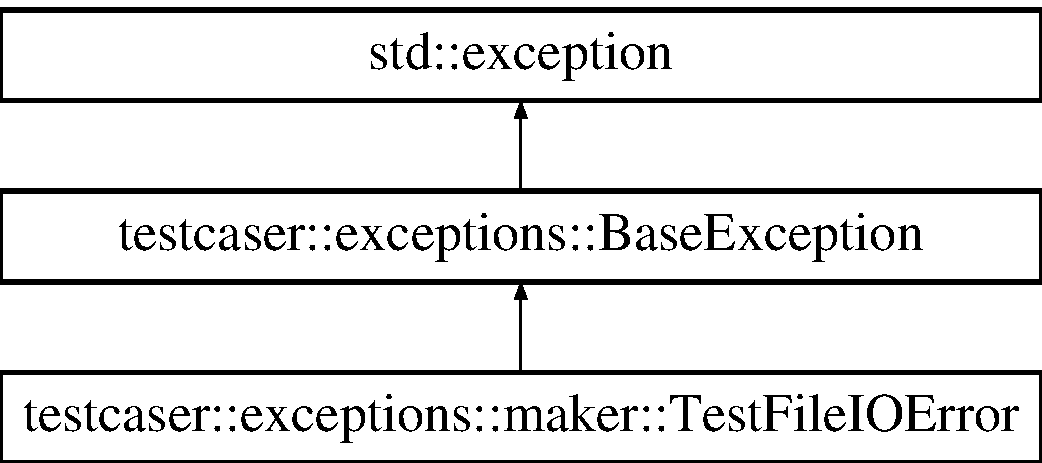
\includegraphics[height=3.000000cm]{classtestcaser_1_1exceptions_1_1maker_1_1TestFileIOError}
\end{center}
\end{figure}
\subsection*{Public Member Functions}
\begin{DoxyCompactItemize}
\item 
\hyperlink{classtestcaser_1_1exceptions_1_1maker_1_1TestFileIOError_a2168ea54454727b86b6e00e5cd8103e0}{Test\+File\+I\+O\+Error} (std\+::string details)
\begin{DoxyCompactList}\small\item\em Construct a new Test File I O Error object. \end{DoxyCompactList}\item 
\mbox{\Hypertarget{classtestcaser_1_1exceptions_1_1maker_1_1TestFileIOError_ab83e748d26f860c9b045535447a383c5}\label{classtestcaser_1_1exceptions_1_1maker_1_1TestFileIOError_ab83e748d26f860c9b045535447a383c5}} 
void \hyperlink{classtestcaser_1_1exceptions_1_1maker_1_1TestFileIOError_ab83e748d26f860c9b045535447a383c5}{add\+\_\+more\+\_\+info} () final override
\begin{DoxyCompactList}\small\item\em adds more information to exception such as what was expected and what was provided. \end{DoxyCompactList}\end{DoxyCompactItemize}
\subsection*{Additional Inherited Members}


\subsection{Detailed Description}
\hyperlink{classtestcaser_1_1exceptions_1_1maker_1_1TestFileIOError}{Test\+File\+I\+O\+Error} exception is thrown as soon as new test-\/case file failed to open or was opened in s state that does not offers write the file. 

\subsection{Constructor \& Destructor Documentation}
\mbox{\Hypertarget{classtestcaser_1_1exceptions_1_1maker_1_1TestFileIOError_a2168ea54454727b86b6e00e5cd8103e0}\label{classtestcaser_1_1exceptions_1_1maker_1_1TestFileIOError_a2168ea54454727b86b6e00e5cd8103e0}} 
\index{testcaser\+::exceptions\+::maker\+::\+Test\+File\+I\+O\+Error@{testcaser\+::exceptions\+::maker\+::\+Test\+File\+I\+O\+Error}!Test\+File\+I\+O\+Error@{Test\+File\+I\+O\+Error}}
\index{Test\+File\+I\+O\+Error@{Test\+File\+I\+O\+Error}!testcaser\+::exceptions\+::maker\+::\+Test\+File\+I\+O\+Error@{testcaser\+::exceptions\+::maker\+::\+Test\+File\+I\+O\+Error}}
\subsubsection{\texorpdfstring{Test\+File\+I\+O\+Error()}{TestFileIOError()}}
{\footnotesize\ttfamily testcaser\+::exceptions\+::maker\+::\+Test\+File\+I\+O\+Error\+::\+Test\+File\+I\+O\+Error (\begin{DoxyParamCaption}\item[{std\+::string}]{details }\end{DoxyParamCaption})\hspace{0.3cm}{\ttfamily [inline]}}



Construct a new Test File I O Error object. 


\begin{DoxyParams}{Parameters}
{\em details} & A Generic message for exception \\
\hline
\end{DoxyParams}


The documentation for this class was generated from the following file\+:\begin{DoxyCompactItemize}
\item 
testcaser/core/exceptions/Build\+Exception.\+hpp\end{DoxyCompactItemize}

\hypertarget{classtestcaser_1_1integrator_1_1VirtualJudge}{}\section{testcaser\+:\+:integrator\+:\+:Virtual\+Judge Class Reference}
\label{classtestcaser_1_1integrator_1_1VirtualJudge}\index{testcaser::integrator::VirtualJudge@{testcaser::integrator::VirtualJudge}}


The \mbox{\hyperlink{classtestcaser_1_1integrator_1_1VirtualJudge}{Virtual\+Judge}} Class use to create a new virtual judge session to run a program.  




{\ttfamily \#include $<$integrator.\+hpp$>$}

\subsection*{Public Member Functions}
\begin{DoxyCompactItemize}
\item 
\mbox{\hyperlink{classtestcaser_1_1integrator_1_1VirtualJudge_a10b68744cc523bcc8abe1ddca7a281dc}{Virtual\+Judge}} ()
\begin{DoxyCompactList}\small\item\em Construct a new \mbox{\hyperlink{classtestcaser_1_1integrator_1_1VirtualJudge}{Virtual\+Judge}} object. Default time limit is 1 sec, 30s is auto exit time when auto exit is false. If program does not exists in 30s although it has passed its time limit, It will recieve a S\+I\+G\+K\+I\+LL. It also defaults 256 MB of memory limit. If not explicitly set by the programmer. \end{DoxyCompactList}\item 
\mbox{\hyperlink{classtestcaser_1_1integrator_1_1VirtualJudge}{Virtual\+Judge}} \mbox{\hyperlink{classtestcaser_1_1integrator_1_1VirtualJudge_a8ac8e323d9f69fb4e1f6ee2e9aa1ae9f}{set\+\_\+memory\+\_\+limit}} (size\+\_\+t kilobyte)
\begin{DoxyCompactList}\small\item\em Set the memory limit to the program to execute. \end{DoxyCompactList}\item 
\mbox{\hyperlink{classtestcaser_1_1integrator_1_1VirtualJudge}{Virtual\+Judge}} \mbox{\hyperlink{classtestcaser_1_1integrator_1_1VirtualJudge_a121272932bb115881ad90be79ad7d0a7}{set\+\_\+time\+\_\+limit}} (size\+\_\+t ssec)
\begin{DoxyCompactList}\small\item\em Set the time limit to the program to execute. \end{DoxyCompactList}\item 
\mbox{\hyperlink{classtestcaser_1_1integrator_1_1VirtualJudge}{Virtual\+Judge}} \mbox{\hyperlink{classtestcaser_1_1integrator_1_1VirtualJudge_ac739270769d85fd09ae35aa53726f8f4}{set\+\_\+auto\+\_\+exit\+\_\+time\+\_\+limit}} (size\+\_\+t ssec)
\begin{DoxyCompactList}\small\item\em Set the auto exit time limit to the program to execute. \end{DoxyCompactList}\item 
\mbox{\hyperlink{classtestcaser_1_1integrator_1_1VirtualJudge}{Virtual\+Judge}} \mbox{\hyperlink{classtestcaser_1_1integrator_1_1VirtualJudge_ad982d30de1a2f9033cb042313d748292}{set\+\_\+input\+\_\+file}} (std\+::string path)
\begin{DoxyCompactList}\small\item\em Set the input source to provide to the program. \end{DoxyCompactList}\item 
\mbox{\hyperlink{classtestcaser_1_1integrator_1_1VirtualJudge}{Virtual\+Judge}} \mbox{\hyperlink{classtestcaser_1_1integrator_1_1VirtualJudge_a9f054aac69019e5f6bde646ccc72effb}{set\+\_\+output\+\_\+file}} (std\+::string path)
\begin{DoxyCompactList}\small\item\em Set the output from a program to write to the given path. \end{DoxyCompactList}\item 
\mbox{\hyperlink{classtestcaser_1_1integrator_1_1VirtualJudge}{Virtual\+Judge}} \mbox{\hyperlink{classtestcaser_1_1integrator_1_1VirtualJudge_ae9fc3d7bf1bf75fc1ec695fe831d16b6}{set\+\_\+binary}} (std\+::string path)
\begin{DoxyCompactList}\small\item\em Set the binary to run the program. This binary will run. \end{DoxyCompactList}\item 
\mbox{\hyperlink{classtestcaser_1_1integrator_1_1VirtualJudge}{Virtual\+Judge}} \mbox{\hyperlink{classtestcaser_1_1integrator_1_1VirtualJudge_a9160dd070c63084495fe6d29cab58cb4}{set\+\_\+auto\+\_\+exit}} (bool terminate=true)
\begin{DoxyCompactList}\small\item\em Set the auto terminate when time or memory limit exceeds. \end{DoxyCompactList}\item 
\mbox{\hyperlink{classtestcaser_1_1integrator_1_1Result}{Result}} \mbox{\hyperlink{classtestcaser_1_1integrator_1_1VirtualJudge_ab50e9c4506fba192fd44fce0f2a21744}{execute}} ()
\begin{DoxyCompactList}\small\item\em Starts the execution of the program after validating if eveyrthing is correct. \end{DoxyCompactList}\end{DoxyCompactItemize}


\subsection{Detailed Description}
The \mbox{\hyperlink{classtestcaser_1_1integrator_1_1VirtualJudge}{Virtual\+Judge}} Class use to create a new virtual judge session to run a program. 



\subsection{Constructor \& Destructor Documentation}
\mbox{\Hypertarget{classtestcaser_1_1integrator_1_1VirtualJudge_a10b68744cc523bcc8abe1ddca7a281dc}\label{classtestcaser_1_1integrator_1_1VirtualJudge_a10b68744cc523bcc8abe1ddca7a281dc}} 
\index{testcaser::integrator::VirtualJudge@{testcaser::integrator::VirtualJudge}!VirtualJudge@{VirtualJudge}}
\index{VirtualJudge@{VirtualJudge}!testcaser::integrator::VirtualJudge@{testcaser::integrator::VirtualJudge}}
\subsubsection{\texorpdfstring{VirtualJudge()}{VirtualJudge()}}
{\footnotesize\ttfamily testcaser\+::integrator\+::\+Virtual\+Judge\+::\+Virtual\+Judge (\begin{DoxyParamCaption}{ }\end{DoxyParamCaption})\hspace{0.3cm}{\ttfamily [inline]}}



Construct a new \mbox{\hyperlink{classtestcaser_1_1integrator_1_1VirtualJudge}{Virtual\+Judge}} object. Default time limit is 1 sec, 30s is auto exit time when auto exit is false. If program does not exists in 30s although it has passed its time limit, It will recieve a S\+I\+G\+K\+I\+LL. It also defaults 256 MB of memory limit. If not explicitly set by the programmer. 



\subsection{Member Function Documentation}
\mbox{\Hypertarget{classtestcaser_1_1integrator_1_1VirtualJudge_ab50e9c4506fba192fd44fce0f2a21744}\label{classtestcaser_1_1integrator_1_1VirtualJudge_ab50e9c4506fba192fd44fce0f2a21744}} 
\index{testcaser::integrator::VirtualJudge@{testcaser::integrator::VirtualJudge}!execute@{execute}}
\index{execute@{execute}!testcaser::integrator::VirtualJudge@{testcaser::integrator::VirtualJudge}}
\subsubsection{\texorpdfstring{execute()}{execute()}}
{\footnotesize\ttfamily \mbox{\hyperlink{classtestcaser_1_1integrator_1_1Result}{Result}} testcaser\+::integrator\+::\+Virtual\+Judge\+::execute (\begin{DoxyParamCaption}{ }\end{DoxyParamCaption})\hspace{0.3cm}{\ttfamily [inline]}}



Starts the execution of the program after validating if eveyrthing is correct. 

\begin{DoxyReturn}{Returns}
\mbox{\hyperlink{classtestcaser_1_1integrator_1_1Result}{Result}} the object that holds the result of the execution of the binary provided. 
\end{DoxyReturn}
\mbox{\Hypertarget{classtestcaser_1_1integrator_1_1VirtualJudge_a9160dd070c63084495fe6d29cab58cb4}\label{classtestcaser_1_1integrator_1_1VirtualJudge_a9160dd070c63084495fe6d29cab58cb4}} 
\index{testcaser::integrator::VirtualJudge@{testcaser::integrator::VirtualJudge}!set\_auto\_exit@{set\_auto\_exit}}
\index{set\_auto\_exit@{set\_auto\_exit}!testcaser::integrator::VirtualJudge@{testcaser::integrator::VirtualJudge}}
\subsubsection{\texorpdfstring{set\_auto\_exit()}{set\_auto\_exit()}}
{\footnotesize\ttfamily \mbox{\hyperlink{classtestcaser_1_1integrator_1_1VirtualJudge}{Virtual\+Judge}} testcaser\+::integrator\+::\+Virtual\+Judge\+::set\+\_\+auto\+\_\+exit (\begin{DoxyParamCaption}\item[{bool}]{terminate = {\ttfamily true} }\end{DoxyParamCaption})\hspace{0.3cm}{\ttfamily [inline]}}



Set the auto terminate when time or memory limit exceeds. 


\begin{DoxyParams}{Parameters}
{\em terminate} & should we terminate the program as soon as time or memory limit allocated is exceeded. \\
\hline
\end{DoxyParams}
\begin{DoxyReturn}{Returns}
\mbox{\hyperlink{classtestcaser_1_1integrator_1_1VirtualJudge}{Virtual\+Judge}} the current (this) object for builder syntax of construction. 
\end{DoxyReturn}
\mbox{\Hypertarget{classtestcaser_1_1integrator_1_1VirtualJudge_ac739270769d85fd09ae35aa53726f8f4}\label{classtestcaser_1_1integrator_1_1VirtualJudge_ac739270769d85fd09ae35aa53726f8f4}} 
\index{testcaser::integrator::VirtualJudge@{testcaser::integrator::VirtualJudge}!set\_auto\_exit\_time\_limit@{set\_auto\_exit\_time\_limit}}
\index{set\_auto\_exit\_time\_limit@{set\_auto\_exit\_time\_limit}!testcaser::integrator::VirtualJudge@{testcaser::integrator::VirtualJudge}}
\subsubsection{\texorpdfstring{set\_auto\_exit\_time\_limit()}{set\_auto\_exit\_time\_limit()}}
{\footnotesize\ttfamily \mbox{\hyperlink{classtestcaser_1_1integrator_1_1VirtualJudge}{Virtual\+Judge}} testcaser\+::integrator\+::\+Virtual\+Judge\+::set\+\_\+auto\+\_\+exit\+\_\+time\+\_\+limit (\begin{DoxyParamCaption}\item[{size\+\_\+t}]{ssec }\end{DoxyParamCaption})\hspace{0.3cm}{\ttfamily [inline]}}



Set the auto exit time limit to the program to execute. 


\begin{DoxyParams}{Parameters}
{\em ssec} & the allocated time in second for program to execute even after it passed the time limit and auto exit is false. It must be atleast 1 second. After this time S\+I\+G\+K\+I\+LL is bound to kill the child. It must be more than time limit. \\
\hline
\end{DoxyParams}
\begin{DoxyReturn}{Returns}
\mbox{\hyperlink{classtestcaser_1_1integrator_1_1VirtualJudge}{Virtual\+Judge}} the current (this) object for builder syntax of construction. 
\end{DoxyReturn}
\mbox{\Hypertarget{classtestcaser_1_1integrator_1_1VirtualJudge_ae9fc3d7bf1bf75fc1ec695fe831d16b6}\label{classtestcaser_1_1integrator_1_1VirtualJudge_ae9fc3d7bf1bf75fc1ec695fe831d16b6}} 
\index{testcaser::integrator::VirtualJudge@{testcaser::integrator::VirtualJudge}!set\_binary@{set\_binary}}
\index{set\_binary@{set\_binary}!testcaser::integrator::VirtualJudge@{testcaser::integrator::VirtualJudge}}
\subsubsection{\texorpdfstring{set\_binary()}{set\_binary()}}
{\footnotesize\ttfamily \mbox{\hyperlink{classtestcaser_1_1integrator_1_1VirtualJudge}{Virtual\+Judge}} testcaser\+::integrator\+::\+Virtual\+Judge\+::set\+\_\+binary (\begin{DoxyParamCaption}\item[{std\+::string}]{path }\end{DoxyParamCaption})\hspace{0.3cm}{\ttfamily [inline]}}



Set the binary to run the program. This binary will run. 


\begin{DoxyParams}{Parameters}
{\em path} & the path to the binary to run and bechmark. \\
\hline
\end{DoxyParams}
\begin{DoxyReturn}{Returns}
\mbox{\hyperlink{classtestcaser_1_1integrator_1_1VirtualJudge}{Virtual\+Judge}} the current (this) object for builder syntax of construction. 
\end{DoxyReturn}
\mbox{\Hypertarget{classtestcaser_1_1integrator_1_1VirtualJudge_ad982d30de1a2f9033cb042313d748292}\label{classtestcaser_1_1integrator_1_1VirtualJudge_ad982d30de1a2f9033cb042313d748292}} 
\index{testcaser::integrator::VirtualJudge@{testcaser::integrator::VirtualJudge}!set\_input\_file@{set\_input\_file}}
\index{set\_input\_file@{set\_input\_file}!testcaser::integrator::VirtualJudge@{testcaser::integrator::VirtualJudge}}
\subsubsection{\texorpdfstring{set\_input\_file()}{set\_input\_file()}}
{\footnotesize\ttfamily \mbox{\hyperlink{classtestcaser_1_1integrator_1_1VirtualJudge}{Virtual\+Judge}} testcaser\+::integrator\+::\+Virtual\+Judge\+::set\+\_\+input\+\_\+file (\begin{DoxyParamCaption}\item[{std\+::string}]{path }\end{DoxyParamCaption})\hspace{0.3cm}{\ttfamily [inline]}}



Set the input source to provide to the program. 


\begin{DoxyParams}{Parameters}
{\em path} & the path of the input file to input to the program. This will be generated by the \mbox{\hyperlink{classtestcaser_1_1maker_1_1TestCaseBuilder}{testcaser\+::maker\+::\+Test\+Case\+Builder}} \\
\hline
\end{DoxyParams}
\begin{DoxyReturn}{Returns}
\mbox{\hyperlink{classtestcaser_1_1integrator_1_1VirtualJudge}{Virtual\+Judge}} the current (this) object for builder syntax of construction. 
\end{DoxyReturn}
\mbox{\Hypertarget{classtestcaser_1_1integrator_1_1VirtualJudge_a8ac8e323d9f69fb4e1f6ee2e9aa1ae9f}\label{classtestcaser_1_1integrator_1_1VirtualJudge_a8ac8e323d9f69fb4e1f6ee2e9aa1ae9f}} 
\index{testcaser::integrator::VirtualJudge@{testcaser::integrator::VirtualJudge}!set\_memory\_limit@{set\_memory\_limit}}
\index{set\_memory\_limit@{set\_memory\_limit}!testcaser::integrator::VirtualJudge@{testcaser::integrator::VirtualJudge}}
\subsubsection{\texorpdfstring{set\_memory\_limit()}{set\_memory\_limit()}}
{\footnotesize\ttfamily \mbox{\hyperlink{classtestcaser_1_1integrator_1_1VirtualJudge}{Virtual\+Judge}} testcaser\+::integrator\+::\+Virtual\+Judge\+::set\+\_\+memory\+\_\+limit (\begin{DoxyParamCaption}\item[{size\+\_\+t}]{kilobyte }\end{DoxyParamCaption})\hspace{0.3cm}{\ttfamily [inline]}}



Set the memory limit to the program to execute. 


\begin{DoxyParams}{Parameters}
{\em kilobyte} & the allocated memory in Kilo\+Bytes. It must be an non-\/negative integer. \\
\hline
\end{DoxyParams}
\begin{DoxyReturn}{Returns}
virtual\+Judge the current (this) object for builder syntax of construction. 
\end{DoxyReturn}
\mbox{\Hypertarget{classtestcaser_1_1integrator_1_1VirtualJudge_a9f054aac69019e5f6bde646ccc72effb}\label{classtestcaser_1_1integrator_1_1VirtualJudge_a9f054aac69019e5f6bde646ccc72effb}} 
\index{testcaser::integrator::VirtualJudge@{testcaser::integrator::VirtualJudge}!set\_output\_file@{set\_output\_file}}
\index{set\_output\_file@{set\_output\_file}!testcaser::integrator::VirtualJudge@{testcaser::integrator::VirtualJudge}}
\subsubsection{\texorpdfstring{set\_output\_file()}{set\_output\_file()}}
{\footnotesize\ttfamily \mbox{\hyperlink{classtestcaser_1_1integrator_1_1VirtualJudge}{Virtual\+Judge}} testcaser\+::integrator\+::\+Virtual\+Judge\+::set\+\_\+output\+\_\+file (\begin{DoxyParamCaption}\item[{std\+::string}]{path }\end{DoxyParamCaption})\hspace{0.3cm}{\ttfamily [inline]}}



Set the output from a program to write to the given path. 


\begin{DoxyParams}{Parameters}
{\em path} & the path to write the output. \\
\hline
\end{DoxyParams}
\begin{DoxyReturn}{Returns}
\mbox{\hyperlink{classtestcaser_1_1integrator_1_1VirtualJudge}{Virtual\+Judge}} the current (this) object for builder syntax of construction. 
\end{DoxyReturn}
\mbox{\Hypertarget{classtestcaser_1_1integrator_1_1VirtualJudge_a121272932bb115881ad90be79ad7d0a7}\label{classtestcaser_1_1integrator_1_1VirtualJudge_a121272932bb115881ad90be79ad7d0a7}} 
\index{testcaser::integrator::VirtualJudge@{testcaser::integrator::VirtualJudge}!set\_time\_limit@{set\_time\_limit}}
\index{set\_time\_limit@{set\_time\_limit}!testcaser::integrator::VirtualJudge@{testcaser::integrator::VirtualJudge}}
\subsubsection{\texorpdfstring{set\_time\_limit()}{set\_time\_limit()}}
{\footnotesize\ttfamily \mbox{\hyperlink{classtestcaser_1_1integrator_1_1VirtualJudge}{Virtual\+Judge}} testcaser\+::integrator\+::\+Virtual\+Judge\+::set\+\_\+time\+\_\+limit (\begin{DoxyParamCaption}\item[{size\+\_\+t}]{ssec }\end{DoxyParamCaption})\hspace{0.3cm}{\ttfamily [inline]}}



Set the time limit to the program to execute. 


\begin{DoxyParams}{Parameters}
{\em ssec} & the allocated time in second for program to execute. It must be atleast 1 second \\
\hline
\end{DoxyParams}
\begin{DoxyReturn}{Returns}
\mbox{\hyperlink{classtestcaser_1_1integrator_1_1VirtualJudge}{Virtual\+Judge}} the current (this) object for builder syntax of construction. 
\end{DoxyReturn}


The documentation for this class was generated from the following file\+:\begin{DoxyCompactItemize}
\item 
testcaser/core/integrator/integrator.\+hpp\end{DoxyCompactItemize}

%--- End generated contents ---

% Index
\backmatter
\newpage
\phantomsection
\clearemptydoublepage
\addcontentsline{toc}{chapter}{Index}
\printindex

\end{document}
